\documentclass{sig-alternate}
\pdfpagewidth=8.5in
\pdfpageheight=11in
\usepackage{float}
%\usepackage{subfigure}
\usepackage{alltt}
\usepackage{color}
\usepackage{graphicx}
 \usepackage{multirow}
\usepackage{epstopdf}
\usepackage{hyperref}
%\usepackage{algorithm2e}
\usepackage{url}
\usepackage{graphicx}
\usepackage{epstopdf}
\usepackage{balance}
\usepackage{tabularx}
\usepackage{array}



\newcommand{\dl}[1]{\textcolor{red}{{\it [DL says: #1]}}}
\usepackage{amssymb,amsmath}
\usepackage{proof,latexsym}
\usepackage{color}
\usepackage{enumerate}

\usepackage{ifthen}
\usepackage{amssymb}

\usepackage{float}
%\usepackage{subfigure}
\usepackage{alltt}
\usepackage{color}
\usepackage{graphicx}
 \usepackage{multirow}
\usepackage{epstopdf}
\usepackage{hyperref}
%\usepackage{algorithm2e}
\usepackage{url}
\usepackage{algorithm}
\usepackage{algorithmicx}
%\usepackage{algorithmic}
\usepackage{epstopdf}
\usepackage{balance}
\usepackage{multirow}
\usepackage{algpseudocode}
%\usepackage{arydshln}

\newcommand{\CodeIn}[1]{{\small\texttt{#1}}}
\newcommand{\CodeOutSize}{\scriptsize}
\newenvironment{CodeOut}{\begin{scriptsize}}{\end{scriptsize}}
\newtheorem{defn}{Definition}
\newtheorem{prop}{Property}

\begin{document}
\newcommand{\nop}[1]{}
\def\concat{\mathit{+\!\!+}}
\def\ln{\hspace{0.12cm}}
\newcommand{\hide}[1]{\hspace*{-5pt}~}


\floatstyle{ruled}
\newfloat{algorithm}{thp}{loa}
\floatname{algorithm}{Algorithm}
\newfloat{procedure}{thp}{loa}
\floatname{procedure}{Procedure}

\newcommand{\ie}{{\sl i.e.}}
\newcommand{\eg}{{\sl e.g.}}
\newcommand{\etc}{{\sl etc.}}

\title{ Information Retrieval and Spectrum Based\\ Bug Localization: Better Together}

% ABSo
% ALoS

%Instance-Specific Fault Localization Approach Leveraging Bug Reports and Program Spectra}

%Adaptive
%Instance-specific
%Localization
%Buggy Methods
%Execution Traces
%Bug Reports
%Suspicious Words




\numberofauthors{1}
\author{\alignauthor Tien-Duy B. Le, Richard J. Oentaryo, and David Lo\\
\affaddr{School of Information Systems} \\
\affaddr{Singapore Management University}\\
\email{\{btdle.2012,roentaryo,davidlo\}@smu.edu.sg}
}

\conferenceinfo{} {}
\CopyrightYear{}
\crdata{}
\clubpenalty=10000
\widowpenalty = 10000

\maketitle
\sloppy
\begin{abstract}
Developers often spend much effort and resources to debug a program. To help the developers debug, numerous information retrieval (IR)-based and spectrum-based bug localization techniques have been devised. IR-based techniques process textual information in bug reports, while spectrum-based techniques process program spectra (i.e., a record of which program elements are executed for each test case). While both techniques ultimately generate a ranked list of program elements that likely contain a bug, they only consider one source of information---either bug reports or program spectra---which is not optimal. In light of this deficiency, this paper presents a new approach dubbed \underline{Net}work-clustered \underline{M}ulti-modal Bug \underline{L}ocalization (NetML), which utilizes multi-modal information from both bug reports and program spectra to localize bugs. NetML facilitates an effective bug localization by carrying out a joint optimization of bug localization error and clustering of both bug reports and program elements (i.e., methods). The clustering is achieved through the incorporation of \emph{network Lasso} regularization, which incentivizes the latent parameters of similar bug reports and similar program elements to be close together.  To estimate the latent parameters of both bug reports and methods, NetML features an adaptive learning procedure based on Newton method that updates the parameters on a per-feature basis. Extensive experiments on 157 real bugs from four software systems have been conducted to evaluate NetML against various state-of-the-art localization methods. The results show that NetML surpasses the best-performing baseline by 48.39\%, 15.49\%, 8.7\%, and 13.92\%, in terms of the number of bugs successfully localized when a developer inspects the top 1, 5, and 10 methods and Mean Average Precision (MAP), respectively.

%In addition to using bug report text and program spectra features (which are akin to the IR-based and spectra-based techniques respectively), NetML also incorporates a hybrid \emph{method suspiciousness} feature that stems from processing both bug report and program spectra information.

%N-AML \textit{adaptively} creates a bug-specific model to map a particular bug to its possible location, and introduces a {\em suspicious words} that are highly associated to a bug. N-AML is an extension of \underline{A}daptive \underline{M}ulti-Modal bug \underline{L}ocalization (AML) which was presented in Foundations of Software Engineering Conference. More specifically, N-AML involves two extensions compared to AML: redefine the function of suspiciousness score between bugs and program elements, and make use of Network Lasso regularization to exploit the similarities amongst different bugs and program elements to localize the bug among list of program elements.  

%We evaluate AML* on 157 real bugs from four software systems, and compare it with AML and state-of-the-art bug localization approaches.
%Experiments show that AML* outperforms the best baselines by at least 119.05\%, 51.85\%, 38.89\%, and 46.74\% in terms of number of bugs successfully localized when a developer inspects 1, 5, and 10 program elements (i.e., top 1, top 5, and top 10), and Mean Average Precision (MAP) respectively. Moreover, the results also show that AML* also outperforms AML by 48.39\%, 15.49\%, 8.7\%, and 13.92\% when the developer investigates top 1, top 5, top 10 methods and MAP respectively. 

%We evaluate N-AML on 157 real bugs from four software systems, and compare it with original multi-modal techniques (i.e. AML). Experiments show that N-AML outperforms AML by at least 48.39\%, 15.49\%, 8.7\%, and 13.92\% in terms of number of bugs successfully localized when a developer inspects 1, 5, and 10 program elements (i.e., top 1, top 5, and top 10), and Mean Average Precision (MAP) respectively. Moreover, we also compare N-AML with the state-of-the-art bug localization approaches. The results demonstrate that N-AML surpasses the best baseline (i.e. PROMESIR) by  119.05\%, 51.85\%, 38.89\%, and 46.74\% in top 1, top 5, top 10 programs, and MAP respectively.

%successfully localize 92 out of the 157 bug reports, which is 27.78\% more than the best baseline, when developers only inspect the top-10 recommended program elements. In terms of Mean Average Precision (MAP), our approach outperforms the best baseline by 28.80\%.

%considering only bugs that can be localized by analyzing the first 10 recommended program elements in a ranked list, our approach successfully localizes faulty methods  in 92 out of 157 bug reports.our approach can achieve a mean average precision (MAP) score of {\color{red}{0.237}} which is substantially higher than the results of the baseline approaches.

%our proposed approach can achieve a success-rate@1 of {\color{red}17.83\%} which is {\color{red}33.33\%} higher than the best baseline.

%These techniques can be grouped to two main families: those that use information retrieval and processes textual description in bug reports to find buggy program elements that are textually similar to the bug reports, and those that analyze failing and correct test case executions and compute suspiciousness scores of program elements that are executed more in the failing rather than successful executions.


\end{abstract}

%\category{H.2.8}{Database Management}{Database Applications}[Data Mining]
%\category{J.4}{Computer Applications}{Social and Behavioral Sciences}[Sociology]

%\terms{Algorithms, Experimentation}
%\keywords{Direct antagonistic community, Mining maximal bi-cliques, Signed social network}


\section{Introduction}\label{sec.intro}
\section{Introduction}
\label{sec.intro}

Debugging bug reports, which often come in a high volume~\cite{AnvikHM05}, has proved to be a difficult task that consumes much resources and time~\cite{tassey02economic}. Various techniques have thus been devised to help developers locate buggy program elements from their symptoms. These symptoms could be in the form of a descriptions of a bug experienced by a user, or a failing test case. These techniques, often collectively referred to as bug (or fault) localization, would analyze the symptoms of a bug and produce a list of program elements ranked based on their likelihood to contain the bug.

Existing bug localization techniques broadly fall into two major categories: \emph{information retrieval} (IR)-based techniques~\cite{Rao:2011:RSL:1985441.1985451,Sisman:2012:IVH:2664446.2664454,Zhou:2012:BFM:2337223.2337226,SahaLKP13}, and \emph{spectrum}-based bug localization techniques~\cite{JH05,Abreu:2009,RR03,ZH02,Zeller2002a,CZ05,LAZJ03,Libl+05,LYFHM05}. The IR-based bug localization techniques typically analyze textual descriptions contained in bug reports and identifier names and comments in source code files. They then return a ranked list of program elements (typically program files) that are the most similar to the bug textual description. The spectrum-based bug localization techniques typically analyze program spectra that corresponds to program elements that are executed by failing and successful execution traces. Likewise, they return a ranked list of program elements (typically program blocks or statements) that are executed more often in the failing rather than correct traces.

% What are the latest trend
% Why multi-modal bug localization make sense?

The above-mentioned approaches, however, only consider one kind of symptom or one source of information, i.e., only bug reports or only execution traces. This is a limiting factor since hints of the location of a bug may be spread in both bug report and execution traces; and some hints may only appear in one but not the other. In this work, we put forward a bug localization approach that addresses the deficiency of existing methods by jointly utilizing both bug reports and execution traces. We refer to this approach as {\em multi-modal bug localization}, as we need to consider multiple modes of inputs (i.e., bug reports and program spectra). Such an approach fits well to developers' debugging activities as illustrated by the following scenarios:

\begin{enumerate}
	\item Developer $D$ is working on a bug report that is submitted to Bugzilla. One of the first tasks that he needs to do is to replicate the bug based on the description in the report. If the bug can be successfully replicated, he will proceed to the debugging step; otherwise, he will mark the bug report as ``WORKSFORME'' and will not continue further~\cite{worksforme}. After $D$ replicates the bug, he has one or a few failing execution traces. He also has a set of regression tests that he can run to get successful execution traces. Thus, after the replication process, $D$ has {\em both} the textual description of the bug and a program spectra that characterizes the bug. With this, $D$ can proceed to use multi-modal bug localization.
	\item  Developer $D$ runs a regression test suite and some test cases fail. Based on his experience, $D$ has some idea why the test cases fail. $D$ can create a textual document describing the bug. At the end of this step, $D$ has {\em both} program spectra and textual bug description, and can proceed to use multi-modal bug localization which will leverage not only the program spectra but also $D$'s domain knowledge to locate the bug.
\end{enumerate}

% Although no multi-modal bug localization technique has been proposed in the literature, there are a few multi-modal feature location techniques. These techniques process both feature description and program spectra to recommend program elements (typically program methods) that implement a corresponding feature~\cite{PoshyvanykGMAR07,LiuMPR07,DitRP13}. These feature location approaches can be adapted to locate buggy program elements by replacing feature descriptions with bug reports and feature spectra with buggy program spectra. Unfortunately, our experiment (see Section~\ref{sec.exp}) shows that the performance of such adapted approaches are not optimal yet.

\begin{figure*}[!t]
	\centering
	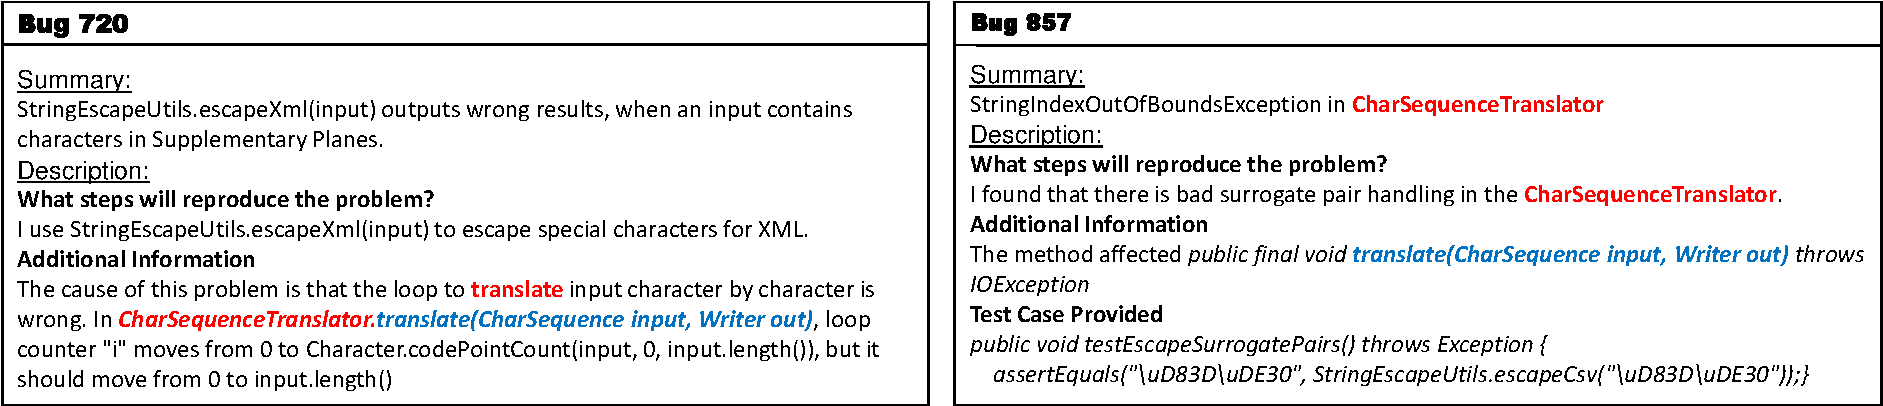
\includegraphics[width=\textwidth]{bug_example.pdf}
	\caption{Example of two bug reports which have same faulty method in project Lang}
	\label{fig:bug_motivation}
\end{figure*}

It is worth noting that our work focuses on localizing a bug to the \emph{method} that contains it. Historically, most IR-based bug localization techniques aim at finding buggy files~\cite{Rao:2011:RSL:1985441.1985451,Sisman:2012:IVH:2664446.2664454,Zhou:2012:BFM:2337223.2337226,SahaLKP13}, while most spectrum-based techniques find buggy lines~\cite{JH05,Abreu:2009,RR03}. Although it is useful to localize a bug to the file that contains it, the file size can be big and developers still need to go through a lot of code to find the few lines that contain the bug. On the other hand, while localizing a bug to the line that contains it is also useful, a bug often spans across multiple lines. Furthermore, developers often do not have ``perfect bug understanding''~\cite{ParninO11} and thus by just looking at a line of code, developers often cannot determine whether it is the location of the bug and/or understand the bug well enough to fix it. Localization at the method level presents a good tradeoff; a method is not as big as a file, but it often contains sufficient context needed to help developers understand a bug.

%Poshyvanyk et al. proposed an approach named PROMESIR that computes weighted sums of scores returned by an IR-based feature location solution and a spectrum-based feature location solution, and ranks program elements based on these scores~\cite{PoshyvanykGMAR07}. Liu et al. proposed an approach named SITIR which filters program elements returned by an IR-based feature location solution if they are not executed in a failing execution trace~\cite{LiuMPR07}. Dit et al. use HITS, a popular algorithm that ranks the importance of nodes in a graph, to filter program elements returned by SITIR~\cite{DitRP13}. Their paper highlights two best performing variants that outperform SITIR, which differ on how the graph to be analyzed by HITS is generated; we refer to these variants as $DIT^{A}$ and $DIT^{B}$ in this paper.

% How our approach might help ? Why the approach would work ? Intuition. Cite Parnin and Orso's work here.
% Our multi-modal bug localization approach improves previous multi-modal approaches based on two intuitions. First, we note that there are a wide variety of bugs~\cite{ThungWLJ12,XiaZLZ13} and different bugs often require different treatments. Thus, there is a need for a bug localization technique that is adaptive to different types of bugs. Past approaches~\cite{LiuMPR07,DitRP13,PoshyvanykGMAR07} propose a one-size-fits-all solution. Here, we propose an instance-specific solution that considers each bug individually and tunes various parameters based on the characteristic of the bug. Second, Parnin and Orso~\cite{ParninO11} highlight in their study that some words are useful in localizing bugs and suggest that ``future research could also investigate ways to automatically suggest or highlight terms that might be related to a failure''. Based on their observation, we design an approach that can automatically highlight {\em suspicious words} and use them to localize bugs.



In this paper, we present a new approach called the \underline{Net}work-clustered \underline{M}ulti-modal Bug \underline{L}ocalization (NetML), which works based on three main intuitions. Firstly, it is established that a wide variety of bugs exist~\cite{ThungWLJ12,XiaZLZ13}, and different bugs often require different treatments. Hence, there is a need to have separate latent parameters for different bugs, which are tailored to the characteristics of the individual bugs. Similarly, different program elements (or methods in this work) are of different nature, and should be characterized using separate latent parameters. Secondly, Parnin and Orso~\cite{ParninO11} found in their studies that some words are more useful in localizing bugs, and suggested that ``future research could also investigate ways to automatically suggest or highlight terms that might be related to a failure''. NetML provides such capability by incorporating \emph{method suspiciousness} feature, which allows us to automatically highlight suspicious terms and use them to localize bugs. Lastly, we recognize that bugs and program elements are \emph{not} completely independent, and some bugs (or methods) may be more similar to certain bugs (or methods) than to others. As such, similar bugs (or methods) should have latent parameters that are close together, which can then be exploited to localize bugs more effectively. 

Figure~\ref{fig:bug_motivation} presents an example of two bug reports which motivate our intuitions. Bug 720 has an ``outputs wrong results'' error when an input contains ``characters in \textit{Supplementary Planes}'' whereas Bug 857 contains ``\textit{StringIndexOutOfBoundsException}'' error. These two bugs ultimately reside in the \texttt{translate} method in the \texttt{CharSequenceTranslator.java} program. Based on text descriptions, these two bugs are quite independently since they provide two different bugs in Lang. However, Bug 720 and Bug 857 should be similar since they share the same \texttt{translate} method and \texttt{CharSequenceTranslator.java} program. At a text level space, we are unable to capture the similarity between two bug reports. 

Some of these intuitions have already been captured in our recent work---dubbed \underline{A}daptive \underline{M}ulti-Modal Bug \underline{L}ocalization (AML)~\cite{Le:2015:IRS:2786805.2786880}--- which we extend in this journal paper. In particular, AML already incorporates the ideas of adaptively computing separate latent parameters for each bug report, and of computing the method suspiciousness score.
%where we proposed \underline{A}daptive \underline{M}ulti-modal bug \underline{L}ocalization (i.e., AML) consisting of three different components:  AML$^\text{Text}$, AML$^\text{Spectra}$, and AML$^\text{SuspWord}$. AML$^\text{Text}$ only considers the textual description in bug reports, and AML$^\text{Spectra}$ only considers program spectra. On the other hand, AML$^\text{SuspWord}$ takes into account suspicious words learned by analyzing textual description and program spectra together. Typically, AML$^\text{SuspWord}$ computes the {\em suspicious scores} of words that appear as comments or identifiers of various program elements. It associates a program element to a set of words and the suspiciousness of a word can then be computed based on the number of times the corresponding program elements appear in failing or correct execution traces. Each of these components would output a score for each program element, and AML computes the weighted sum of these scores by forcing all program elements to share the same tuple of component weights ($\alpha, \beta, \gamma$) which corresponds to AML$^\text{Text}$, AML$^\text{Spectra}$, and AML$^\text{SuspWord}$, respectively. 
%. The final score is {\em adaptively} computed for each individual bug by tuning these weights. 
However, the current AML approach exhibits two main shortcomings. Firstly, AML only has the concept of latent parameters for bug reports, but not for program elements (or methods). As such, it is not able to capture the variation in the (latent) characteristics of different program elements (methods), which may limit its effectiveness in localizing a bug. Secondly, the latent parameters of each bug report are learned independently of those of other bug reports. As a result, AML is unable to take advantage of the clustering/similarity traits of different bug reports in the localization process.

%\begin{itemize}
%	\item First, the final suspiciousness score only assumed that all the program elements share the same parameter vector of bug report. In practice, each program element not only considers the parameter vector of bug reports but also share the parameter of program elements. For example, we call $f_{ij}$ as the suspiciousness score of program element $i$ related to bug $j$, and $sim_{ij}$ measures the similarity between program element $m_i$ and $m_j$. Assuming that our dataset only includes three program elements which are $m_1$, $m_2$, $m_3$ and one bug report $b_1$, and their suspiciousness score results are ranked as $f_{11} > f_{21} > f_{31}$. Moreover, we also assume that 
	%the program element $m_1$ and $m_3$ have a high similarity score compared to $m_2$. In other words, %
	%the similarity scores of $m_1$, $m_2$ and $m_3$ are expressed as following ($sim_{13} \gg sim_{12}$) and ($sim_{13} \gg sim_{23}$). According to the suspiciousness score ranking, $m_1$ has highly related to bug report $b_1$. Furthermore, $m_1$ and $m_2$ have a high similarity score compared to $m_2$, and hence our suspiciousness ranking should be $(f_{11} \approx f_{31}) > f_{21}$. However, AML only assumes that each program element shares the same weight vector of bug report without considering its distinctive functionalities and properties, leading to the suspiciousness ranking score of AML may be inaccurate. 
	%rank of similarity scores between different program elements are presented as ($sim_{13} \gg sim_{12}$)
	%\item Second, the parameter vector of bug report $b$ is learned independently of other bug reports, without exploiting the clustering and/or similarity properties of different bug reports. For example, the suspiciousness scores of program element $m_1$ with three different bug reports $b_1$, $b_2$, and $b_3$ are ranked as $f_{11} > f_{12} > f_{13}$. Assuming that two bug reports $b_1$ and $b_3$ are highly correlated, hence the suspiciousness scores of program element $m_1$ with these two bug reports should be similar (i.e., $f_{11} \approx f_{13}$). In original AML, the parameter vector of each bug report is trained independently without considering its neighbors, hence AML may not accurately reflect the suspiciousness scores between program elements and bug reports. 
%\end{itemize}

The proposed NetML method addresses these shortcomings by performing joint optimization of localization loss function and clustering of both bug reports and methods. Specifically, it generalizes AML in two important ways. Firstly, NetML features two sets of latent parameters---one for bug reports and the other for methods. The incorporation of the (additional) latent method parameters provides NetML with a higher degree of freedom to model the rich variations of different bug reports and methods more accurately. Secondly, NetML augments the network Lasso regularization~\cite{Hallac:2015:NLC:2783258.2783313} in its parameter learning procedure, which enforces similar bug reports (and methods) to have similar latent parameters. It must be noted that, different from the conventional network Lasso that deals with only a single network (graph), we impose regularization over two networks, i.e., bug report similarity and method similarity graphs. This allows us to achieve simultaneous clustering of bug reports and methods, and exploit the similarity traits to achieve a more effective bug localization.

%but also introduces redefine the function of suspiciousness score between bug reports and program elements by taking into account the distinctive functionalities and properties of each program elements. In the second extension, we exploit the similarities amongst different bug reports by taking advantage of the Network Lasso regularization~\cite{Hallac:2015:NLC:2783258.2783313}. Moreover we also consider the relationship between different program elements, hence our approach involves optimizing over two graphs (i.e., bugs and program elements). This is different from traditional Network Lasso that only deals with a single graph.

% The overall architecture of our approach.
% In our previous work, we propose \underline{A}daptive \underline{M}ulti-modal bug \underline{L}ocalization (AML) that realizes the above mentioned intuitions~\cite{Le:2015:IRS:2786805.2786880}. It consists of three components: AML$^\text{Text}$, AML$^\text{Spectra}$, and AML$^\text{SuspWord}$. AML$^\text{Text}$ only considers the textual description in bug reports, and AML$^\text{Spectra}$ only considers program spectra. On the other hand, AML$^\text{SuspWord}$ takes into account suspicious words learned by analyzing textual description and program spectra together. AML$^\text{SuspWord}$ computes the {\em suspicious scores} of words that appear as comments or identifiers of various program elements. It associates a program element to a set of words and the suspiciousness of a word can then be computed based on the number of times the corresponding program elements appear in failing or correct execution traces. Each of these components would output a score for each program element, and AML computes the weighted sum of these scores. The final score is {\em adaptively} computed for each individual bug by tuning these weights.
%Our goal is to infer the best integration of the three components to maximize suspiciousness scores of faulty program elements in resultant ranked lists.



% by leveraging  network lasso~\cite{Hallac:2015:NLC:2783258.2783313} to accurately tune weights of AML$^\text{Text}$, AML$^\text{Spectra}$, and AML$^\text{SuspWord}$. 

%\dl{Is the following statement correct?, Duy: this sounds correct.}


% Each of   AML$^\text{Text}$, AML$^\text{Spectra}$, and AML$^\text{SuspWord}$  component takes as input a method $m$, and outputs a score indicating the likelihood of $m$ to be faulty. 
%The  final suspiciousness score of $m$ is a weighted sum of scores returned by these components.
%AML's adaptive tuning algorithm is limited to compute these weighted sums by forcing all methods to share the same tuple of component weights: $(\alpha,\beta,\gamma)$ which corresponds to AML$^\text{Text}$, AML$^\text{Spectra}$, and AML$^\text{SuspWord}$, respectively.  
%However, two  methods $m_1$ and $m_2$ that have distinctive functionalities and properties should be assigned with two different tuples of $(\alpha,\beta,\gamma)$. Therefore, 
%AML's integrator component limits the diversity in output final scores. That makes it difficult to separate  faulty methods from  the other ones.
%To address the issue ,in this journal paper, we propose  AML* that generalizes AML's tuning algorithms. Intuitively, AML* allows each method has a distinctive tuple of  component weight $(\alpha,\beta,\gamma)$. Furthermore,  AML* takes into account of the relationship between bug reports and program elements to construct a novel tuning algorithm, inspired by Network Lasso~\cite{Hallac:2015:NLC:2783258.2783313}. {\color{red}Duy: please modify paragraph if needed. Need some suggestions from Richard?}



% Experiment results
%We have evaluated our solution using a dataset of 157 real bugs from four medium to large software systems: AspectJ, Ant, Lucene, and Rhino. We collected real bug reports and real test cases from these systems. The test cases are run to generate program spectra. We have compared our approach against 3 state-of-the-art multi-modal feature localization techniques (i.e., PROMESIR~\cite{PoshyvanykGMAR07}, DIT$^{A}$ and DIT$^{B}$~\cite{DitRP13}), a state-of-the-art IR-based bug localization technique~\cite{YeBL14}, and a state-of-the-art spectrum-based bug localization technique~\cite{XuanM14}. We evaluated our approach based on two evaluation metrics: number of bugs localized by inspecting the top N program elements (Top N) and mean average precision (MAP). Top N and MAP are widely used in past bug localization studies, e.g.,~\cite{Rao:2011:RSL:1985441.1985451,Sisman:2012:IVH:2664446.2664454,Zhou:2012:BFM:2337223.2337226,SahaLKP13}. Top N is in line with the observation of Parnin and Orso, who highlight that developers care about absolute rank and they often will stop inspecting program elements, if they do not get promising results when inspecting the top ranked program elements~\cite{ParninO11}. MAP is a standard information retrieval metric to evaluate the effectiveness of a ranking technique~\cite{Manning2008}. Our experiment results highlight that, among the 157 bugs, AML can successfully localize 31, 71, and 92 bugs when developers only inspect the top 1, top 5, and top 10 methods in the lists that AML produces respectively. AML can successfully localize 47.62\%, 31.48\%, and 27.78\% more bugs than the best baseline when developers only inspect the top 1, top 5, and top 10 methods, respectively. In terms of MAP, AML outperforms the best performing baseline by 28.80\%.

To evaluate the efficacy of the NetML approach, we conducted experiments using a dataset of 157 real bugs from four medium to large software systems: AspectJ, Ant, Lucene, and Rhino. All real bug reports and real test cases were collected from these systems. The test cases were run to generate program spectra. We compare NetML with our previous AML method. Additionally, we evaluate our approach against three  state-of-the-art multi-modal feature localization techniques (i.e., PROMESIR~\cite{PoshyvanykGMAR07}, DIT$^{A}$ and DIT$^{B}$~\cite{DitRP13}), a state-of-the-art IR-based bug localization technique~\cite{YeBL14}, and a state-of-the-art spectrum-based bug localization technique~\cite{XuanM14}. We use two well-known evaluation metrics to estimate the performance of our approach: number of bugs localized by inspecting the top N program elements (Top N) and mean average precision (MAP). We note that top N and MAP are widely used in past bug localization studies, e.g.,~\cite{Rao:2011:RSL:1985441.1985451,Sisman:2012:IVH:2664446.2664454,Zhou:2012:BFM:2337223.2337226,SahaLKP13}.
%Top N is in line with the observation of Parnin and Orso, who highlight that developers care about absolute rank and they often will stop inspecting program elements, if they do not get promising results when inspecting the top ranked program elements~\cite{ParninO11}. MAP is a standard information retrieval metric to evaluate the effectiveness of a ranking technique~\cite{Manning2008}. 
Our experiment results demonstrate that, among the 157 bugs, NetML can successfully localize 46, 82, and 100 bugs when developers only inspect the top 1, top 5, and top 10 methods in the lists that NetML produces, respectively. These constitute 48.39\%, 15.49\%, 8.7\%, and 13.92\% improvements over AML (which is the second best method in our benchmark), in terms of Top 1, Top 5 , Top 10, and MAP results respectively.

%AML can successfully localize 47.62\%, 31.48\%, and 27.78\% more bugs than the best baseline when developers only inspect the top 1, top 5, and top 10 methods, respectively. In terms of MAP, AML outperforms the best performing baseline by 28.80\%.
%We have evaluated our solution using a dataset of 157 real bugs from four medium to large software systems: AspectJ, Ant, Lucene, and Rhino. We collected real bug reports and real test cases from these systems. The test cases are run to generate program spectra. We have compared our approach against 3 state-of-the-art multi-modal feature localization techniques (i.e., PROMESIR~\cite{PoshyvanykGMAR07}, DIT$^{A}$ and DIT$^{B}$~\cite{DitRP13}), a state-of-the-art IR-based bug localization technique~\cite{YeBL14}, and a state-of-the-art spectrum-based bug localization technique~\cite{XuanM14}. We evaluated our approach based on two evaluation metrics: number of bugs localized by inspecting the top N program elements (Top N) and mean average precision (MAP). Top N and MAP are widely used in past bug localization studies, e.g.,~\cite{RaoK11,SismanK12,Zhou:2012:BFM:2337223.2337226,SahaLKP13}. Top N is in line with the observation of Parnin and Orso, who highlight that developers care about absolute rank and they often will stop inspecting program elements, if they do not get promising results when inspecting the top ranked program elements~\cite{ParninO11}. MAP is a standard information retrieval metric to evaluate the effectiveness of a ranking technique~\cite{Manning2008}. Our experiment results highlight that, among the 157 bugs, AML can successfully localize 31, 71, and 92 bugs when developers only inspect the top 1, top 5, and top 10 methods in the lists that AML produces respectively. AML can successfully localize 47.62\%, 31.48\%, 27.78\%  more bugs than the best baseline when developers only inspect the top 1, top 5, and top 10 methods, respectively. In terms of MAP, AML outperforms the best performing baseline by 28.80\%.  
%47.62\%, 33.33\%, 27.78\%, and 28.80\%


%Thus, we compute a measure we refer to as success-count@N that measures the number of bugs that can be localized by a bug localization technique when a user only inspects the top $N$ highest ranked program elements. a Top 1, Top 5, and Top 10 scores of 31 MAP score of 0.237, which is significantly higher than the performance of PROMESIR and DIT approaches.

%The MAP score of AML is higher than those of PROMESIR, DIT$^\text{A}$ and DIT$^\text{B}$ by 29.20\%, 100.44\%, and 111.77\% respectively. In terms of success-count@1, success-count@5, and success-count@10, AML can achieve success-counts of 31, 72, and 92 out of 157 bugs, respectively. The success-count@1 of AML is higher than those of PROMESIR, DIT$^\text{A}$ and DIT$^\text{B}$ by 47.62\%, 106.67\%, and 121.43\%, respectively. The success-count@5 of AML is higher than those of PROMESIR, DIT$^\text{A}$ and DIT$^\text{B}$ by 33.33\%, 125.00\%, and 132.26\%, respectively. Similarly,  the success-count@10 of AML is higher than those of PROMESIR, DIT$^\text{A}$ and DIT$^\text{B}$ by 27.78\%, 80.39\%, and 87.76\%, respectively.

% We have also performed a Mann-Whitney U test and find that the difference is significant.
% List of contributions
We summarize the key contributions of this paper below:

\begin{enumerate}
\item We present a novel multi-modal bug localization method that adaptively learns two sets of latent parameters that characterize each bug report and method, respectively. We are also the first to incorporate the network Lasso regularization on both bug report and method similarity networks, which facilitates an effective joint optimization of bug localization quality and clustering of both bug reports and methods.  
\item We develop an adaptive learning procedure based on Newton update to jointly update the latent parameters of bug reports and methods on a per-feature basis. The procedure is based on the formulation of strict convex loss function, which provides a theoretical guarantee that any minimum found will be globally optimal. %Upon request, the codes can be made publicly available later.
\item We have extensively evaluated NetML on a dataset of 157 real bugs from four software systems using real bug reports and test cases. Our statistical significance tests reveal that NetML improves upon state-of-the-art bug localization approaches by a substantial margin.
\end{enumerate}


	
%\item We are the first to build an adaptive algorithm for multi-modal bug localization. Different from past approaches which are one-size-fits-all, our approach is instance-specific and considers each individual bug to tune various parameters or weights of components (i.e., $\text{AML}^\text{Text}$, $\text{AML}^\text{SuspWord}$, and $\text{AML}^\text{Spectra}$).
%\item We are the first to compute suspicious words and use these words to help bug localization. Past studies only compute suspiciousness scores of program elements.
%\item We develop a probabilistic-based iterative optimization procedure to find the best linear combination of AML components (i.e., $\text{AML}^\text{Text}$, $\text{AML}^\text{SuspWord}$, and $\text{AML}^\text{Spectra}$) that maximizes the posterior probability of bug localization. The procedure features an efficient and balanced sampling strategy to gracefully handle the skewed distribution of the faulty vs. non-faulty methods (i.e., given a bug, there are more non-faulty methods than faulty ones in a code base).
%\item We propose a  generalized procedure that further optimizes the combinations of AML components (i.e., $\text{AML}^\text{Text}$, $\text{AML}^\text{SuspWord}$, and $\text{AML}^\text{Spectra}$), and call it as AML*. The procedure assigns a distinctive tuple of weights for every method and  takes into account the relationship of bug reports and program methods. {\color{red} Duy: please modify if needed.}



% Structure of the paper
The remainder of this paper is organized as follows. In Section~\ref{sec.prelim}, we present background information on IR-based and spectrum-based bug localization approaches. Section~\ref{sec.approach} subsequently elaborates the proposed NetML in greater details. In Section~\ref{sec.exp}, we present our dataset, evaluation metrics, and experiment results. Section~\ref{sec.related} then provides an overview of key related works. We finally conclude this paper and discuss future works in Section~\ref{sec.conclusion}.



\section{Background}\label{sec.prelim}
\section{Background}
\label{sec.prelim}

In this section, we present some background material on IR-based and spectrum-based bug localization.

%Section~\ref{sec:irbasedbl} first presents IR-based bug localization. Section~\ref{sec:spectrumbasedbl} next presents spectrum-based bug localization.

%\label{sec:irbasedbl}

\subsection{IR-Based Bug Localization}
\label{sec.IR-based} 

IR-based bug localization techniques consider an input bug report (i.e., the text in the summary and description of the bug report as a query, and program elements in a code base as documents, and employ IR techniques to sort the program elements based on their relevance with the query. The intuition behind these techniques is that program elements sharing many common words with the input bug report are likely to be relevant to the bug. By using text retrieval models, IR-based bug localization computes the similarities between various program elements and the input bug report. Then, program elements are sorted in descending order of their textual similarities to the bug report, and sent to developers for manual inspection.

%\begin{table}[t]
%	\centering
%%	\caption{Bug Report 54460 of Apache Ant}
%    \begin{tabular}{|p{7.5cm}|}
%    \hline
%    \textbf{Bug 54460}
%    
%    \texttt{Summary:} Base64Converter not properly handling bytes with MSB set (not masking byte to int conversion)
%    
%    \texttt{Description:} Base64Converter not properly bytes with MSB set (not masking byte to int conversion).
%    
%    Every 3rd byte taken for conversion (least significant in triplet is not being masked with added to integer, if the msb is set this leads to a signed extension which overwrites the previous two bytes with all ones \dots \\ \hline
%    
%    \end{tabular}
%    \label{fig:bug_example}
%\end{table}

%Figure~\ref{fig:bug_example} shows an example bug report submitted to Bugzilla, which  is obtained from {\url{https://issues.apache.org/bugzilla/show_bug.cgi?id=54460}}  and its summary and description fields. An IR-based bug localization technique then employs an information retrieval technique to recover relevant documents from the query.

%IR-Based bug localization takes as input a textual bug report (the summary and description of a bug) and outputs a ranked list of program elements sorted by the likelihood of them containing the bug. Developers then investigate the program elements in the ranked list, one at a time, to find the faulty program element.
%These two steps are performed as follows:

All IR-based bug localization techniques need to extract textual contents from source code files and preprocess textual contents (either from bug reports or source code files). First, comments and identifier names are extracted from source code files. These can be extracted by employing a simple parser. In this work, we use JDT~\cite{jdt_link} to recover the comments and identifier names from source code. Next, after the textual contents from source code and bug reports are obtained, we need to preprocess them. The purpose of text preprocessing is to standardize words in source code and bug reports. There are three main steps: text normalization, stopword removal, and stemming:

\begin{enumerate}
	\item Text normalization breaks an identifier into its constituent words (tokens), following camel casing convention. Following the work by Saha et al.~\cite{SahaLKP13}, we also keep the original identifier names.
	\item Stopword removal removes punctuation marks, special symbols, number literals, and common stopwords~\cite{stopword_link}. It also removes programming keywords such as $\mathit{if}$, $\mathit{for}$, $\mathit{while}$, etc., which usually appear too frequently to be useful to differentiate between documents.
	\item Stemming simplifies English words into their root forms. For example, ''processed``, ''processing``, and ''processes`` are all simplified to ''process``. This increases the chance of a query and a document to share some common words. We use the popular Porter Stemming algorithm~\cite{P80}.
\end{enumerate}



Numerous IR techniques have been employed for bug localization. We highlight a popular IR technique namely \emph{Vector Space Model} (VSM). In VSM, queries and documents are represented as vectors of weights, where each weight corresponds to a term. The value of each weight is usually the \textit{term frequency\textemdash inverse document frequency} (TF-IDF)~\cite{Ramos1999} of the corresponding word. Term frequency refers to the number of times a word appears in a document. Inverse document frequency refers to the number of documents in a corpus (i.e., a collection of documents) that contain the word. The higher the term frequency and inverse document frequency of a word, the more important the word would be. In this work, given a document $d$ and a corpus $C$, we compute the TF-IDF weight of a word $w$ as follows:
\begin{align}
weight(w,d) &= \text{TF-IDF}(w,d,C) \nonumber\\
            &= \log(f(w,d)+1) \times \log\frac{|C|}{|{d_i\in C : w \in d_i }|} \nonumber
\end{align}
where $f(w,d)$ is the number of times $w$ appears in $d$.
%, and $d_i \in C$ means document $d_i$ is in the set of documents $C$. Similarly, $w \in d_i$ means word $w$ belongs to document $d_i$.

%\begin{figure}[!t]
%\centering
%\fbox{
%\includegraphics[bb=83 532 345 639,width=0.85\linewidth]{example.eps}
%}\vspace{-0.2cm}\caption{Bug Report 54460 of Apache Ant}\vspace{-0.3cm}
%\label{fig:bug_example}
%\end{figure}


%\begin{figure}[!t]
%\centering
%
%    \begin{tabular}{|p{0.95\columnwidth}|}
%    \hline
%    \textbf{Bug 54460}\\ 
%    \\%\texttt{Date:} 22 Jan, 2013\\
%    \texttt{Summary:} 
%    Base64Converter not properly handling bytes with MSB set (not masking byte to int conversion)\\    
%   \\
%    \texttt{Description:}
%    Every 3rd byte taken for conversion (least significant in triplet is not being masked with added to integer, if the msb is set this leads to a signed extension which overwrites the previous two bytes with all ones \dots\\
%    \hline
%    \end{tabular}
%
%\caption{Bug Report 54460 of Apache Ant}
%\label{fig:bug_example}
%\end{figure}


After computing a vector of weights for the query and each document in the corpus, we calculate the cosine similarity of the query and document vectors. The cosine similarity between query $q$ and document $d$ is given by:
\begin{align}
\label{eqn:cosine_sim}
\mathit{sim}(q,d) = \frac{\sum\limits_{w\in (q\bigcap d)} \mathit{weight}(w,q) \times \mathit{weight}(w,d)}{\sqrt{\sum\limits_{w\in q}\mathit{weight}(w,q)^{2}} \times \sqrt{\sum\limits_{w\in d}\mathit{weight}(w,d)^{2}}}
\end{align}
where $w\in (q\bigcap d)$ means word $w$ appears both in the query $q$ and document $d$. Also, $\mathit{weight}(w,q)$ refers to the weight of word $w$ in the query $q$'s vector. Similarly, $\mathit{weight}(w,d)$ refers to the weight of word $w$ in the document $d$'s vector.

%In our paper, we use the following formula to calculate TF-IDF weight of word $w$ in document $d$ given a set of document $C$:
%\begin{equation}
%\textit{TF-IDF}(w,d,C)=\log(f(w,d)+1) \times \log\frac{|C|}{|{d_i\in C : w \in d_i }|}
%\label{eq:tfidf}
%\end{equation}
%
%In comparison with spectrum-based fault localization techniques, IR based bug localization techniques are less costly, as they require no execution traces of the target program on the input set of test cases. In our paper, we propose an approach to integrate spectrum-based fault localization with IR based bug localization to maximize the ranking of faulty code units (i.e., methods).

%\subsection{}\label{sec:spectrumbasedbl}

\subsection{Spectrum-Based Bug Localization} 
\label{sec.spectrum-based}

Spectrum-based bug localization (SBBL)---also known as spectrum-based fault localization (SBFL)---takes as input a faulty program and two sets of test cases. One is a set of failed test cases, and the other one is a set of passed test cases. SBBL then instruments the target program, and records program spectra that are collected when the set of failed and passed test cases are run on the instrumented program. Each of the collected program spectrum contains information of program elements that are executed by a test case. Various tools can be used to collect program spectra as a set of test cases are run. In this work, we use Cobertura~\cite{cobertura_link}.

\begin{table}[!t]
	\caption{Raw Statistics for Program Element $e$}
	\center
    \begin{tabular}{|r|c|c|}
    \hline
    ~                 & e is \textit{executed} & e is \textit{not executed} \\ 
    \hline
    \hline

    {unsuccessful} test & $n_f(e)$             & $n_f(\bar e)$                 \\ 
    %\hline
    {successful} test   & $n_s(e)$             &$n_s(\bar e)$              \\ \hline
    \end{tabular}
    \label{tab:sbfl_matrix}
\end{table}

Based on this spectra, SBBL typically computes some raw statistics for every program element. Tables \ref{tab:sbfl_matrix} and \ref{tab:sbfl_notations} summarize some raw statistics that can be computed for a program element $e$, given a program spectra $p$. These statistics are the counts of unsuccessful (i.e., failed), and successful (i.e., passed) test cases that execute or do not execute $e$. If a successful test case executes program element $e$, then we increase $n_s(e, p)$ by one unit. Similarly, if an unsuccessful test case executes program element $e$, then we increase $n_f(e, p)$ by one unit. SBBL uses these statistics to calculate the suspiciousness scores of each program element. The higher the suspiciousness score, the more likely the corresponding program element is the faulty element. After the suspiciousness scores of all program elements are computed, program elements are then sorted in descending order of their suspiciousness scores, and sent to developers for manual inspection.

%\noindent
%\textbf{Spectrum-Based Bug Localization using Tarantula:} 

Different SBBL techniques have used different formulas to calculate the suspiciousness scores. Among these techniques, Tarantula is a popular one~\cite{JH05}. Using the notation in Table \ref{tab:sbfl_notations}, the following is the formula that Tarantula uses to compute the suspiciousness score of program element $e$, given program spectra $p$:
\begin{align}
\label{eqn:tarantula}
Tarantula(e, p)=\frac{\frac{n_f(e, p)}{n_f(p)}}{\frac{n_f(e, p)}{n_f(p)}+\frac{n_s(e, p)}{n_s(p)}}	
\end{align}
The main idea of Tarantula is that program elements that are executed by failed test cases are more likely to be faulty than those that are not executed. Thus, Tarantula assigns a non-zero score to program element $e$ that has $n_f(e, p) > 0$. 

\begin{table}[tb]
	\centering
	\caption{Raw Statistic Description}
    \begin{tabular}{|p{1.3cm}|p{5.5cm}|}
    \hline
    \textbf{Notation} & \textbf{Description} \\ \hline \hline
  \multirow{2}{*}{$n_f(e, p)$}        & Number of unsuccessful test cases executing program element $e$ in program spectra $p$          \\ \hline
     \multirow{2}{*}{$n_f(\bar{e}, p)$}        & Number of unsuccessful test cases that do not execute program element $e$ in program spectra $p$           \\ \hline
    \multirow{2}{*} {$n_s(e, p)$}         & Number of successful test cases that execute program element $e$ in program spectra $p$           \\ \hline
     \multirow{2}{*}{$n_s(\bar{e}, p)$}        & Number   of successful test cases that do not execute program element $e$ in program spectra $p$    \\ \hline
      $n_f(p)$        & Total number of unsuccessful test cases           \\ \hline

    $n_s(p)$        & Total number of successful test cases          \\ \hline

    \end{tabular}
    \label{tab:sbfl_notations}
\end{table}

\section{Proposed Approach}\label{sec.approach}
\section{Proposed Approach}
\label{sec:approach}
%NetML takes as input a new bug report as well as a \emph{historical} set of previously localized bug cases, each comprising a bug report and a set of (faulty) methods along with their program spectra. If a method contains a root cause of the bug, it is labeled as \textit{faulty} or \textit{relevant}, otherwise it is labeled as \textit{non-faulty} or \textit{irrelevant}. 

An overview of our NetML framework is given in Figure~\ref{fig:framework} (enclosed in the dashed box). 
NetML takes as input a new bug report, the program spectra corresponding to it, and a method corpus. It also takes as input \emph{historical} bug reports that have been localized before. For each \textit{historical} bug report, we have its corresponding program spectra and ground truth labels. If a method contains a root cause of the bug, it is labeled as \textit{faulty}, otherwise it is labeled as \textit{non-faulty}. Given these inputs, NetML eventually produces a list of methods, ranked based on their likelihood to contain the root cause of the new bug report.

%, and outputs a list of methods ranked based on their likelihood to be faulty. To produce its output, NetML also analyzes \emph{historical} bug reports, their corresponding program spectra as well as a method corpus. 
%If a method contains a root cause of the bug, it is labeled as \textit{faulty} or \textit{relevant}, otherwise it is labeled as \textit{non-faulty} or \textit{irrelevant}. Given a new bug report and its corresponding program spectra, NetML looks at the historical set of previously localized bugs, their corresponding spectra, as well as the relevant method corpus, and then produces 
%Given a new bug report, NetML looks at the historical set of previously localized bugs as well as the relevant method corpus and program spectra, and then produces a list of methods ranked based on their likelihood to be faulty. %The approach can also be generalized to localize bugs at other levels of granularity, especially coarser levels of granularity, e.g., files or basic blocks or statements.

NetML has three main components, namely: \emph{feature extraction}, \emph{graph construction}, and \emph{integrator}. The feature extraction component serves to extract multi-modal input features that quantify different perspectives on the degree of relevancy between a bug report and a method. Note that this is in a similar spirit to~\cite{Le:2015:IRS:2786805.2786880}. Meanwhile, the graph construction component computes the similarity graphs among the bug reports ($\mathcal{G}_B$) and methods ($\mathcal{G}_M$).

Finally, the integrator component is the heart of NetML and constitutes the primary contribution of this work. It integrates both input features and similarity graph information in order to produce a ranked list of methods based on their relevancy score. In particular, the integrator performs adaptive learning that aims at jointly minimizing the bug localization errors and fostering clustering of the latent parameters of similar bug reports and/or methods.

In Sections \ref{sec.generalized_adaptive}--\ref{sec:learning}, we first describe the NetML integrator component in greater details, including the formulation of our new integrator model as well as the corresponding objective function and adaptive learning procedure. We then elaborate the feature extraction and graph construction components in Sections \ref{subsec:feature} and \ref{subsec:graph}, respectively.

%Similar to AML~\cite{Le:2015:IRS:2786805.2786880}, NetML also has four components: $\text{NetML}^\text{Text}_{b,m}$, $\text{NetML}^\text{Spectra}_{m}$, NetML$^\text{SuspWord}$, and NetML$^\text{Integrator}$. $\text{NetML}^\text{Text}_{b,m}$ processes only the textual information in the input bug reports using an IR-based bug localization technique described in Section~\ref{sec.prelim}. $\text{NetML}^\text{Text}_{b,m}$ in the end outputs a score for each method in the corpus. Given a bug report $b$ and a method $m$ in a corpus $C$, $\text{NetML}^\text{Text}_{b,m}$ outputs a score that indicates how close is $m$ to $b$ which is denoted as NetML$^\text{Text}(b,m,C)$. By default, $\text{NetML}^\text{Text}_{b,m}$ uses VSM as the IR-based bug localization technique.

\begin{figure}[!t]
\centering
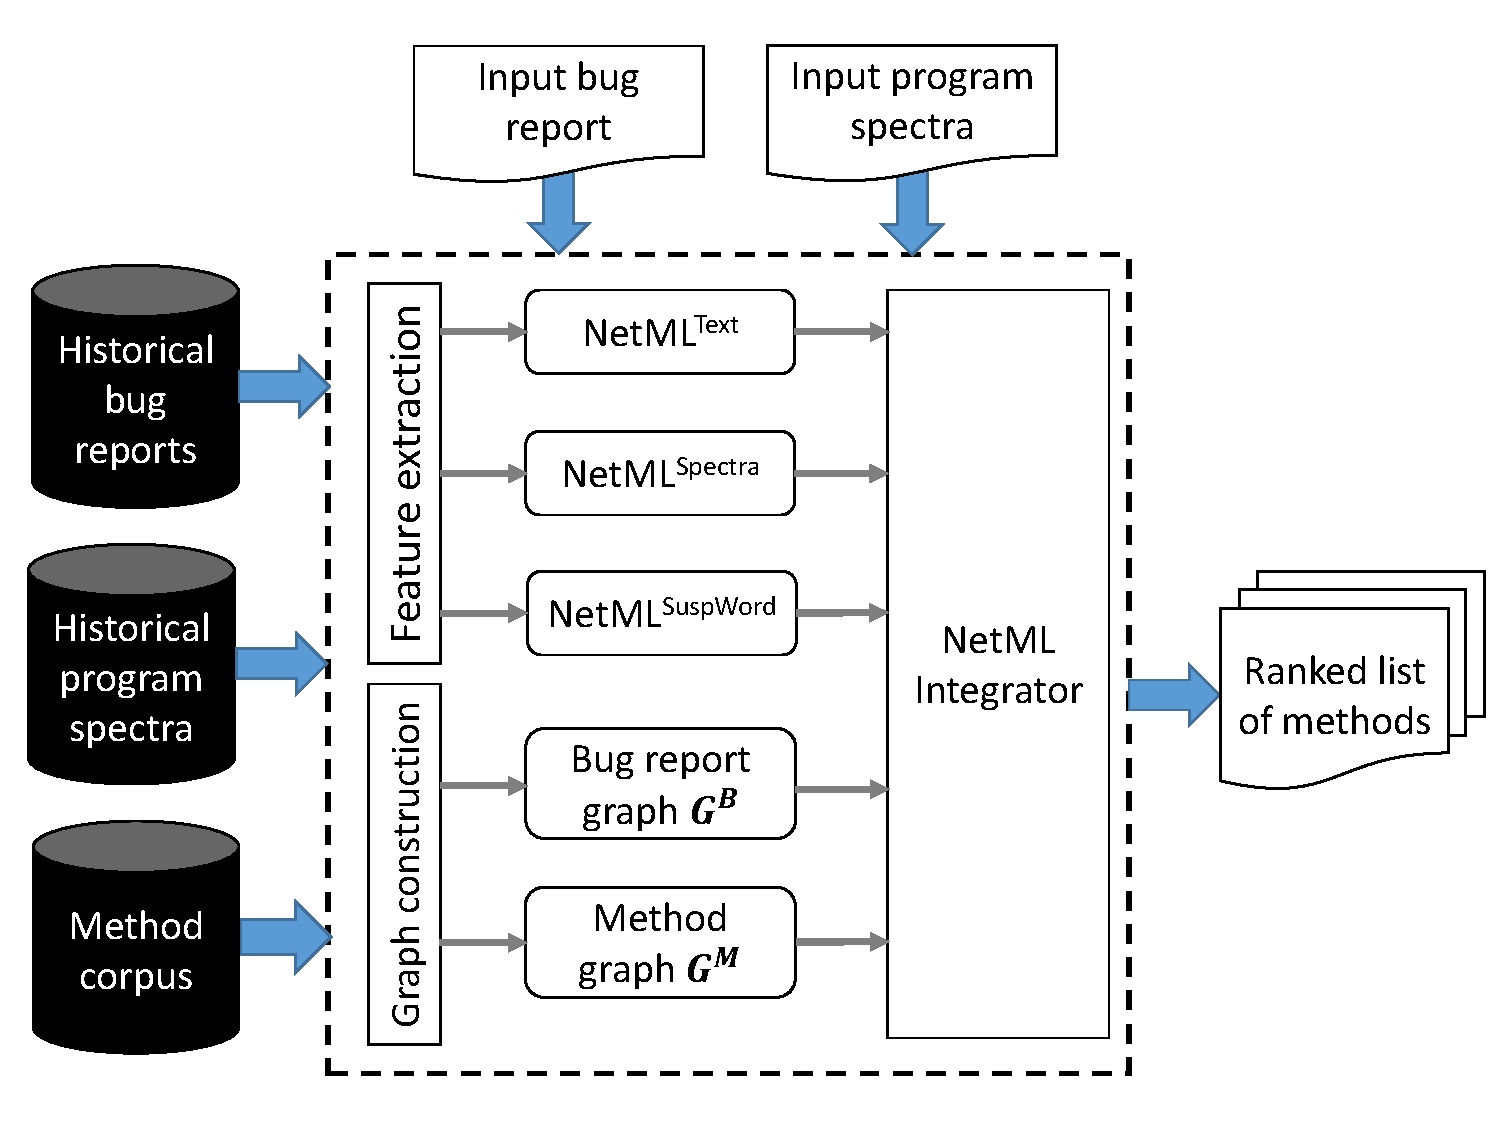
\includegraphics[width=0.5\textwidth]{netml_framework}
\caption{The proposed NetML framework}
\label{fig:framework}
\end{figure}

\subsection{Feature Extraction}
\label{subsec:feature}


The second component of the NetML framework is the feature extraction module, which generates features $\mathbf{X} = \{ x_{b,m.j} \}$ to be fed as inputs to the NetML integrator (see  Fig. \ref{fig:framework}). In line with our earlier AML work \cite{Le:2015:IRS:2786805.2786880}, for each bug report--method pair $(b,m)$, we compute a feature vector $\vec{x}_{b,m}$  that consists of three elements (i.e., $J = 3$):
\begin{align}
\vec{x}_{b,m} = \left[ \text{NetML}^\text{Text}_{b,m}, \text{NetML}^\text{Spectra}_{b, m}, \text{NetML}^\text{SuspWord}_{b,m} \right]
\end{align}
The three features are elaborated in turn below.



$\text{NetML}^\text{Text}_{b,m}$ makes use of the TF-IDF method~\cite{Ramos1999} to estimate the similarity between methods and bug reports. In particular, given a method $m$ and a bug report $b$, $\text{NetML}^\text{Text}_{b,m}$ computes the cosine similarity between the TF-IDF representation of the bug report text and that of the method codes, which is akin to the IR-based bug localization method (cf. Section~\ref{sec.IR-based}). That is, $\text{NetML}^\text{Text}_{b,m}$ is given by:
\begin{align}
\text{NetML}^\text{Text}_{b,m} = sim(b,m)	
\end{align}
where $sim(b,m)$ is the cosine similarity as defined in (\ref{eqn:cosine_sim}).


$\text{NetML}^\text{Spectra}_{b, m}$ processes only the program spectra information using a spectrum-based bug localization technique described in Section~\ref{sec.spectrum-based}. Given a program spectra $p$ corresponding to bug report $b$ and a method $m$, $\text{NetML}^\text{Spectra}_{b, m}$ gives a score that quantifies how suspicious  $m$ is given $p$. By default, $\text{NetML}^\text{Spectra}_{b, m}$ uses the Tarantula method as described in Section \ref{sec.spectrum-based} (cf. equation (\ref{eqn:tarantula})):
\begin{align}
\text{NetML}^\text{Spectra}_{b, m} = Tarantula(m, p)
\end{align}


Finally, $\text{NetML}^\text{SuspWord}_{b,m}$ processes both bug reports and program spectra, and computes the suspiciousness scores of words to rank different methods. It breaks a method into its constituent words, computes the suspiciousness scores of these words, and then aggregates these scores back in order to arrive at the suspiciousness score of the method. Given a bug report $b$, a program spectra $p$, and a method $m$ in a corpus $C$, $\text{NetML}^\text{SuspWord}_{b,m}$ measures how suspicious $m$ is considering $b$ and $p$,  as follows: %Thus, NetML$^\text{SuspWord}$ involves three basic steps: mapping of methods to words, computing word suspiciousness, and composing word suspiciousness into method suspiciousness. 
\begin{align}
&\text{NetML}^\text{SuspWord}_{b,m} = \text{NetML}^\text{Spectra}_{b, m} \times \\
%\text{SS}_{\text{method}}(m,p)\nonumber \times\\
&\frac{\sum\limits_{w\in b \cap m} \text{SSTFIDF}(w,p,b,C)\times \text{SSTFIDF}(w,p,m,C)}{\sqrt{\sum\limits_{w \in b} \text{SSTFIDF}(w,p,b,C)^2} \times \sqrt{\sum\limits_{w \in m} \text{SSTFIDF}(w,p,m,C)^2}}
\label{eq:sum_vsm_susp}
\end{align}
where 
%$\text{SS}_{\text{method}}(m,p)$ is the suspiciousness scores of a method, which by default uses  the same score as the NetML$^{spectra}(m)$ component, and 
$\text{SSTFIDF}(w,p,b,C)$ is the weight of a word $w$ in document (i.e., bug report or method) $d$ with corpus $C$ given program spectra $p$:
\begin{align}
\text{SSTFIDF}(w,p,d,C) = &\text{SS}_{\text{word}}(w,p)\times \ln(f(w,d)+1) \nonumber\\
&\times \ln\frac{|C|}{|{d_i\in C : w \in d_i }|}
\end{align}
where $\text{SS}_{\text{word}}(w,p)$ is the suspiciousness score of a word $w$:
\begin{align}
\text{SS}_{\text{word}}(w,p) &= \frac{\frac{|EF(w,p)|}{|p.FAIL|}}{\frac{|EF(w,p)|}{|p.FAIL|}+\frac{|ES(w,p)|}{|p.SUCCESS|}}
\label{eq:ss}
\end{align}
In the above equation, $EF(w,p)$ is the set of execution traces in $p.FAIL$ that contain a method in which the word $w$ appears, while $ES(w,p)$ is the set of execution traces in $p.SUCCESS$ that contain a method in which the word $w$ appears. Further details of all these components can be found in~\cite{Le:2015:IRS:2786805.2786880}.


%\recheck{Altogether, the three features that provide a multi-modal perspective on the degree of relevancy between a bug report and a method, are then sent to the NetML integrator in order to produce a ranked list of methods (given a bug report $b$ (cf. Fig.~\ref{fig:framework}).}

%The $\text{NetML}^\text{Text}_{b,m}$ and $\text{NetML}^\text{Spectra}_{m}$  components reuse techniques proposed in prior works which are described in Section~\ref{sec.prelim}. In the next subsections, we briefly describe the components namely NetML$^\text{SuspWord}$ and the network-clustered integrator component.
%
%Parnin and Orso {highlighted} that ``future research could also investigate ways to automatically suggest or highlight terms that might be related to a failure''~\cite{ParninO11}, however they did not propose a concrete solution. We use Parnin and Orso's observation, which highlights that some words are indicative to the location of a bug, as a starting point to design our NetML$^\text{SuspWord}$ component. \iffalse NetML$^\text{SuspWord}$ component is designed based on this observation made by Parnin and Orso which highlights that some words are indicative to the location of a bug.\fi
%This component breaks down a method into its constituent words, computes the suspiciousness scores of these words, and composes these scores back to result in the suspiciousness score of the method. The process is analogous to a machine learning or classification algorithm that breaks a data point into its constituent features, assign weights or importance to these features, and use these features, especially important ones, to assign likelihood scores to the data point. The component works in three steps: mapping of methods to words, computing word suspiciousness, and composing word suspiciousness into method suspiciousness. We describe each of these steps in the following sections. 
%
%% component takes in a spectra and a bug report to compute the suspiciousness scores of words. The suspicious words are then used to rank methods. Different from the $AML^{SPECTRA}$ component that directly computes the suspiciousness scores of methods, this
%
%\subsubsection{Mapping of Methods to Words}
%In this step, we map a method to its constituent words. For every method, we extract the following textual contents including: (1) The name of the method, along with the names of its parameters, and identifiers contained in the method body; (2) The name of the class containing the method, and the package containing the class; (3) The comments that are associated to the method (e.g., the Javadoc comment of that method, and the comments that appear inside the method), and comments that appear in the class (containing the method) that are not associated to any particular method.
%
%After we have extracted the above textual contents, we apply the text pre-processing step described in Section~\ref{sec.prelim}. At the end of this step, for every method we map it to a set of pre-processed words. Given a method $m$, we denote the set of words it contains as $words(m)$.
%
%\subsubsection{Computing Word Suspiciousness}
%We compute the suspiciousness score of a word by considering the program elements that contain the word. Let us denote the set of all failing execution traces in spectra $p$ as $p.F$ and the set of all successful execution traces as $p.S$. To compute the suspiciousness scores of a word $w$ given spectra $p$, we define several sets:
%%\begin{eqnarray}
%%EF(w,p) = \{t \in p.F | \exists {m\in t}~s.t.~w\in words(m)\}\footnotemark[1]\nonumber\\
%%NF(w,p) = \{t \in p.F | \not\exists {m\in t}~s.t.~w\in words(m)\}\nonumber\\
%%ES(w,p) = \{t \in p.S | \exists {m\in t}~s.t.~w\in words(m)\}\nonumber\\
%%NS(w,p) = \{t \in p.S | \not\exists {m\in t}~s.t.~w\in words(m)\}\nonumber
%%\end{eqnarray}
%\begin{align*}
%EF(w,p) &= \{t \in p.F | \exists {m\in t}~s.t.~w\in words(m)\}\nonumber\\
%%NF(w,p) &= \{t \in p.F | \not\exists {m\in t}~s.t.~w\in words(m)\}\nonumber\\
%ES(w,p) &= \{t \in p.S | \exists {m\in t}~s.t.~w\in words(m)\}\nonumber
%%NS(w,p) &= \{t \in p.S | \not\exists {m\in t}~s.t.~w\in words(m)\}\nonumber
%\end{align*}
%The set $EF(w,p)$ is the set of execution traces in $p.F$ that contain a method in which the word $w$ appears. The set $ES(w,p)$ is the set of execution traces in $p.S$ that contain a method in which the word $w$ appears. Based on these sets, we can compute the suspiciousness score of a word $w$ using a formula similar to Tarantula as follows:
%\begin{equation}
%\text{SS}_{\text{word}}(w,p)=\frac{\frac{|EF(w,p)|}{|p.FAIL|}}{\frac{|EF(w,p)|}{|p.FAIL|}+\frac{|ES(w,p)|}{|p.SUCCESS|}}
%\label{eq:ss}
%\end{equation}
%
%Using the above formula, words that appear more often in methods that are executed in failing execution traces are deemed to be more suspicious than those that appear less often in such methods.
%
%%The set $NF(w,p)$ is the set of execution traces in $p.F$ that do not contain a method in which the word $w$ appears. The set $NS(w,p)$ is the set of execution traces in $p.S$ that do not contain a method in which the word $w$ appears.
%
%\subsubsection{Computing Method Suspiciousness}
%To compute a method $m$'s suspiciousness score, we compute the textual similarity between $m$ and the input bug report $b$, and consider the appearances of $m$ in the input program spectra $p$. In the textual similarity computation, the suspiciousness of words are used to determine their weights.
%
%First, we create a vector of weights that represents a bug report and another vector of weights that represents a method. Each element in a vector corresponds to a word that appears in either the bug report or the method. The weight of a word $w$ in document (i.e., bug report or method) $d$ of method corpus $C$ considering program spectra $p$ is:
%\begin{align*}
%\text{SSTFIDF}(w,p,d,C)=&\text{SS}_{\text{word}}(w,p)\times \ln(f(w,d)+1)\\
%&\times \ln\frac{|C|}{|{d_i\in C : w \in d_i }|}
%\end{align*}
%In the above formula, $\text{SS}_\text{word}(w,p)$ is the suspiciousness score of word $w$ computed by Equation~\ref{eq:ss}, $f(w,d)$ is the number of times word $w$ appears in document $d$, and $d_i \in C$ means document $d_i$ is in the set of document $C$. Similarly, $w \in d_i$ means word $w$ belongs to document $d_i$. The above formula considers the weight of a word based on its suspiciousness, and well-known information retrieval metrics: term frequency (i.e., $\ln(f(w,d)+1)$) and inverse document frequency (i.e., $\ln\frac{|C|}{|{d_i\in C : w \in d_i }|}$).
%
%After the two vectors of weights of method $m$ and bug report $b$ are computed, we compute the suspiciousness score of the method $m$ by computing the cosine similarity of these two vectors multiplied by a weighting factor. The formula to compute this score is as follows:
%\begin{align}
%&\text{AML}^\text{SuspWord}(b,p,m,C)=\text{SS}_{\text{method}}(m,p)\nonumber \times\\
%&\frac{\sum\limits_{w\in b \cap m} \text{SSTFIDF}(w,p,b,C)\times \text{SSTFIDF}(w,p,m,C)}{\sqrt{\sum\limits_{w \in b} \text{SSTFIDF}(w,p,b,C)^2} \times \sqrt{\sum\limits_{w \in m} \text{SSTFIDF}(w,p,m,C)^2}}
%\label{eq:sum_vsm_susp}
%\end{align}
%Here we use $\text{SS}_\text{method}(m,p)$ that computes the suspiciousness score of method $m$ considering program spectra $p$ as the weighting factor. This can be computed by various spectrum-based bug localization tools. By default, we use the same fault localization tool as the one used in $\text{NetML}^\text{Spectra}_{m}$ component. With this, NetML$^\text{SuspWord}$ integrates both macro view of method suspiciousness (which considers direct execution of a method in the failing and correct execution traces) and micro view of method suspiciousness (which considers the executions of its constituent words in the execution traces).

\subsection{Graph Construction}
\label{subsec:graph}

The final component of the NetML framework is the graph construction module, which serves to compute the similarity graphs among bug reports and methods, to be used in the K-nearest neighbor retrieval as well as the network Lasso regularization. In this work, we define the bug report similarity graph $\mathcal{G}_B$ as comprising edge weights that reflect the textual similarity between two bug reports. For a pair of bug reports $b$ and $b'$, we define the edge weight $e_{b.b'}$ as:
\begin{align}
\label{eqn:edge_b}
e_{b,b'} = sim(b, b')
\end{align}
where $sim(b,b')$ is the cosine similarity between the TF-IDF weights of the textual descriptions of $b$ and $b'$, as per (\ref{eqn:cosine_sim}).


Similarly, the method similarity graph $\mathcal{G}_M$ comprises a set of edge weights $e_{m,m'}$ that reflect the textual similarity between two methods $m$ and $m'$. This is given by:
\begin{align}
\label{eqn:edge_m}
e_{m,m'} = sim(m, m')
\end{align}
where $sim(b,b')$ is the cosine similarity between the TF-IDF representations of the source codes of $m$ and $m'$.


\subsection{Integrator Model}
\label{sec.generalized_adaptive}

%As we mention in Section~\ref{sec.intro}, \underline{A}daptive \underline{M}ulti-modal bug \underline{L}ocalization (AML)~\cite{Le:2015:IRS:2786805.2786880} remains two main issues. Firstly, AML only proposes the concept of latent parameter for bug reports. In particular, every method $m$ share the same bug report parameter when estimating the suspiciousness scores of $m$, without considering the method parameter. Hence, AML may not capture the properties of different methods, leading to limit its effectiveness of detecting bug. Secondly, the latent paprameter of each bug report is learned independently of other bug report, without exploiting the clustering and/or similarity properties of different bug reports and methods. In practice, some bug reports as well as methods are similar to other bug reports/methods. However, AML simply ignores the relationship between bug reports and methods. 

The new integrator model proposed in this work characterizes the relevancy of a method $m$ to a given bug report $b$ as an interaction between two types of latent parameters, namely: \emph{latent bug report parameters} $\vec{u}_b = [u_{b,1}, \ldots, u_{b,j}, \ldots, u_{b,J}]$ and \emph{latent method parameters} $\vec{v}_m = [v_{m,1}, \ldots, v_{m,j}, \ldots, v_{m,J}]$, where $J$ is the total number of features. More specifically, the integrator model computes the relevancy score $\hat{f}_{b,m}$ as follows: 
%The first is to redefine the suspiciousness score of method $m$ given by bug reports $b$ as an interaction between a bug report’s parameter vector $\vec{u}_b$ and a method’s parameter vector $\vec{v}_m$. In particular, NetML 
%We propose \underline{N}etwork-clustered \underline{M}ulti-modal Bug \underline{L}ocalization (NetML) that involves two extensions. The first is to redefine the suspiciousness score of method $m$ given by bug reports $b$ as an interaction between a bug report’s parameter vector $\vec{u}_b$ and a method’s parameter vector $\vec{v}_m$, as follows: 
%The first is to redefine the function of suspiciousness score (see equation \ref{eqn:composite}) as an interaction between a bug report’s parameter vector $\vec{u}_b$ and a method’s parameter vector $\vec{v}_m$, as follows:
\begin{align}
\label{eq:aml_plus}
\hat{f}_{b,m} = \hat{f}(\vec{x}_{b,m}, \vec{u}_b, \vec{v}_m) = \sum_{j = 1}^{J} (u_{b,j} + v_{m,j}) x_{b,m,j}
\end{align}
where $\vec{x}_{b,m} = [x_{b,m,1}, \ldots, x_{b,m,j}, \ldots, x_{b,m,J}]$ is the feature vector corresponding to a bug report--method pair $(b, m)$.

It is worth mentioning that the above model constitutes a generalization of the AML integrator model that we previously developed~\cite{Le:2015:IRS:2786805.2786880}. In AML, the final relevancy score is computed based solely on the latent bug report parameters, and this set of parameters is shared by all methods for a given bug report. On the other hand, the NetML integrator model accounts for not only the latent bug report parameters but also the latent method parameters. The addition of the latter parameters provides a greater degree of freedom/flexibility in quantifying the contribution of different methods to the localization of a given bug report.

%In light of these issues, we propose a new algorithm, namely \underline{N}etwork-clustered \underline{M}ulti-modal Bug \underline{L}ocalization (NetML). More specifically, NetML tries to addresses these two shortcomings by performing joint optimization of localization loss function and clustering of both bug reports and methods. Firstly, NetML integrates two sets of latent parameters (i.e., bug reports and methods) to localize bug more accurately. Secondly, NetML takes advantage of network Lasso regularization~\cite{Hallac:2015:NLC:2783258.2783313} to enforce similar bug reports as well as methods to have similar latent parameters. Thus, the proposed approaches may achieve a more effective bug localization. 
%
%In the following section, we firstly present a short introduction about network Lasso, and briefly explain our proposed algorithm, i.e., NetML. 
%
%
%%Firstly, for each bug report $b$, a fixed parameter vector $\vec{\theta}_b = (\alpha, \beta, \gamma)$ is inferred for all methods $m$ (see Equation~\ref{eqn:composite}). 
%%In other words, every method $m$ shares the same parameter vector $\vec{\theta}_b$ when estimating the suspiciousness scores of $m$ according to bug report $b$ and program spectra $p$. In particular, each method $m$ not only considers the parameter of bug report $b$ but also share the parameter of method $m$. 
%%Therefore, Equation~\ref{eqn:composite} does not accurately reflect the suspiciousness score of method $m$ given bug report $b$ and program spectra $p$. Secondly, the parameter vector $\vec{\theta}_b$ of a bug report is learned independently of other bug report $b'$, without exploiting the clustering and/or similarity properties of different bug reports and methods. In practice, some bug reports as well as methods are similar to other bug reports/methods. However, the instance-wise loss function in equation \ref{eq:instance-wise-loss} ignores the relationship between the bug reports and the methods. In light of these issues, we proposed a new algorithm, namely generalized adaptive multi-modal bug localization, to tackle these problems in bug localization. 
%
%%Our proposed algorithm is inspired by network lasso \cite{Hallac:2015:NLC:2783258.2783313}. In the next sub section, I briefly present a short introduction about network lasso, then explain the proposed algorithm, i.e. \underline{G}eneralized \underline{A}daptive \underline{M}ulti-modal bug \underline{L}ocalization (AML*).
%
%\subsubsection{Network Lasso}\label{subsec:networklasso}
%
%Nowadays, convex optimization has become a popular way of modeling problems in many different fields (i.e., clock synchronization, smart power grids, state estimation, etc.). However, classical methods of convex analysis, relying on interior point methods~\cite{Renegar:2001:MVI:502968}, begin to fail due to a lack of scalability since datasets is getting larger and more intricate. The challenge of large-scale optimization lies in developing methods general enough to work well independent of the input, while being capable of scaling to the immense datasets that today’s applications require. In~\cite{Hallac:2015:NLC:2783258.2783313}, Hallac et al. proposed a network setting, namely network Lasso, that allows for simultaneous clustering and optimization on graph. In particular, given a graph $\mathcal{G}=(\mathcal{V}, \mathcal{E})$, where $\mathcal{V}$ is the vertex set and $\mathcal{E}$ is the edges of graph. The network Lasso problem is defined as following: 
%
%%Therefore, it is necessary to formulate general classes of convex optimization solvers, ones that can apply to a variety of interesting and relevant problems, and to develop algorithms for reliable and efficient solutions.
%
%%Network Lasso~\cite{Hallac:2015:NLC:2783258.2783313} is a generalization of the group lasso to a network setting that allows for simultaneous clustering and optimization on graphs. In~\cite{Hallac:2015:NLC:2783258.2783313}, Hallac et al. focused on optimization problem posed on graph. Given a graph $\mathcal{G}=(\mathcal{V}, \mathcal{E})$, where $\mathcal{V}$ is the vertex set and $\mathcal{E}$ is the edges of graph. The network lasso problem is defined as following: 
%\begin{align}
%\label{eq:network_lasso}
%	minimize \sum_{i \in \mathcal{V}}^{} f_i(\vec{x}_{b,m}) + \lambda \sum_{(j, k) \in \mathcal{E}}^{} w_{jk} \|x_j - x_k \|_{2}	
%\end{align}
%The variable are $x_1, \dots, x_n \in R^{p}$, where $n = |\mathcal{V}|$. $\vec{x}_{b,m} \in R^{p}$ is the variable at node $i$, $f_i$ is the cost function at node $i$, $w_{jk}$ is the relative weights among the edges $(j,k)$ of the network $\mathcal{G}$, and $\lambda$ is an overall parameter that scales the edge objectives relative to the node objectives. In order to solve the problem \ref{eq:network_lasso} in a distributed and scalable manner, which allows for guaranteed global convergence even on large graphs, the author based on the Alternating Direction Method of Multipliers (ADMM)~\cite{Parikh:2014:PA:2693612.2693613, Boyd:2011:DOS:2185815.2185816}. With ADMM, each individual component solves its own private objective function, passes this solution to its neighbors, and repeats the process until the entire network converges. 

\subsection{Objective Function}
\label{subsec:objective}

%The second extension takes advantage of network Lasso regularization~\cite{Hallac:2015:NLC:2783258.2783313} to enforce similar bug reports as well as methods to have similar latent parameters. Different from the original network Lasso that only deals with a single graph, our approach involves optimizing over two graphs simultaneously. Specifically, we consider a joint optimization over the bug similarity graph $\mathcal{G}^B=\{e_{b,b'}|(b, b') \in B\}$, and method similarity graph $\mathcal{G}^M=\{e_{m,m'}|(m, m') \in M\}$.

Based on the above model formulation, we devise an objective function that guides the learning process of our integrator model. Specifically, we consider a joint optimization of bug localization quality and clustering of similar bug reports and methods, expressed by the loss function $\mathcal{L}$:
\begin{align}
\label{eq:NL_lossfunc}
\mathcal{L} &= \mathcal{L}_\text{Entropy} + \mathcal{L}_\text{Ridge} + \mathcal{L}_\text{NetLasso}
\end{align}
This consists of three components:
\begin{align}
\label{eq:entropy}
\mathcal{L}_\text{Entropy} = & -\sum_{b \in \mathcal{B}} \sum_{m \in \mathcal{M}} w_{b,m} \left[y_{b,m} \ln(\sigma(\hat{f}_{b,m})) \right. \nonumber\\
	& + \left. (1 - y_{b,m}) \ln(1- \sigma(\hat{f}_{b,m})) \right] \\
\label{eq:ridge}
\mathcal{L}_\text{Ridge} = &\frac{\alpha}{2} \sum_{j=1}^{J} \left[\sum_{b \in \mathcal{B}} u_{b,j}^2 + \sum_{m \in \mathcal{M}} v_{m,j}^2 \right] \\
\label{eq:netlasso}
\mathcal{L}_\text{NetLasso} = & \frac{\beta}{2} \sum_{j=1}^{J} \left[ \sum_{(b, b') \in \mathcal{G}^B}^{} e_{b, b'} (u_{b,j} - u_{b', j})^2 \right. \nonumber\\ 
	& + \left. \sum_{(m, m') \in \mathcal{G}^M}^{} e_{m, m'} (u_{m,j} - u_{m', j})^2 \right]
\end{align}
where $\mathcal{B}$ and $\mathcal{M}$ are the sets of bug reports and methods respectively, $y_{b,m}$ is a binary label that indicates whether method $m$ is relevant to bug report $b$ ($y_{b,m} = 1$) or not ($y_{b,m} = 0$), and $\sigma(\hat{f}_{b,m}) = \frac{1}{1 + \exp(-\hat{f}_{b,m})}$ is the logistic function \cite{Collins:2002:LRA:599615.599689}. Also, $w_{b,m}$ denotes the instance weight of a bug report--method pair $(b,m)$, while $e_{b,b'}$ and $e_{m,m'}$ are the edge weights reflecting the degree of similarity between two bug reports $b$ and $b'$, and two methods $m$ and $m'$, respectively. Finally, $\alpha > 0$ and $\beta > 0$ are the user-defined parameters that control the strength of the ridge and network Lasso regularization, respectively.

Note that $\mathcal{L}_\text{Entropy}$ refers to the so-called cross-entropy loss \cite{Murphy:2012:MLP:2380985}, which provides an error measure of the bug localization process. Here $\mathcal{L}_\text{Entropy}$ can be interpreted as the discrepancy between the probability distribution of the predictive model $\hat{f}_{b,m}$ and that of the true label $y_{b,m}$ \cite{Murphy:2012:MLP:2380985}. We also introduce the instance weight\footnote{An instance refers to a specific bug report--method pair $(b,m)$} $w_{b,m}$ in (\ref{eq:entropy}) to cater for the extremely \emph{skewed} distribution of the relevant vs. irrelevant methods for a given bug report, which is a major challenge in bug localization process. That is, the number of relevant (faulty) methods is much smaller than that of irrelevant (non-faulty) ones. To address this, we configure $w_{b,m}$ in such a way that imposes a greater penalty for relevant instances being incorrectly predicted/classified than that for irrelevant ones. Specifically, we set $w_{b,m}$ as:
\begin{align}
w_{b,m} =
\begin{cases}
    \frac{1}{N_\text{faulty}},     & \text{if } y_{b,m} = 1\\
    \frac{1}{N - N_\text{non-faulty}}, & \text{if } y_{b,m} = 0
\end{cases}
\end{align}
where $N$ is the total number of instances observed in the historical data, and $N_\text{faulty}$ is the number of faulty instances.

Meanwhile, the ridge regularization $\mathcal{L}_\text{Ridge}$ serves to penalize large values of the latent parameters \cite{Murphy:2012:MLP:2380985}, which in turn helps mitigate the risk of data overfitting. From a probabilistic perspective, this corresponds to the Gaussian prior distribution for the latent parameters $u_{b,j}$ and $v_{m,j}$, with zero mean and inverse variance of $\alpha$~\cite{Le:2015:IRS:2786805.2786880}. Finally, $\mathcal{L}_\text{NetLasso}$ refers to the network Lasso regularization \cite{Hallac:2015:NLC:2783258.2783313}, which enforces clustering of the latent parameters of bug reports and methods. The intuition is straightforward---the more similar two bug reports or two methods are (as quantified by $e_{b,b'}$ and $e_{m,m'}$), the closer their latent parameters $\vec{u}_b$ and $\vec{v}_m$ should be. This combination of $\mathcal{L}_\text{Entropy}$, $\mathcal{L}_\text{Ridge}$ and $\mathcal{L}_\text{NetLasso}$ facilitates a robust model that can simultaneously optimize the bug localization quality and cluster the latent parameters of similar bug reports and methods.

Next, in order to minimize the joint loss $\mathcal{L}$, we employ a Newton method \cite{doi:10.1137/1.9780898718898} that is derived from a second-order Taylor series expansion of the loss function $\mathcal{L}$:
\begin{align}
\label{eq:newton}
	\mathcal{L}(\theta) = \mathcal{L}(\theta_0) + \triangledown \mathcal{L}(\theta_0) (\theta - \theta_0) + \frac{\triangledown^2 \mathcal{L}(\theta_0)}{2} (\theta - \theta_0)^2
\end{align}
The minima of $\mathcal{L}$ can be obtained by taking the partial derivative of $\mathcal{L}(\theta)$ and equating it to zero:
\begin{align}
0 &= \triangledown \mathcal{L}(\theta_0) + \triangledown^2 \mathcal{L}(\theta_0) (\theta - \theta_0) \nonumber\\
\theta &= \theta_0 - \frac{\triangledown \mathcal{L}(\theta_0)}{\triangledown^2 \mathcal{L}(\theta_0)}
\end{align}
If we take $\theta_0$ as the old estimate of $u_{b,j}$ or $v_{m,j}$, this leads to the following update formulae:
\begin{align}
\label{eqn:update_u}
u_{b,j} &\leftarrow u_{b,j} - \frac{ \triangledown \mathcal{L}(u_{b,j}) }{ \triangledown^2 \mathcal{L}(u_{b,j}) } \\
\label{eqn:update_v}
v_{m,j} &\leftarrow v_{m,j} - \frac{ \triangledown \mathcal{L}(v_{m,j}) }{ \triangledown^2 \mathcal{L}(v_{m,j}) }
\end{align}

In turn, we need to compute the first and second derivatives of each latent parameter $u_{b,j}$ and $v_{m,j}$. For the latent bug report parameter $u_{b,j}$, the first and second derivatives are respectively given by:
\begin{align}
\label{eqn:grad_u}
\triangledown \mathcal{L}(u_{b,j}) &= \sum_{m \in \mathcal{M}} \left[ w_{b,m} (\sigma(\hat{f}_{b,m}) - y_{b,m}) x_{b,m,j} \right] \nonumber \\
&+ \alpha u_{b,j} + \beta \sum_{b'} \left[ e_{b,b'} \left( u_{b,j} - u_{b',j} \right) \right] \\
\label{eqn:hess_u}
\triangledown^2 \mathcal{L}(u_{b,j}) &= \sum_{m \in \mathcal{M}} \left[ w_{b,m} \sigma(\hat{f}_{b,m}) ( 1 - \sigma(\hat{f}_{b,m}) ) x_{b,m,j}^2 \right] \nonumber \\
&+ \alpha + \beta \sum_{b'} e_{b,b'}
\end{align}
Similarly, we can compute the first and second derivatives w.r.t each latent method parameter $v_{m,j}$ as:
\begin{align}
\label{eqn:grad_v}
\triangledown \mathcal{L}(v_{m,j}) &= \sum_{b \in \mathcal{B}} \left[ w_{b,m} (\sigma(\hat{f}_{b,m}) - y_{b,m}) x_{b,m,j} \right] \nonumber \\
& + \alpha v_{m,j} + \beta \sum_{m'} \left[ e_{m,m'} \left( v_{m,j} - v_{m',j} \right) \right] \\
\label{eqn:hess_v}
\triangledown^2 \mathcal{L}(v_{m,j}) &= \sum_{b \in \mathcal{B}} \left[ w_{b,m} \sigma(\hat{f}_{b,m}) ( 1 - \sigma(\hat{f}_{b,m})) x_{b,m,j}^2 \right] \nonumber \\
& + \alpha + \beta \sum_{m'} e_{m,m'}
% \label{eqn:grad_v}
% \triangledown \mathcal{L}(v_{m,j}) &= \sum_{b \in \mathcal{B}} \left[ (\sigma(\hat{f}_{b,m}) - y_{b,m}) u_{b,j} x_{b,m,j} \right] + \alpha v_{m,j} + \beta \sum_{m'} \left[ e_{m,m'} \left( v_{m,j} - v_{m',j} \right) \right] \\
% \label{eqn:hess_v}
% \triangledown^2 \mathcal{L}(v_{m,j}) &= \sum_{b \in \mathcal{B}} \left[ \sigma(\hat{f}_{b,m}) ( 1 - \sigma(\hat{f}_{b,m})) u_{b,j}^2 x_{b,m,j}^2 \right] + \alpha + \beta \sum_{m'} e_{m,m'}
\end{align}

\begin{algorithm*}[!ht]
	\begin{algorithmic}[1]
		\Require
		    \Statex Set of $K$ relevant historical bug reports $\mathcal{B}_K$ (i.e.,  $|\mathcal{B}_K| = K$)
			\Statex Set of all methods $\mathcal{M}$, where $|\mathcal{M}| = M$
		    \Statex New bug report query $b^*$ along with its features $\mathbf{X}_{b^*} = \{ x_{b^*,m,j} \} \in \mathbb{R}^{1 \times M \times J}$
			\Statex Historical features $\mathbf{X} = \{ x_{b,m,j} \} \in \mathbb{R}^{K \times M \times J}$
			\Statex Historical labels $\mathbf{Y} = \{ y_{b,m} \} \in \mathbb{R}^{K \times M}$
			\Statex Bug report similarity graph $\mathcal{G}_B$, represented by the adjacency matrix $\mathbf{E}_B = \{ e_{b,b'} \}$
			\Statex Method similarity graph $\mathcal{G}_M$, represented by the adjacency matrix $\mathbf{E}_M = \{ e_{m,m'} \}$
		\Ensure 
		    \Statex Relevancy scores $\hat{f}_{b^*,m} \in \mathbb{R}^{1 \times M}$ of the new bug report $b^*$ to all methods $m$
			\Statex Latent bug report parameters $\mathbf{U} = \{ u_{b,j} \} \in \mathbb{R}^{(K + 1) \times J}$ 
			\Statex Latent method parameters $\mathbf{V} = \{ v_{m,j} \} \in \mathbb{R}^{M \times J}$ 
		\Statex \hrulefill
		\State Compute the union set of bug reports $\mathcal{B} \leftarrow \mathcal{B}_K \cup \{ b^* \}$
		\State Initialize all latent parameters $u_{b,j} \leftarrow 0$ and $v_{m,j} \leftarrow 0$, $\forall b \in \mathcal{B}, m \in \mathcal{M}, j \in \{ 1,\ldots,J \}$
		\State Precompute all constant terms $q_b \leftarrow \sum_{b'} e_{b,b'}$ and $q_m \leftarrow \sum_{m'} e_{m,m'}$, $\forall b \in \mathcal{B}, m \in \mathcal{M}$
		\State Compute the bug probabilities $\sigma(\hat{f}_{b,m})$ for all $(b,m)$ pairs via equation (\ref{eq:aml_plus})
		\State $\mathcal{L}_\text{curr} \leftarrow -\sum_{b} \sum_{m} w_{b,m} \big[ y_{b,m} \ln \big( \sigma(\hat{f}_{b,m}) \big) + \big( 1 - y_{b,m} \big) \ln \big(1 - \sigma(\hat{f}_{b,m}) \big) \big]$
		\Repeat 
		\State $\mathcal{L}_\text{prev} \leftarrow \mathcal{L}_\text{curr}$
		\For {each $j \in \{ 1,\ldots,J \}$}
		\State \textbf{/* Update the latent bug report parameters $u_{b,j}$ */}
		\For {each $b \in \mathcal{B}$}
		\State $p_{b} \leftarrow \sum_{b'} e_{b,b'} u_{b',j}$
		\EndFor
		\For {each $b \in \mathcal{B}$}
		\State $u_\text{numer} \leftarrow \sum_m \big[ w_{b,m} (\sigma(\hat{f}_{b,m}) - y_{b,m}) x_{b,m,j} \big] + \beta \big[ u_{b,j} q_b - p_{b} \big] + \alpha u_{b,j}$
		\State $u_\text{denom} \leftarrow \sum_m \big[ w_{b,m} \sigma(\hat{f}_{b,m}) (1 - \sigma(\hat{f}_{b,m})) x_{b,m,j}^2 \big] + \beta q_b + \alpha$
		\State $u_{b,j} \leftarrow u_{b,j} - \eta \left( \frac{u_\text{numer}}{u_\text{denom}} \right)$
		\EndFor
		\State \textbf{/* Update the latent method parameters $v_{m,j}$ */}
		\For {each $m \in \mathcal{M}$}
		\State $p_{m} \leftarrow \sum_{m'} e_{m,m'} v_{m',j}$
		\EndFor
		\For {each $m \in \mathcal{M}$}
		\State $v_\text{numer} \leftarrow \sum_b \big[ w_{b,m} (\sigma(\hat{f}_{b,m}) - y_{b,m}) x_{b,m,j} \big] + \beta \big[ v_{m,j} q_m - p_{m} \big] + \alpha v_{m,j}$
		\State $v_\text{denom} \leftarrow \sum_b \big[ w_{b,m} \sigma(\hat{f}_{b,m}) (1 - \sigma(\hat{f}_{b,m})) x_{b,m,j}^2 \big] + \beta q_m + \alpha$
		\State $v_{m,j} \leftarrow v_{m,j} - \eta \left( \frac{v_\text{numer}}{v_\text{denom}} \right)$
		\EndFor
		\EndFor
		\State Compute the updated bug probabilities $\sigma(\hat{f}_{b,m})$ via equation (\ref{eq:aml_plus})
		\State $\mathcal{L}_\text{curr} \leftarrow -\sum_{b} \sum_{m} w_{b,m} \big[ y_{b,m} \ln \big( \sigma(\hat{f}_{b,m}) \big) + \big( 1 - y_{b,m} \big) \ln \big(1 - \sigma(\hat{f}_{b,m}) \big) \big]$
		\State $\eta \leftarrow
		\begin{cases}
		\frac{\eta}{2},   & \text{if } \mathcal{L}_\text{curr} > \mathcal{L}_\text{prev}\\
		\min(1, 2 \eta),  & \text{otherwise}
		\end{cases}$
		\Until $T_{max}$ iterations
		\State Compute the relevancy scores $\hat{f}_{b^*,m}$ using equation (\ref{eq:aml_plus})
	\end{algorithmic}
	\caption{Adaptive learning of the NetML integrator}
	\label{alg:network_lasso}
\end{algorithm*}


% \begin{algorithm}
% 	\begin{algorithmic}[1]
% 		\Require Matrix $X \in \mathbb{R}^{B \times M \times 3}$, where $B$ and $M$ are the number of bug reports and methods in our training data. Bug reports graph $\mathcal{G}^B=\{e_{b,b'}|(b, b') \in B\}$, , where $e_{b,b'}$ represents textual similarity between $b$ and $b'$.
% 		\State folds $\leftarrow$ cross\_validation($\mathcal{G}^B.vertex$)
% 		\For {\textit{test} in folds}
% 		\State $B_{test}$ $\leftarrow$ $\mathcal{G}^B[test]$
% 		\For {each $b \in B_{test}$ }
% 		\State Finding top-K most similarity bug reports of $b$
% 		\State Construct matrix $X_{train} \in {B_{topK} \times M \times 3}$
% 		\State Calling Algorithm~\ref{alg:network_lasso} for matrix $X_{train}$ with default parameters
% 		\State Predict all methods given by particular bug report $b$
% 		\EndFor
% 		\EndFor
% 	\end{algorithmic}
% 	\caption{Prediction procedure for localize bug report}
% 	\label{alg:prediction}
% \end{algorithm}

%The two graphs are respectively represented using the adjacency matrices $\mathbf{E}_{B} = \{ e_{b,b'} \}$ and $\mathbf{E}_M = \{ e_{m,m'} \}$.

Finally, the update formula for $u_{b,j}$ can be obtained by substituting equation (\ref{eqn:grad_u}) and (\ref{eqn:hess_u}) into equation (\ref{eqn:update_u}). Likewise, we can substitute (\ref{eqn:grad_v}) and (\ref{eqn:hess_v}) into (\ref{eqn:update_v}) to arrive at the update formula for $v_{m,j}$. To learn the latent parameters, we use a \emph{Newton method} that updates the parameters on a per-feature $j$ basis. This will be elaborated in Section \ref{sec:learning}.
%Starting from a random initial values of $u_{b,j}$ and $v_{m,j}$, we first update $u_{b,j}$ by assuming that all $v_{m,j}$ are fixed. We then alternate by updating $v_{m,j}$ with all $u_{b,j}$ assumed to be fixed.

\subsection{Adaptive Learning}
\label{sec:learning}

Algorithm \ref{alg:network_lasso} summarizes the adaptive learning procedure of the NetML integrator for computing the relevancy scores of a new bug report (i.e., a new query) to different methods (i.e., documents). Given a new bug report $b^*$, the set of $K$ relevant bug reports $\mathcal{B}_K$ in the historical data,  the set of all methods $\mathcal{M}$, and the similarity graphs $\mathcal{G}_B$ and $\mathcal{G}_M$, the learning procedure appends $b^*$ into $\mathcal{B}_K$ and then updates the latent parameters on a per-feature basis. That is, for each feature $j$, it performs Newton updates on the latent bug report parameters $u_{b,j}$ (steps 14--16) and latent method parameters $v_{m,j}$ (steps 23--25), in accordance with equations (\ref{eqn:update_u}) and (\ref{eqn:update_v}) respectively. The procedure is repeated until a maximum iteration $T_{max}$ is reached. Afterwards, the final prediction score $\hat{f}_{b^*,m}$ of the new bug report $b^*$ for each method $m$ is computed via equation (\ref{eq:aml_plus}).

Note that the selection of relevant bug report set $B_K$ is based on the $K$-nearest neighbor retrieval from the bug report similarity graph $\mathcal{G}_B$, as follows:
\begin{align}
\mathcal{B}_K = \text{Top}_K( \{ e_{b^*, b} \mid \forall b \neq b^* \} )
\end{align}
where $\text{Top}_K$ is a function that returns bug reports with the highest similarity $e_{b^*, b}$ to the query bug report $b^*$. The calculation of the similarity graphs is based on the VSM model and will be further described in Section \ref{subsec:graph}.

It is also worth mentioning that the magnitude of the Newton update is downscaled by an adaptive learning rate $\eta$ (where $0 < \eta \leq 1$). We introduce this scaling factor as a way to address the problem of \emph{overshooting} in Newton method \cite{Bank1981}, whereby the update $\frac{ \triangledown \mathcal{L}(u_{b,j}) }{ \triangledown^2 \mathcal{L}(u_{b,j}) }$ or $\frac{ \triangledown \mathcal{L}(v_{m,j}) }{ \triangledown^2 \mathcal{L}(v_{m,j}) }$ is overestimated---possibly by many orders of magnitude. This may lead to oscillations and sometimes divergence in the loss function. To alleviate this issue, we compare the loss function $\mathcal{L}$ before and after a Newton iteration (step 30), and then adjust $\eta$ accordingly depending on whether $\mathcal{L}$ increases or not. If it increases, then we reduce $\eta$ by half in order to dampen the update magnitude; otherwise, the value of $\eta$ gets doubled, up to a maximum limit of $1$.

For computational efficiency, we precompute the constant terms $q_b = \sum_{b'} e_{b,b'}$ and $q_m = \sum_{m'} e_{m,m'}$ before the Newton iterations begins. Additionally, during each Newton iteration, we have separate loops to compute the terms $\sum_{b'} e_{b,b'} u_{b',j}$ (step 11) and $\sum_{m'} e_{m,m'} v_{m',j}$ (step 20) for each feature $j$, prior to updating $u_{b,j}$ and $v_{m,j}$. The purpose is to make sure that, during the parameter updates (steps 14 and 23), the computation of $\sum_{b'} e_{b,b'} u_{b',j}$ in equation (\ref{eqn:update_u}) and $\sum_{m'} e_{m,m'} v_{m',j}$ in equation (\ref{eqn:update_v}) is based on the old parameter values from the previous iteration, and not affected by the ordering of $b$ or $m$ in the update loops.

%To predict method $m$ given by a new bug report $b$ and program spectra $p$, we base on a set of top-K historical fixed bugs in a training data that are the most similar to $b$. We find these top-K nearest neighbors by measuring the textual similarity of $b$ with training (historical) bug reports using the vector space model. These top-K nearest neighbors are used to construct our NetML model. Note that the prediction steps are similar to~\cite{Le:2015:IRS:2786805.2786880}.

%\recheck{Analyzing Algorithm \ref{alg:network_lasso} further, it can be observed that the overall time complexity of the adaptive learning procedure is in a linear order of the problem size. Specifically, for each new query $b*$ and given $K$-nearest bug reports and a total of $M$ methods, the (worst) time complexity would be $\mathcal{O}(T_{max}  \times K \times M \times J)$. Note that the problem size here corresponds to the size of the input features $\mathbf{X}$ in the historical data, i.e., $K \times M \times J$. Accordingly, for a total of $N$ new bug reports (queries), the total complexity would be $\mathcal{O}(N \times T_{max}  \times K \times M \times J)$. In practice, $K$ would be much smaller than the total number of bug reports in the historical data, while $T_{max}$ and $J$ are typically set to be small, fixed values. Hence, the overall computation time is moderate and can be scaled up to large dataset.} 

We additionally highlight that the loss function $\mathcal{L}$ is \emph{strictly convex}. This provides a nice theoretical guarantee that there is only one unique minimum in the loss function surface, and this minimum is globally optimal \cite{Renegar:2001:MVI:502968}. The convexity trait can be proven by looking at the curvatures (i.e., second derivatives) with respect to the latent bug report and method parameters, as per equations (\ref{eqn:hess_u}) and (\ref{eqn:hess_v}) respectively. Clearly, since $0 \leq \sigma(\hat{f}_{b,m}) \leq 1$, $w_{b,m}$, $x_{b,m,j}^2$, $e_{b,b'}$ and $e_{m,m'}$ are non-negative, while $\alpha$ and $\beta$ are positive, the curvatures will be positive. The positive curvatures correspond to the so-called \emph{positive definite} Hessian matrix---a well-known property of a strictly convex function \cite{Renegar:2001:MVI:502968}.








\section{Experiments }\label{sec.exp}
\section{Experiments }
\label{sec.exp}

In this section, we first describe the datasets and evaluation settings used in our experiments. We then present a list of research questions we want to address, and accordingly elaborate our experiment results. Finally, we discuss some potential threats to the validity of our approach.

% We then describe our evaluation metrics and experimental settings in Section~\ref{sec:metrics}. Next, we present the research questions in Section~\ref{sec:rqs}. The results of our experiments which answer the research questions are described in Sections~\ref{sec:rq1},~\ref{sec:rq2}~\&~\ref{sec:rq3}. Threats to validity are listed in Section~\ref{sec:threats}

\subsection{Dataset}\label{sec:dataset}

%To evaluate our approach, we use a dataset of 157 bugs from four popular software projects. The four projects are AspectJ~\cite{aspectj_link}, Ant~\cite{ant_link}, Lucene~\cite{lucene_link}, and Rhino~\cite{rhino_link}. All four projects are medium-large scale and implemented in Java. AspectJ, Ant, and Lucene contain more than 300 kLOC, while Rhino contains almost 100 kLOC. {\iffalse \color{red} (Duy: AspectJ uses BugZilla )These four projects use Jira as the issue tracking system, from which we retrieve their bug reports. Bissyande et al. found that in Jira bugs are generally well linked to commits that fix them~\cite{BissyandeTWLJR13}.\fi} Table~\ref{tab:dataset} describes detailed information of the four projects in our study.

To evaluate our approach, we use a dataset of 355 bugs from seven popular software projects. The seven projects are Ant~\cite{ant_link}, AspectJ~\cite{aspectj_link}, Lang~\cite{lang_link}, Lucene~\cite{lucene_link}, Math~\cite{math_link}, Rhino~\cite{rhino_link}, and Time~\cite{time_link}. All seven projects are medium-large scale and implemented in Java. Ant, AspectJ, and Lucene contain more than 300 kLOC. Math, Rhino, and Time contains almost 100 kLOC, while Lang only contains more than 50 KLOC. Ant, AspectJ, Lang, Lucene, Math, and Rhino projects use Jira as the issue tracking system, from which we retrieve their bug reports. Bissyande et al. found that in Jira bugs are generally well linked to commits that fix them~\cite{BissyandeTWLJR13}. Time uses Github as the issues tracking system, from which we collect their bug reports. Table~\ref{tab:dataset} describes detailed information of the seven projects in our study.

%
%\begin{table*}[t]
%	\center
%	\caption{Dataset Description}
%    \begin{tabular}{|c|c|c|c|c|c|c|c|c|c|c|c|}
%    \hline	
%     \multirow{2}{*}{\textbf{Project}}& \textbf{Number of}  &\multirow{2}{*}{\textbf{Study Perid}} & \multicolumn{3}{c|}{\textbf{Number of Methods}} & \multicolumn{3}{c|}{\textbf{Number of Failed Testcases}}  & \multicolumn{3}{c|}{\textbf{Number of Passed Testcases}}\\\cline{4-12}
%         ~ & \textbf{Bug Reports} & ~ & \textbf{Max} & \textbf{Median} & \textbf{Min} &\textbf{Max} & \textbf{Median} & \textbf{Min} & \textbf{Max} & \textbf{Median} & \textbf{Min} \\
%     \hline\hline
%    AspectJ & 41 & Mar. 2005 - Feb. 2007 & 28,083 & 13,908 & 10,683 & 9 & 1 & 1 & 818 & 803 & 52 \\\hline
%    Ant & 53 &  Dec. 2001 - Sept. 2013&10,451 &  9,655 & 8,345 &  8 & 1 & 1 & 1,554 & 1,237 & 575 \\\hline
%    Lucene & 37 & June 2006 - Jan. 2011 & 15,487 & 9,416 & 9,103 & 15 & 1 & 1 & 1,160 & 1,090 & 655 \\\hline
%	Rhino & 26 & Dec. 2007 - Dec. 2011 & 5,312 & 4,849 & 3,754 & 7 & 1 & 1 & 185~ & 104.5 & 111 \\\hline
%
%    \end{tabular}
%    \label{tab:dataset}
%\end{table*}

\begin{table}[t]
	\centering
	\caption{Dataset Description}
	%\scalebox{0.92}{
    \begin{tabular}{|l|c|c|r|}
    \hline
   \multirow{2}{*}{\textbf{Project}} &\multirow{2}{*}{\textbf{\#Bugs}}&{\multirow{2}{*}{\textbf{Time Period}}}& \textbf{Average}   \\
    ~       &             &                                   &\textbf{\# Methods}   \\ \hline
	\hline
	Ant       & 53                                          & 12/2001 -- 09/2013 & 9,624.66   \\ 
    AspectJ       & 41                                              & 03/2005 -- 02/2007                                   & 14,218.39   \\ 
%    \hline
     
%     \hline
Lang       &     65                                          & 	10/2002 -- 	04/2016 & 2,151.1  \\
    Lucene       & 37                                              & 06/2006 -- 01/2011                   & 10,220.14   \\
    Math       & 106                                              &  12/2004 --  03/2016& 4,792.3   \\ 
%    \hline
    Rhino       & 26                                                 &  12/2007 -- 12/2011                                   & 4,839.58   \\
    Time       & 27                                                 &                      05/2004 -- 03/2017            & 4,083.5
    \\ \hline
    \end{tabular}
    %}
    \label{tab:dataset}
\end{table}

%The 41 AspectJ bugs are from the iBugs dataset which was collected by Dallmeier and Zimmermann~\cite{DallmeierZ07}. Each bug in the iBugs dataset comes with the code before the fix (pre-fix version), the code after the fix (post-fix version), and a set of test cases. The iBugs dataset contains more than 41 AspectJ bugs, but not all of them come with failing test cases. Test cases provided in the iBugs dataset are obtained from the various versions of the regression test suite that comes with AspectJ. The remaining 116 bugs from Ant, Lucene, and Rhino were collected by ourselves, following the procedure used by Dallmeier and Zimmermann~\cite{DallmeierZ07}. For each bug, we collected the pre-fix version, post-fix version, a set of successful test cases, and at least one failing test case. A failing test case is often included as an attachment to a bug report or committed along with the fix in the post-fix version. When a developer receives a bug report, he/she first needs to replicate the error described in the report~\cite{worksforme}. In this process, he is creating a failing test case. Unfortunately, not all test cases are documented and saved in the version control systems.

The 116 bugs from Ant, Lucene, and Rhino were collected by ourselves, following the procedure used by Dallmeier and Zimmermann~\cite{DallmeierZ07}. For each bug, we collected the pre-fix version, post-fix version, a set of successful test cases, and at least one failing test case. A failing test case is often included as an attachment to a bug report or committed along with the fix in the post-fix version. When a developer receives a bug report, he/she first needs to replicate the error described in the report~\cite{worksforme}. In this process, he is creating a failing test case. Unfortunately, not all test cases are documented and saved in the version control systems. The 41 AspectJ bugs are from the iBugs dataset which was collected by Dallmeier and Zimmermann~\cite{DallmeierZ07}. Each bug in the iBugs dataset comes with the code before the fix (pre-fix version), the code after the fix (post-fix version), and a set of test cases. The iBugs dataset contains more than 41 AspectJ bugs, but not all of them come with failing test cases. Test cases provided in the iBugs dataset are obtained from the various versions of the regression test suite that comes with AspectJ. We collected the remaining 198 bugs from Lang, Math, and Time from Defects4J benchmark~\cite{Just:2014:DDE:2610384.2628055}, a database of real, isolated, reproducible software faults from real-world open-source Java projects. The three projects include a large number of test cases, and there exists at least one failing test case per bug. 
%We note that Math originally has 106 bugs. However, there are three bugs that we are unable to find their bug reports, and hence we omit these three bugs. For this reason, Math only contains 103 bugs. 


%By doing this, the developer is actually creating a system test case that fails in the pre-fix version but will pass in the post-fix version.

%\begin{table}[t]
%	\centering
%	\caption{Statistics of Collected Traces}
%    \begin{tabular}{|l||r|r|r||r|r|r|}
%    \hline
%    \multirow{2}{*}{\text{Project}} & \multicolumn{3}{c||}{\text{Failed Traces}}  & %\multicolumn{3}{c|}{\text{Passed Traces}}   \\ \cline{2-7}
%    ~ & Min & Median & Max & Min & Median & Max  \\ \hline
%	\hline
%Ant&1&2.0&8&575&1212.0&1554\\\hline
%AspectJ&1&1.0&9&52&802.0&818\\\hline
%Lucene&1&1.0&15&655&1076.0&1160\\\hline
%Rhino&1&1.0&7&11&101.5&185\\\hline


%    \end{tabular}
%    \label{tab:traces_statistics}
%\end{table}
%Since multi-modal bug localization techniques require both textual information in bug reports and program spectra, we select bug reports whose failing test cases are available.

%{\color{red} These three projects use Jira as the issue tracking system, from which we retrieve their bug reports. Bissyande et al. found that in Jira bugs are generally well linked to commits that fix them~\cite{BissyandeTWLJR13}.}
%{\iffalse We analyzed all bug reports of Ant from version 1.5.1 to 1.9.2, Lucene from version 2.0 to 3.1, and Rhino from version 1.6 to 1.7 and find those whose failing test cases are available.\fi}
%{\color{red} Table~\ref{tab:dataset} describes study periods of the three projects.}

%The Among 157 bugs, we use 41 bugs of AspectJ from iBugs dataset\footnote{http://www.st.cs.uni-saarland.de/ibugs/}. For the remaining 116 bugs, we manually collect Ant, Lucene, and Rhino's repositories.
%From the four projects, we have 157 bugs that we are able to find at least one test case that is failed in the before-fix version, and passed in the after-fix version.

%AspectJ, Ant, Lucene, Rhino
%AspectJ: ibugs
%why choose these projects ? popular, well documented as fixes are labelled with bug id
%Ant, Lucene, Rhino: manually extract from the repository
%All projects are in Java
%Bug report extract from bug tracking system
%Test cases: failed test case that failed in prefix, and passed in postfix


%We manually finds bugs of Ant, Lucene, and Rhino which have test cases to reproduce the bugs in the faulty programs. Such these test cases are usually attached with bug reports by users, or created by developers during bug-fixing process. From the change history of the projects, we identify the links from bugs to commits as developers usually put bug IDs with commits that have the bug fixes. We select program versions in the the commits right before the linked commits that have the bug fixes as the faulty program versions. Furthermore, we select the bugs whose bug fixes come with test cases. Usually a Junit test case file has name starts or ends ``Test''. Using this heuristic, we select these such bugs, and run the found test cases with before-fix version, and after-fix version of the bug. If the before-fix version returns an unexpected result, and the after-fix version outputs an expected result. We include the bug into our dataset.

%Tablet~\ref{tab:dataset} depicts information of the dataset.
%how to find link from bug to commit
%how to find test case
%after identify the links, and failed test case -> collect data
%for bug: textual bug report ( long description + short description ) + test cases ( failed + passed tests) + source code of prefix + groundtruth methods.

%files in our dataset. Therefore, the amount of effort to inspect  top-10 program methods is equivalent to the amount of effort to examine one single source code file.

\subsection{Evaluation Metrics and Settings}
\label{sec:metrics}

To assess the effectiveness of a bug localization method, we employ two key metrics, namely: Top N and mean average precision (MAP). They are respectively described below:

\begin{itemize}
	\item  \textbf{Top N}: Given a bug report, if one of its corresponding faulty methods is in the top-N results, we consider that the bug is successfully localized. The Top N score of a bug localization method is the number of bugs it can successfully localize~\cite{Zhou:2012:BFM:2337223.2337226,SahaLKP13}.
	\item  \textbf{Mean Average Precision (MAP)}: MAP is an IR metric to evaluate ranking approaches~\cite{Manning2008}, and is computed by taking the mean of the {\em average precision} scores across all bug reports. The average precision of a single bug report is computed as:
	\[
	AP = \frac{\sum_{k=1}^{M}P(k) \times pos(k)}{\sum_{k=1}^{M} pos(k)}
	\]
	where $k$ is a rank in the returned ranked methods, $M$ is the number of ranked methods, and $pos(k)$ indicates whether the $k^{th}$ method is faulty or not. Here $P(k)$ is the precision at a given top $k$ methods, which is computed as follows:
	\[
	P(k)=\frac{\#faulty\ methods\ in\ the\ top\ k}{k}.
	\]
Note that the MAP scores of existing bug localization methods are typically low~\cite{Rao:2011:RSL:1985441.1985451,Sisman:2012:IVH:2664446.2664454,Zhou:2012:BFM:2337223.2337226,SahaLKP13}.
\end{itemize}


%\begin{table}
%	\caption{Experimental Configuration of Algorithm~\ref{alg:adaptive}. $\eta$ = Learning Rate. $\lambda$= Regularization. $T_{max}$ = Maximum of number iteration.}
%	\centering
%    \begin{tabular}{|l|c|c|c|}
%    \hline
%    \textbf{Project} &  $\eta$ &  $\lambda$& $T_{max}$ \\ \hline
%    \hline
%    AspectJ & $10^{-2}$             & $10^{-5}$              & 30     \\ \hline
%    Ant     & $10^{-2}$              & $10^{-5}$               & 30     \\ \hline
%    Lucene  & $10^{-2}$              & $10^{-5}$               &30    \\ \hline
%    Rhino   & $10^{-3}$              &$10^{-3}$               & 30     \\ \hline
%    \end{tabular}
%    \label{tab:configeration}
%\end{table}

%\vspace{0.1cm} {We perform standard 10 fold cross validation (CV) to evaluate our approach. For each project, we divide the bugs into ten sets. We use 9 sets as training data and 1 as testing data. We repeat the process 10 times using different training and testing data combinations. We then aggregate the results to get the final Top N and MAP scores. For our experiments, the learning rate $\eta$ and regularization parameter $\lambda$ of AML are chosen by performing another cross validation on the training data, while the maximum number of iterations $T_{max}$ is fixed as $30$. We also use $K=10$ as default value for the number of nearest neighbors. We conduct experiments on an Intel(R) Xeon E5-2667 2.9GHz server running Linux 2.6.

Our evaluation procedure is based on 10-fold \emph{cross validation} (CV). That is, for each project, we divide the bug reports into ten (mutually exclusive) sets. Then, for each fold, we take 1 set as new bug report queries (i.e., testing set) and treat the remaining 9 sets as historical bug reports (i.e., training set). We repeat this 10 times, and then collate the results to get the aggregated Top N and MAP scores.
	
In all our experiments, the hyper-parameters of the NetML method were configured as follows. Firstly, the regularization parameters $\alpha$ and $\beta$ were chosen by performing 10 fold cross validation on the training set. Next, the maximum number of iterations $T_{max}$ was fixed to $30$. We use $K=10$ as default value for the number of nearest neighbors. Note that the NetML parameters $K$ and $T_{max}$ follow the settings used in AML~\cite{Le:2015:IRS:2786805.2786880}, so as to ensure fair comparisons. All experiments were conducted on an Intel(R) Xeon 2.9GHz server running a Linux operating system.

In order to assess whether NetML substantially outperforms other bug localization methods, we apply \emph{Wilcoxon signed-rank test}~\cite{Wilcoxon1945}; it is a non-parametric statistical significance test for comparing two related or matched samples, whereby the population cannot be assumed to be normally distributed. The Wilcoxon test was applied to two types of metric (i.e., TopN and MAP). For every evaluation metric, we collated the 10-fold results of a bug localization technique across the four software projects (i.e., AspectJ, Ant, Lucene, and Rhino) and then performed the Wilcoxon test to compare the collated results of different techniques. For this test, our null hypothesis is that NetML performs \emph{worse} than or \emph{equal} to the other method, and so we used one-sided/tail $p$-value to validate this hypothesis. Moreover, we also apply the Benjamini-Hochberg (BH)~\cite{Benjamini1995thecontrol} procedure to control the effect of multiple comparisons. If the $p$-value is sufficiently small (say, below a significance level of $0.05$), we can confidently reject the null hypothesis and conclude that NetML is significantly better than the other method.

\subsection{Research Questions}
\label{sec:rqs}

Our empirical study seeks to answer several research questions (RQ), as described in the following subsections.

\subsubsection{RQ1: How Effective is NetML Compared to Other State-of-the-Art Techniques?}

%We compare our NetML approach with its predecessor, i.e., AML~\cite{Le:2015:IRS:2786805.2786880}, and several other state-of-the-art techniques. Previously, PROMESIR~\cite{PoshyvanykGMAR07}, SITIR~\cite{LiuMPR07}, and several variants developed by Dit et al.~\cite{DitRP13} were state-of-the-art multi-modal feature location techniques. Among the variants proposed by Dit et al.~\cite{DitRP13}, the best performing ones were $IR_{LSI}Dyn_{bin}WM_{HITS}(h,bin)^{bottom}$ and  $IR_{LSI}Dyn_{bin}WM_{HITS}(h,freq)^{bottom}$. In this paper, we refer to these variants as DIT$^\text{A}$ and DIT$^\text{B}$ respectively. Dit et al. had shown that these two variants outperform SITIR, and so we exclude SITIR from our study. We also compare NetML with a state-of-the-art IR-based bug localization method named LR~\cite{YeBL14}, and a state-of-the-art spectrum-based bug localization method named MULTRIC~\cite{XuanM14}. Note that, unlike PROMESIR, DIT$^{A}$, DIT$^{B}$, and MULTRIC which locate buggy methods, LR locates buggy files. Thus, we convert the list of files that LR produces into a list of methods by using two heuristics: (1) to return methods in a file in the same order that they appear in the file; and (2) to return methods based on their similarity to the input bug report as computed using a VSM model. We refer to the two variants of LR as LR$^{A}$ and LR$^{B}$ respectively.

We compare out NetML approach with its predecessor, i.e., AML~\cite{Le:2015:IRS:2786805.2786880}, and several other state-of-the-art techniques. Previously, Le et al. proposed SAVANT~\cite{B.Le:2016:LBF:2931037.2931049}, a state-of-the-art fault localization approach that employs a learning-to-rank~\cite{svmrank} strategy, using likely invariant \textit{diffs} and suspiciousness scores as features. OCHIAI~\cite{Abreu:2007:ASF:1308173.1308264} and DSTAR~\cite{DBLP:journals/tr/WongDGL14} are the well-known statistical formula to detect suspicious locations for fault localization without requiring any prior information on program structure or semantics. PROMESIR~\cite{PoshyvanykGMAR07}, SITIR~\cite{LiuMPR07}, and several variants developed by Dit et al.~\cite{DitRP13} were state-of-the-art multi-modal feature location techniques. Among the variants proposed by Dit et al.~\cite{DitRP13}, the best performing ones were $IR_{LSI}Dyn_{bin}WM_{HITS}(h,bin)^{bottom}$ and  $IR_{LSI}Dyn_{bin}WM_{HITS}(h,freq)^{bottom}$. In this paper, we refer to these variants as DIT$^\text{A}$ and DIT$^\text{B}$ respectively. Dit et al. had shown that these two variants outperform SITIR, and so we exclude SITIR from our study. We also compare NetML with a state-of-the-art IR-based bug localization method named LR~\cite{YeBL14}, and a state-of-the-art spectrum-based bug localization method named MULTRIC~\cite{XuanM14}. Note that, unlike PROMESIR, DIT$^{A}$, DIT$^{B}$, and MULTRIC which locate buggy methods, LR locates buggy files. Thus, we convert the list of files that LR produces into a list of methods by using two heuristics: (1) to return methods in a file in the same order that they appear in the file; and (2) to return methods based on their similarity to the input bug report as computed using a VSM model. We refer to the two variants of LR as LR$^{A}$ and LR$^{B}$ respectively.

%measure the suspiciousness of program units based on the execution traces in spectrum-based fault localization. 

For all the above-mentioned techniques, we used the same parameters and settings as described in the respective papers, with the following exceptions that we justify. For DIT$^\text{A}$ and DIT$^\text{B}$, the threshold used to filter methods using HITS was decided ``such that at least one gold set method remained in the results for 66\% of the [bugs]''~\cite{DitRP13}. In this paper, since we used 10-fold CV, rather than using 66\% of all bugs, we used all bugs in the training data (i.e., 90\% of all bugs) to tune the threshold. For PROMESIR, we also used 10-fold CV and applied a brute force approach to tune PROMESIR's component weights using a step of 0.05.

%We first compare NetML against our original multi-modal technique (i.e., AML)~\cite{Le:2015:IRS:2786805.2786880}. AML tries to estimate the method suspiciousness score by computing separate latent parameters for each bug report, and hence allows us to localize bugs more effectively. In this paper, bug localization is considered as ranking of query results problem in information retrieval. In particular, we look at the description of the bug report as a query, and methods as documents. Hence, NetML and AML are employed to sort the methods based on their relevance with the bug reports.  

%In the past, PROMESIR~\cite{PoshyvanykGMAR07}, SITIR~\cite{LiuMPR07}, and several algorithm variants proposed by Dit et al.~\cite{DitRP13} were state-of-the-art multi-modal feature location techniques. Among the variants proposed by Dit et al.~\cite{DitRP13}, the best performing ones were $IR_{LSI}Dyn_{bin}WM_{HITS}(h,bin)^{bottom}$ and  $IR_{LSI}Dyn_{bin}WM_{HITS}(h,freq)^{bottom}$. We refer to them as DIT$^\text{A}$ and DIT$^\text{B}$ in this paper. Dit et al. have shown that these two variants outperform SITIR. 
%However, Dit et al.'s variants have never been compared with PROMESIR. PROMESIR has also never been compared with SITIR. Thus, to answer this research question, we compare the performance of our approach with PROMESIR, DIT$^\text{A}$ and DIT$^\text{B}$.  
%Additionally, the two variants of LR~\cite{YeBL14} (LR$^A$ and LR$^B$) and MULTRIC~\cite{XuanM14} which are recently proposed state-of-the-art IR-based and spectrum-based bug localization techniques respectively. In this paper, we compare NetML against these state-of-the-art techniques, including AML, to evaluate the effectiveness of our proposed approach (i.e., NetML) in bug localization.

\subsubsection{RQ2: Do Feature Components of NetML Contribute toward Its Overall Performance?}

%How effective is AML as compared to different combinations of its components (i.e., $\text{AML}^\text{Text}$, $\text{AML}^\text{Spectra}$, and $\text{AML}^\text{SuspWord}$)

To answer this question, we conducted an ablation test by dropping one feature component (i.e., $\text{NetML}^\text{Text}$, $\text{NetML}^\text{SuspWord}$, or $\text{NetML}^\text{Spectra}$) one-at-a-time and evaluating the performance. In the process, we created three variants of NetML: $\text{All}^{-\text{Text}}$, $\text{All}^{-\text{SuspWord}}$ , and  $\text{All}^{-\text{Spectra}}$. That is, we excluded Text, SuspWord, and Spectra from all feature components, respectively (see also Fig. \ref{fig:framework}). We used the default value of $K=10$, and applied the NetML adaptive learning procedure (i.e., Algorithm \ref{alg:network_lasso}) to tune the latent parameters of these variants. As our baseline, we performed the same ablation test to the feature components of the AML method (i.e., $\text{AML}^\text{Text}$, $\text{AML}^\text{SuspWord}$, or $\text{AML}^\text{Spectra}$).

%To answer this research question, we simply drop one component (i.e., $\text{AML}^\text{Text}$, $\text{AML}^\text{SuspWord}$, and  $\text{AML}^\text{Spectra}$) from AML one-at-a-time and evaluate their performance. In the process, we create three variants of AML: $\text{AML}^{-\text{Text}}$, $\text{AML}^{-\text{SuspWord}}$ , and  $\text{AML}^{-\text{Spectra}}$. To create $\text{AML}^{-\text{Text}}$, $\text{AML}^{-\text{SuspWord}}$ , and  $\text{AML}^{-\text{Spectra}}$, we exclude $\text{AML}^{\text{Text}}$, $\text{AML}^{\text{SuspWord}}$ , and  $\text{AML}^{\text{Spectra}}$ components from Equation~\ref{eqn:composite} of our proposed AML, respectively. We use the default value of $K=10$, and apply Algorithm~\ref{alg:adaptive} to tune weights of these variants, and compare their performance with our proposed AML.

%question investigate the performance of different combinations of three AML components . In total, we compare 6 variants of AML with our proposed AML (Section~\ref{subsec:adaptive}). These variants are $\text{AML}^\text{Text}$, $\text{AML}^\text{SuspWord}$,  $\text{AML}^\text{Spectra}$, .

%By excluding one component from Equation~\ref{eqn:composite}, we formulate three different variants of AML. They are $\text{AML}^{-\text{Text}}$, $\text{AML}^{-\text{SuspWord}}$, and $\text{AML}^{-\text{Spectra}}$. In $\text{AML}^{-\text{Text}}$, we exclude $\text{AML}^\text{Text}$ component from Equation~\ref{eqn:composite}. Similarly, we remove $\text{AML}^\text{SuspWord}$, and  $\text{AML}^\text{Spectra}$ from Equation~\ref{eqn:composite} to create $\text{AML}^{-\text{SuspWord}}$, and  $\text{AML}^{-\text{Spectra}}$, respectively. We also investigate performance of each component when they are isolated.

%To answer this question, we use the default value of $n=10$, and apply Algorithm~\ref{alg:adaptive} to tune weights of the three variants for bug localization. Then, we compare the performance  of the three variants with the original AML in term of Mean Average Precision.

\subsubsection{RQ3: How Effective is the NetML Integrator?}

Instead of using the NetML integrator component (see Section \ref{sec.generalized_adaptive}), one may consider using a standard machine learning algorithm, such as the learning-to-rank method, to combine the scores produced by the three feature components. Indeed, state-of-the-art IR-based and spectrum-based bug localization techniques such as LR and MULTRIC are based on the learning-to-rank method. As such, we conduct an experiment to compare our NetML integrator model with an off-the-shelf learning-to-rank model called SVM$^{rank}$~\cite{svmrank}, which was also used by LR~\cite{YeBL14}. To do so, we simply replace the NetML integrator model in Fig. \ref{fig:framework} with SVM$^{rank}$, and then compare the resulting performances. For completeness, we also compare our NetML integrator with the integrator model used by the AML algorithm.

\newcolumntype{C}[1]{>{\centering\arraybackslash}p{#1}}
\newcolumntype{L}[1]{>{\raggedright\arraybackslash}p{#1}}



%\noindent
%\textbf{Research Question 4:} How efficient is AML?
%
% If AML takes hours to produce a ranked list of methods for a given bug report, then it would be less useful. In this research question, we investigate the average running time needed for AML to output a ranked list of methods for a given bug report.



\subsubsection{RQ4: What is the Effect of Varying the Number of Neighbors $K$ on the Performance of NetML?}

The most important parameter in our NetML approach is the number of nearest neighbors $K$ (while the regularization parameters $\alpha$ and $\beta$ were chosen via cross-validation---see Section \ref{sec:metrics}). By default, we set the number of neighbors to $K=10$, but the effect of varying this value is unclear. To answer this research question, we vary the value of $K$ and investigate its effects on the performance of NetML. In particular, we wish to investigate if the performance remains relatively stable with varying values of $K$. For each $K$ value, we also compare the performance of NetML against its predecessor (i.e., AML) using the same value.

%\vspace{0.2cm}\noindent
%\textbf{Research Question 5:} Which of the three components of AML contributes the most to the effectiveness of AML?

%\vspace{0.2cm} AML has three components AML$^\text{Text}$, AML$^{\text{Spectra}}$, and AML$^{SuspWord}$ that assign scores to methods. For each individual bug, the adaptive integrator component of AML learns weights that govern the contribution of these three components. It is unclear which of the three components contributes the most for most bugs. {\color{red}To answer this research question, we estimate the average values of weights assigned to each AML component and highlight which of the three components contribute the most to the effectiveness of AML}.

%\noindent
%\textbf{Research Question 4:} Is the adaptiveness of our approach needed to improve performance?
%
%\vspace{0.2cm} $AML$ put forwards two contribution an adaptive bug localization technique that re-tunes itself for every new bug, and the computation of word suspiciousness. It is unclear whether adaptive bug localization is really needed or whether it can improve performance. To answer this research question, we create a non-adaptive version of $AML$ which learns weight using {\em all} training data, referred to as $AML_{*}$ and we compare the performance of $AML$ with $AML_{*}$.

\subsubsection{RQ5: How Effective is NetML in Cross-project Detect Prediction?}
It is often difficult to build an accurate prediction model for a new project due to the small size of defect data. To solve this problem, cross-project defect prediction approach constructs a prediction model by using source projects or called a training data. The predicted model is used to predict defects for target projects or called a testing data. However, the features extracted from source projects and target projects often have different distributions, leading an inaccurate prediction model. For this reason, the cross-project defect prediction problem is still a primary research question~\cite{Nam:2015:HDP:2786805.2786814}. 

We compare our NetML cross-project defect prediction technique with NetML within-project defect prediction. We first use source projects as training data to build a prediction model, and then we employ the model to predict defects for target projects. In this experiments, we configured the hyper-parameters of NetML cross-project as followed Section~\ref{sec:metrics}. We also apply \textit{Wilcoxon signed-rank test} proposed by the Benjamini-Hochberg (BH) to assess whether NetML cross-project and within-project are substantially significant. 

We compare our NetML cross-project defect prediction technique with NetML within-project defect prediction. We first use source projects as training data to build a prediction model, and then we employ the model to predict defects for target projects. In within-project defect prediction, we use a target project as training and testing data, and evaluate the within-project defect prediction based on 10 folds \textit{cross validation}. We configured the hyper-parameters of NetML cross-project as followed Section~\ref{sec:metrics}. We also perform \textit{Wilcoxon signed-rank test} to assess whether NetML cross-project and within-project are substantially significant. 
%compare the collated results, and then apply by the Benjamini-Hochberg (BH) on its \textit{p}-value to assess whether NetML cross-project and within-project are substantially significant. 

\subsection{Results}
This section presents our experiment results and discussion in relation to the research questions raised in Section \ref{sec:rqs}.

\subsubsection{RQ1: Comparisons of NetML with Other Techniques}
\label{sec:rq_benchmark}
%\begin{table}[!htb]
%	\centering
%	\caption{Success-Rate@1: AML vs. Baselines.}
%    \begin{tabular}{|c|cccc|}
%    \hline
%        \textbf{Project}&\textbf{AML} & \textbf{PROMESIR} & $\textbf{DIT}^\textbf{A}$ &$\textbf{DIT}^\textbf{B}$ \\
%        \hline\hline
%AspectJ&7&4&4&3\\
%Ant&9&7&3&3\\
%Lucene&11&8&7&7\\
%Rhino&4&2&1&1\\
%\hline\hline
%\textbf{Overall}&31&21&15&14\\
%         \hline
%    \end{tabular}
%    \label{tab:result_top_1}
%\end{table}

\begin{table*}[!t]
	\centering
	\caption{\textbf{Top@N} (\textbf{N} $\in {\{1, 5, 10\}}$) results of different bug localization methods. We use the shorthand names for program for brevity. ``\textbf{SAV}'' stands for SAVANT, ``\textbf{OCHI}'' stands for OCHIAI, , ``\textbf{D$^{*}$}'' stands for DSTAR, ``\textbf{PRO}'' stands for ``PROMESIR'', and ``\textbf{MUL}'' stands for ``MULTRIC''.}
	\begin{tabular}{|c|l|c|c|c|c|c|c|c|c|c|c|c|}
		\hline
		\textbf{Top N} & \textbf{Project} & \textbf{NetML} & \textbf{AML} & \textbf{SAV} & \textbf{OCHI} & \textbf{D}$^{*}$ & \textbf{PRO} & $\textbf{DIT}^\textbf{A}$ & $\textbf{DIT}^\textbf{B}$ & $\textbf{LR}^\textbf{A}$ & $\textbf{LR}^\textbf{B}$ & \textbf{MUL}\\
		\hline\hline
		\multirow{8}{*}{1}      & Ant&13&9&&&&7&3&3&1&11&2\\
		& AspectJ&11&7&&&&4&4&3&0&0&0\\
		& Lang&30&28&&&&&&&&&\\
		& Lucene&12&11&&&&8&7&7&1&7&4\\
		& Math&32&25&7&&&&3&3&1&11&2\\
		& Rhino&10&4&2&&&&1&1&0&2&2\\
		& Time&8&4&&&&&&&&&\\
		\cline{2-13}
		& \textbf{Overall}&&&&&&&&&&&\\
		
		\hline
		\multirow{5}{*}{5} &Ant&24&22&&&&17&10&10&11&20&7\\ 
		& AspectJ& 15 & 13&&& & 6 & 4 &3&0&0&1\\
		& Lang&62&48&&&&&&&&&\\
		&Lucene&25&22&&&&18&13&13&6&16&13\\
		& Math&69&47&&&&&&&&&\\
		&Rhino&18&14&&&&13&5&5&2&8&8\\
		& Time&13&13&&&&&&&&&\\
		\cline{2-13}
		& \textbf{Overall}&&&&&&&&&&&\\
		\hline
		\multirow{5}{*}{10} &     Ant&35&31&&&&28&20&20&19&32&15\\
		&AspectJ&16&13&&&&9&4&3&0&0&2\\
		& Lang&62&53&&&&&&&&&\\
		&    Lucene&30&29&&&&21&20&19&10&24&16\\
		& Math&75&53&&&&&&&&&\\
		&   Rhino&19&19&&&&14&7&7&3&12&11\\
		& Time&18&15&&&&&&&&&\\
		\cline{2-13}
		&  {\textbf{Overall}}&&&&&&&&&&&\\
		\hline
	\end{tabular}
	\label{tab:result_top_N}
\end{table*}

\begin{table*}[!t]
	\centering
	\caption{Mean Average Precision (MAP) results of different bug localization methods. We use the shorthand names for program for brevity. ``\textbf{SAV}'' stands for SAVANT, ``\textbf{OCHI}'' stands for OCHIAI, , ``\textbf{D$^{*}$}'' stands for DSTAR, ``\textbf{PRO}'' stands for ``PROMESIR'', and ``\textbf{MUL}'' stands for ``MULTRIC''.}
	\begin{tabular}{|l|c|c|c|c|c|c|c|c|c|c|c|}
		\hline
		\textbf{Project} & \textbf{NetML} & \textbf{AML} & \textbf{SAV} & \textbf{OCHI} & \textbf{D}$^{*}$ & \textbf{PRO} & $\textbf{DIT}^\textbf{A}$ & $\textbf{DIT}^\textbf{B}$ & $\textbf{LR}^\textbf{A}$ & $\textbf{LR}^\textbf{B}$ & \textbf{MUL}\\
		\hline\hline
		Ant &0.270&0.234&&&&0.206&0.120&0.120&0.070&0.218&0.077\\
		AspectJ &0.219&0.187&&&&0.121&0.092&0.071&0.006&0.004&0.016\\
		Lang&0.638&0.542&&&&&&&&&\\
		Lucene &0.290&0.284&&&&0.204&0.169&0.166&0.063&0.184&0.188\\
		Math&0.358&0.255&&&&&&&&&\\
		Rhino &0.302&0.243&&&&0.203&0.092&0.090&0.034&0.103&0.172\\
		Time&0.354&0.294&&&&&&&&&\\
		\hline
		\textbf{Overall} &&&&&&&&&&&\\
		
		\hline
	\end{tabular}
	\label{tab:result_map}
\end{table*}

\begin{table*}[!t]
	\centering
	\caption{The $p$-values of the Wilcoxon test applying the BH procedure on various pairs of bug localization methods}
	\begin{tabular}{|l|c|c|c|c|}
		\hline
		\textbf{Method Comparison} & \textbf{Top 1} & \textbf{Top 5} & \textbf{Top 10} & \textbf{MAP}\\
		\hline\hline
		NetML vs. AML & 0.029 (*) & 0.033 (*) & 0.079 & 0.006 (**)\\
		%\hline
		NetML vs. PROMESIR & $2 \times 10^{-4}$ (**) & $7 \times 10^{-4}$ (**) & $2 \times 10^{-4}$ (**) &  0.003 (**)  \\
		%\hline
		NetML vs. DIT$^A$  & $5 \times 10^{-5}$ (**) & $3 \times 10^{-6}$ (**) & $3 \times 10^{-6}$ (**) & $10^{-5}$ (**)   \\
		%\hline
		NetML vs. DIT$^B$   & $5 \times 10^{-5}$ (**) & $3 \times 10^{-6}$ (**) & $3 \times 10^{-6}$ (**) & $10^{-5}$ (**)   \\
		%\hline
		NetML vs. LR$^A$    & $8 \times 10^{-4}$ (**) & $5 \times 10^{-6}$ (**) & $3 \times 10^{-6}$ (**) & $5 \times 10^{-5}$ (**) \\
		%\hline
		NetML vs. LR$^B$     & $3 \times 10^{-6}$ (**) & $8 \times 10^{-7}$ (**) & $8 \times 10^{-7}$ (**) & $8 \times 10^{-7}$ (**) \\
		%\hline
		NetML vs. MULTRIC  & $9 \times 10^{-6}$ (**) & $5 \times 10^{-6}$ (**) & $8 \times 10^{-7}$ (**)  & $5 \times 10^{-6}$ (**)   \\
		\hline
		\multicolumn{5}{l}{(*): smaller than $0.05$, (**): smaller than $0.01$}
	\end{tabular}
	\label{tab:wilcoxon_methods}
\end{table*}

Table~\ref{tab:result_top_N} shows the performance of NetML and all the other baseline methods including AML, in terms of the Top N score. Out of all 157 bugs, NetML can successfully localize 46, 82, and 100 bugs when the developers inspect the top 1, top 5, and top 10 methods respectively (see the ``Overall'' row). This implies that NetML can successfully localize 48.39\%, 15.49\%, and 8.7\% more bugs than the best baseline (i.e., AML) by examining the top 1, top 5, and top 10 methods respectively. It is also shown that NetML outperforms the second best baseline (i.e., PROMESIR) by 119.05\%, 51.85\%, and 38.89\% in terms of Top N.
% by studying the top 1, top 5 and top 10 methods among four software projects (i.e., AspectJ, Ant, Lucene, and Rhino). 

%Table~\ref{tab:result_top_N} also shows whether the results of NetML and AML in term of top N methods are significant by applying Wilcoxon signed-rank test~\cite{Smucker:2007:CSS:1321440.1321528} at significant level $0.05$. For each software project, we employ the statistical test on the top N results of NetML and AML to assess whether two related samples come from the same population. In table~\ref{tab:result_top_N}, (*) means that the top N results of both multi-modal techniques are not correlated to each other, or NetML and AML are significant. According to table~\ref{tab:result_top_N}, NetML and AML are statistically significant in term of top 1 methods among three software projects (i.e., AspectJ, Ant, and Rhino), and across all software projects. In top 5 methods, only project Rhino shows the significant on the results between NetML and AML. In top 10 methods, both multi-modal techniques are not significant for all different projects.  
%the results of NetML and AML are correlated to each other , means that both techniques are not significant. 
%This means that NetML can successfully localize 119.05\%, 51.85\%, and 38.89\% more bugs than the best baseline (i.e., PROMESIR) by investigating the top 1, top 5, and top 10 methods respectively. Moreover, table~\ref{tab:result_top_N} also shows that NetML outperforms 48.39\%, 15.49\%, and 8.7\% in the top 1, top 5, and top 10 methods compared to AML.  

%Table~\ref{tab:result_top_N} shows the performance of AML, and all the baselines in terms of Top N. Out of the 157 bugs, AML can successfully localize 31, 71, and 92 bugs when developers inspect the top 1, top 5, and top 10 methods respectively. This means that AML can successfully localize 47.62\%, 31.48\%, and 27.78\% more bugs than the best baseline (i.e., PROMESIR) by investigating the top 1, top 5, and top 10 methods respectively.

%AML achieves SC@1 of 7, 9, 11 and 4 for AspectJ, Ant, Lucene, and Rhino dataset, respectively. Overall, AML achieves SC@1 score of 31, which outperforms all baselines. AML improves the SC@1 scores of PROMESIR, DIT$^\text{A}$, and DIT$^\text{B}$ by 47.62\%, 106.67\%, and 121.43\%, respectively. Moreover, considering each individual project, AML yields the best performance in terms of SC@1. $AML$ outperforms the SC@1 score of PROMESIR, the best performing baseline, by 75\%, 28.57\%, 37.5\%, and 100\% for AspectJ, Ant, Lucene, and Rhino dataset, respectively. Similarly, AML outperforms all baselines in term of SC@5 and SC@10.


Subsequently, Table~\ref{tab:result_map} shows the MAP score of NetML along with those of the state-of-the-art multi-modal techniques. Averaging across the four projects, NetML achieves an overall MAP score of 0.270, which outperforms all the other baselines. In particular, NetML improves the average MAP performance of AML, PROMESIR, DIT$^\text{A}$, DIT$^\text{B}$, LR$^{A}$, LR$^{B}$, and MULTRIC by 13.92\%, 46.74\%, 128.81\%, 141.07\%, 527.91\%, 112.60\%, and 138.94\% respectively. Considering the individual projects, in terms of MAP, NetML remains the best performing  approach. In particular, NetML achieves MAP scores of 0.219, 0.270, 0.290, and 0.302 for the AspectJ, Ant, Lucene, and Rhino projects respectively. With respect to the best performing baseline (i.e., AML), these respectively constitute 17.11\%, 15.38\%, 2.11\% and 24.28\% improvements. Furthermore, NetML outperforms the MAP score of the second best baseline (i.e., PROMESIR) by 80.99\%, 31.07\%, 42.16\%, and 48.77\% across the four projects.



We finally performed the Wilcoxon test to compare the Top N and MAP results of different techniques. We again note that, for each evaluation metric, the Wilcoxon test was conducted on the results collated over the four software projects. Table \ref{tab:wilcoxon_methods} presents the $p$-values for different metrics (i.e., Top 1, Top 5, Top 10 and MAP), which were evaluated at the significance levels of $0.05$ and $0.01$. The results show that NetML significantly outperforms AML in three metrics (i.e., Top 1, Top 5, and MAP). Note that the success rates at Top 1 and Top 5 are more important than Top 10, 
%since it is easier to successfully localize a bug in a larger ranked list of methods (i.e., a larger $N$) than a smaller one. 
since developers are less likely to check the 6th to 10th recommendations as compared to the first five recommendations~\cite{Kochhar:2016:PEA:2931037.2931051}. Compared to the remaining techniques, NetML also performs significantly better in terms of Top 1, Top 5, Top 10 methods and MAP. Altogether, these results demonstrate the efficacy of our NetML approach.

%\recheck{@James: add results of wilcoxon signed-rank test}
%Considering each individual project, in terms of MAP, NetML is still the best performing multi-modal bug localization approach. In particular, NetML beats the MAP score of the best performing baseline (i.e. PROMESIR), by 80.99\%, 31.07\%, 42.16\%, and 48.77\% for AspectJ, Ant, Lucene, and Rhino datasets, respectively. While AML outperforms the MAP score of PROMESIR, by 54.55\%, 13.59\%, 39.22\%, and 19.70\% for AspectJ, Ant, Lucene, and Rhino datasets, respectively. Moreover, NetML also outperforms the MAP score of AML by 17.11\%, 15.38\%, 2.11\% and 24.28\% across four different datasets (i.e. AspectJ, Ant, Lucene, and Rhino).

%Table~\ref{tab:result_map} shows the performance of AML and the baselines in terms of MAP. AML achieves MAP scores of 0.187, 0.234, 0.284, and 0.243 for AspectJ, Ant, Lucene, and Rhino datasets, respectively. Averaging across the four projects, AML achieves an overall MAP score of 0.237 which outperforms all the baselines. AML improves the average MAP scores of PROMESIR, DIT$^\text{A}$, DIT$^\text{B}$, LR$^{A}$, LR$^{B}$, and MULTRIC by 28.80\%, 100.85\%, 111.61\%, 451.16\%, 91.34\%, and 109.73\% respectively. Moreover, considering each individual project, in terms of MAP, AML is still the best performing multi-modal bug localization approach. AML outperforms the MAP score of the best performing baseline, by 54.55\%, 13.59\%, 39.22\%, and 19.70\% for AspectJ, Ant, Lucene, and Rhino datasets, respectively.

%Multric
%HIT@1: 0 HIT@5:1 HIT@10:2 MAP:0.015747504520457017
%HIT@1: 2 HIT@5:7 HIT@10:15 MAP:0.07718276346754124
%HIT@1: 4 HIT@5:13 HIT@10:16 MAP:0.1877456233917966
%HIT@1: 2 HIT@5:8 HIT@10:11 MAP:0.17229093717811098
%Overal: HIT@1: 8 HIT@5:29 HIT@10:44 MAP:0.11324170713947646
\iffalse
%BACKUP
\begin{table}[!htb]
	\centering
	\caption{Mean Average Precision: AML vs. Baselines. P = PROMESIR, D = DIT, L = LR, and M = MULTRIC.}
    \begin{tabular}{|l|c|c|c|c|c|c|c|}
    \hline
\textbf{Project}&\textbf{AML}&\textbf{PROM}&$\textbf{D}^\textbf{A}$&$\textbf{D}^\textbf{B}$&$\textbf{L}^\textbf{A}$&$\textbf{L}^\textbf{B}$&\textbf{M}\\ \hline\hline
 AspectJ&0.187&0.121&0.092&0.071&0.006&0.004&0.016\\
 Ant&0.234&0.206&0.12&0.120&0.070&0.218&0.077\\
 Lucene&0.284&0.204&0.169&0.166&0.063&0.184&0.188\\
 Rhino&0.243&0.203&0.092&0.090&0.034&0.103&0.172\\

\hline\hline
\textbf{Overall}&0.237&0.184&0.118&0.112&0.043&0.127&0.113\\

 \hline
\end{tabular}
\label{tab:result_map}
\end{table}
\fi





%Moreover, we find that our novel component of AML, i.e., $\text{AML}^\text{SuspWord}$, can outperform all the baselines. $\text{AML}^\text{SuspWord}$ can achieve a Top 1, Top 5, Top 10, and MAP scores of 26, 66, 83, and 0.193. These results outperform the best performing baseline by 23.81\%, 	22.22\%, 	15.28\%, and 	4.89\% respectively.

%23.81%	22.22%	15.28%	4.89%

%\begin{table}[!htb]
%	\centering
%	\caption{Success-Rate@10: AML vs. Baselines.}
%    \begin{tabular}{|c|cccc|}
%    \hline
%        \textbf{Project}&\textbf{AML} & \textbf{PROMESIR} & $\textbf{DIT}^\textbf{A}$ &$\textbf{DIT}^\textbf{B}$ \\
%        \hline\hline
%AspectJ&13&9&4&3\\
%Ant&31&28&20&20\\
%Lucene&29&21&20&19\\
%Rhino&19&14&7&7\\
% \hline\hline
%\textbf{Overall}&92&72&51&49\\
%         \hline
%    \end{tabular}
%    \label{tab:result_top_10}
%\end{table}

%$AML$ achieves success-rate@5 of 24.39\%, 39.62\%, 64.86\%, and 53.85\% for AspectJ, Ant, Lucene, and Rhino dataset, respectively. Averaging across the four projects, $AML$ achieves an overall success-rate@5 score of 43.95\% which outperforms all the baselines. $AML$ improves the success-rate@5 scores of PROMESIR, $DIT^A$, and $DIT^B$ by 27.78\%, 115.63\%, and 122.58\% respectively. Moreover, considering each individual project, in terms of success-rate@5, $AML$ is still the best performing multi-modal bug localization tool. $AML$ outperforms the success-rate@5 score of PROMESIR, the best performing baseline, by 66.67\%, 23.53\%, and 33.33.\% for AspectJ, Ant, and Lucene dataset, respectively. %In summary, considering all metrics and all datasets, AML outperforms all the baselines. 

%\subsubsection{RQ2: Significant results of AML* and AML}
%%Table \ref{tab:result_top_N} shows the results of Wilcoxon signed-rank test of AML* and AML among Top N. ($*$) means that results of AML* and AML are significant. AML* and AML are statistically significant in terms of top 1 methods among AspectJ, Ant, and Rhino at significant level 0.05 of Wilcoxon signed-rank test. Moreover, we see that AML* and AML show significant results among all the four software projects in the top 1 methods. Among top 5 methods, only AML* and AML are only significant in project Rhino. In the top 10 methods, AML* and AML do not show any significant results in all software projects. 
%
%Table \ref{tab:result_map} presents the Wilcoxon signed-rank test of AML* and AML in terms of MAP. Similar to top 1 methods, AML* and AML are significant in AspectJ, Ant and Rhino, however they are not significant in project Lucene. However, both methods are significant across four different software data. 

\subsubsection{RQ2: Contribution of Feature Components}
\label{sec:rq_feature}
%Table~\ref{tab:AML_variants} shows the performance of the three AML variants, and the full AML. From the table, the full AML has the best performance in term of Top 1, Top 5, Top 10, and MAP. This shows that omitting one of the AML components reduces the effectiveness of AML. Thus, {\em each of the component contributes towards the overall performance of AML}. Also, among the variants, {AML}$^{-\text{SuspWord}}$ has the smallest Top 1, Top 5, Top 10, and MAP scores. The reduction in the evaluation metric scores are the largest when we omit {AML}$^\text{SuspWord}$. This indicates that {AML}$^\text{SuspWord}$ {\em is more important than the other components of AML}.

Table~\ref{tab:AML_variants} summarizes the results of our ablation test on both NetML and AML, each comparing the full model and three reduced variants (i.e., All$^{-\text{Text}}$, All$^{-\text{Text}}$ and All$^{-\text{Text}}$). It is evident that, for both NetML and AML,  the full model always performs better than the reduced variants. This suggests that each feature component plays an important role, and omitting one of them may greatly affect the modelling performance. Among the three variants, it can be seen that {All}$^{-\text{SuspWord}}$ yields the smallest Top 1, Top 5, Top 10, and MAP scores for both NetML and AML. This suggests that the SuspWord feature component is more important than the other two (i.e., Text and Spectra).

Furthermore, comparing the results of NetML and AML, we can also observe that the former always gives a better, or at least equal, result than the latter. This suggests that the model parameterization using two sets of latent parameters (instead of one in AML), along with the objective function formulation that jointly optimizes bug localization error and fosters clustering of similar bug reports and methods, contribute to a better overall performance of NetML.


\begin{table*}[t]
	\caption{Contributions of feature components in NetML and AML}
	\centering
%    \begin{tabular}{|l|c|c|c|c|}
%    \hline
%    \textbf{Approach} & \textbf{Top 1} & \textbf{Top 5} & \textbf{Top 10}& \textbf{MAP}  \\\hline
%    \hline
%%{AML}$^\text{Text}$&14&37&53&0.116\\\hline
%%{AML}$^\text{SuspWord}$&26&66&83&0.193\\\hline
%%{AML}$^\text{Spectra}$&12&33&51&0.065\\\hline
%%\hline
%
%{AML}$^{-\text{Text}}$ &28&68&87&0.212\\\hline
%{AML}$^{-\text{SuspWord}}$&28&62&83&0.201\\\hline
%{AML}$^{-\text{Spectra}}$&26&63&84&0.210\\\hline
%\hline
%{AML} &31&71&92&0.237\\\hline
%
%
%%    {AML}$^{-\text{Text}}$ &0.212&28&68&87\\\hline
%%  {AML}$^{-\text{SuspWord}}$  &0.201&28&62&83\\\hline
%%   {AML}$^{-\text{Spectra}}$&0.210&26&63&84\\\hline
%%  {Original AML}   &0.237&31&72&92\\\hline
%%
%    \end{tabular}

\begin{tabular}{|l|c|c|c|c|c|c|c|c|}
	\hline 
	\multirow{2}{*}{\textbf{Approach}} & \multicolumn{2}{c|}{\textbf{Top 1}} & \multicolumn{2}{c|}{\textbf{Top 5}} & \multicolumn{2}{c|}{\textbf{Top 10}} & \multicolumn{2}{c|}{\textbf{MAP}}\tabularnewline
	\cline{2-9} 
	& \textbf{NetML} & \textbf{AML} & \textbf{NetML} & \textbf{AML} & \textbf{NetML} & \textbf{AML} & \textbf{NetML} & \textbf{AML}\tabularnewline
	\hline 
	\hline
	All$^{-\text{Text}}$ & 68 (19.15\%)  & 61 (17.18\%) & 144 (40.56\%) & 130 (36.62\%) & 179 (50.42\%) & 165 (46.48\%) & 0.228 & 0.212\\
	All$^{-\text{Spectra}}$ & 56 (15.77\%) & 49 (13.80\%) & 128 (36.06\%) & 112 (31.65\%) & 172 (48.45\%) & 157 (44.23\%) & 0.215 & 0.210\\
	All$^{-\text{SuspWord}}$ & 74 (20.85\%) & 65 (18.31\%) & 156 (43.94\%) & 136 (38.31\%) & 196 (55.21\%) & 182 (51.27\%) & 0.211 & 0.229\\
	\hline
	All & \textbf{116} \textbf{(36.62\%)} & 88 (24.79\%) & \textbf{226} \textbf{(63.66\%)} & 179 (50.42\%) & \textbf{255} \textbf{(71.83\%)} & 213 (60.00\%) & \textbf{0.347} & 0.291\\
	\hline 
\end{tabular}

    \label{tab:AML_variants}
\end{table*}





%Among the six variants,  {AML}$^{-\text{Text}}$ achieves the highest MAP, SC@1, SC@5, and SC@10 scores.
%Furthermore, among single-component variants (i.e., {AML}$^{\text{Text}}$, {AML}$^{\text{SuspWord}}$, and  {AML}$^{\text{Spectra}}$), {AML}$^{\text{SuspWord}}$ has the best performance in term of Top 1, Top 5, Top 10, and MAP.Overall, our proposed AML outperforms all the variants, and AML$^{\text{SuspWord}}$ plays a key role in our approach.

%Noticeably, $\text{AML}^{-\text{Spectra}}$ is equivalent to PROMESIR, but we apply Algorithm~\ref{alg:adaptive} to tune component weights instead of using brutal force approach. Therefore, there is a difference between MAP scores of  $\text{AML}^{-\text{SuspWord}}$ and PROMESIR in RQ1.  

\subsubsection{RQ3: Comparisons among Integrator Models}
\label{sec:rq_integrator}
%Table~\ref{tab:result_svmrank} shows the results of comparing our Integrator with SVM$^{rank}$. We can note that for most subject programs and metrics, Integrator outperforms SVM$^{rank}$. This shows the benefit of our Integrator component which builds a personalized model for each bug and considers the data imbalance phenomenon.

Table~\ref{tab:result_svmrank} compares the performance of the NetML integrator model with that of the AML integrator and SVM$^{rank}$. We can observe that for all projects (i.e., AspectJ, Ant, Lucene, and Rhino) and metrics, the NetML integrator outperforms both the AML integrator and SVM$^{rank}$. With respect to SVM$^{rank}$, NetML achieves 84\%, 15.49\%, 14.94\%, and 25.58\% improvements, in terms of Top 1, Top 5, Top 10 and MAP scores across the four software projects, respectively. This can again be attributed to our NetML approach taking advantage of two sets of latent parameters and performing a joint optimization of bug localization error and clustering of similar bug reports and methods.

We also conducted the Wilcoxon test to examine whether the improvements over the AML integrator and SVM$^{rank}$ are statistically significant. The resulting $p$-values are summarized in Table \ref{tab:wilcoxon_integrator}. As before, the NetML integrator significantly outperforms the AML integrator in terms of Top 1, Top 5 and MAP scores. It is also shown that the NetML integrator is significantly better than SVM$^{rank}$ in different evaluation metrics (i.e., Top 1, Top 5, Top 10, and MAP). All in all, these justify the effectiveness of our NetML integrator component.

%We can note that for most subject programs and metrics, our approaches outperforms SVM$^{rank}$. AML approach build a personalized model for each bug and considers the data imbalance phenomenon, whereas AML* takes advantages of sharing parameter vectors of both bug report $b$ and method $m$. Moreover, AML* also exploits the similarity properties of different bug reports and methods and takes into account the imbalance problem of our data. Therefore, AML* outperforms AML in term of top 1, top2, top 5 and MAP scores across four different projects (i.e., AspectJ, Ant, Lucene, and Rhino).

%HIT@1: 4 HIT@5:11 HIT@10:14 MAP:0.13092461016055387
%HIT@1: 7 HIT@5:24 HIT@10:31 MAP:0.23444920990938825
%HIT@1: 10 HIT@5:23 HIT@10:26 MAP:0.26699344778190437
%HIT@1: 4 HIT@5:13 HIT@10:16 MAP:0.22715200254945145
%Overal: HIT@1: 25 HIT@5:71 HIT@10:87 MAP:0.21487981760032449

\begin{table}[t!]
\centering
\caption{Comparisons among different integrator models}
\begin{tabular}{|c|l|c|c|c|}
\hline
\textbf{Metrics}& \textbf{Project}& \textbf{NetML} &\textbf{AML} & \textbf{SVM$^{rank}$}\\
    \hline\hline
\multirow{5}{*}{Top 1} & Ant&13&9&7\\
& AspectJ&11&7&4\\
& Lang&30&28&27\\
& Lucene&12&11&10\\
& Math&32&25&26\\
& Rhino&10&4&4\\
& Time&8&4&5\\
\cline{2-5}
&  {\textbf{Overall}}&\textbf{116}&88&83\\

\hline
\multirow{5}{*}{Top 5} &Ant&24&22&24\\
& AspectJ&15&13&11\\
&Lang&62&48&23\\
&Lucene&25&22&23\\
&Math&69&47&23\\
&Rhino&18&14&13\\
&Time&13&13&23\\
        \cline{2-5}
		&{\textbf{Overall}}&\textbf{226}&179&71\\
\hline
\multirow{5}{*}{Top 10} &     Ant&35&31&31\\
&     AspectJ&16&13&14\\
&    Lang&62&53&54\\
&    Lucene&30&29&26\\
&   Math&75&53&55\\
&   Rhino&19&19&16\\
&   Time&18&15&16\\
\cline{2-5}
&  {\textbf{Overall}}&\textbf{255}&213&212\\
\hline
\multirow{5}{*}{MAP}&     Ant&0.270&0.234&0.234\\
&     AspectJ&0.219&0.187&0.131\\
&     Lang&0.638&0.542&0.540\\
&    Lucene&0.290&0.284&0.267\\
&     Math&0.358&0.255&0.269\\
&   Rhino&0.302&0.243&0.227\\
&   Time&0.354&0.294&0.287\\
\cline{2-5}
&  {\textbf{Overall}}&\textbf{0.347}&0.291&0.279\\
\hline
\end{tabular}
\label{tab:result_svmrank}
\end{table}


\begin{table}[!t]
\centering
\caption{The $p$-values of the Wilcoxon test applying the BH procedure on various pairs integrator models}
\begin{tabular}{|l|c|c|}
%\hline
%\textbf{Method Comparison} & \textbf{Top 1} & \textbf{Top 5} & \textbf{Top 10} & \textbf{MAP}\\
%\hline\hline
%NetML vs. SVM$^{rank}$ & $ 3 \times 10^{-7}$ (**) &$ 2 \times 10^{-3}$ (**) & $ 4 \times 10^{-4}$ (**) & $ 9 \times 10^{-8}$ (**) \\
%%\hline
%NetML vs. AML & $ 2 \times 10^{-5}$ (**) & $ 1 \times 10^{-3}$ (**) & $ 2 \times 10^{-3}$ (**) & $ 2 \times 10^{-10}$ (**)\\
%%NetML vs. AML & $ 2 \times 10^{-5}$ (**) & $ 1 \times 10^{-3}$ (**) & $ 2 \times 10^{-3}$ (**) & $ 2 \times 10^{-10}$ (**)\\
%%NetML vs. AML & $ 2 \times 10^{-5}$ (**) & $ 1 \times 10^{-3}$ (**) & $ 2 \times 10^{-3}$ (**) & $ 2 \times 10^{-10}$ (**)\\
%\hline 
\hline
\textbf{Metrics} & \textbf{NetML vs. SVM$^{rank}$} & \textbf{NetML vs. AML}  \\ 
%\textbf{Method Comparison} & \textbf{Top 1} & \textbf{Top 5} & \textbf{Top 10} & \textbf{MAP}\\
\hline \hline
\textbf{Top 1} & $ 3 \times 10^{-7}$ (**) & $ 2 \times 10^{-5}$ (**) \\
\textbf{Top 5} & $ 2 \times 10^{-3}$ (**) & $ 1 \times 10^{-3}$ (**) \\
\textbf{Top 10} & $ 4 \times 10^{-4}$ (**) & $ 2 \times 10^{-3}$ (**) \\
\textbf{MAP} & $ 9 \times 10^{-10}$ (**) & $ 2 \times 10^{-8}$ (**) \\
\hline
\multicolumn{3}{l}{(*): smaller than $0.05$, (**): smaller than $0.01$}
\end{tabular}
\label{tab:wilcoxon_integrator}
\end{table}

%\begin{table*}[]
%	\centering
%	\caption{My caption}
%	\label{my-label}
%	\begin{tabular}{ccccc}
%		\hline
%		\multicolumn{1}{|c|}{asdf} & \multicolumn{1}{c|}{asdf}  & \multicolumn{1}{c|}{asdf}  & \multicolumn{1}{c|}{asdf} & \multicolumn{1}{c|}{asdf}  \\ \hline
%		\multicolumn{1}{|c|}{asdf} & \multicolumn{1}{c|}{asdf}  & \multicolumn{1}{c|}{asdf}  & \multicolumn{1}{c|}{asdf} & \multicolumn{1}{c|}{fasdf} \\ 
%		\multicolumn{1}{|c|}{adf}  & \multicolumn{1}{c|}{fasdf} & \multicolumn{1}{c|}{fasdf} & \multicolumn{1}{c|}{asdf} & \multicolumn{1}{c|}{asdf}  \\ \hline
%	\end{tabular}
%\end{table*}
%\begin{table*}[!t]
%	\centering
%	\caption{The $p$-values of the Wilcoxon test applying the BH procedure on various pairs integrator models}
%	\begin{tabular}{|l|c|c|c|c|}
%		\hline
%		\textbf{Method Comparison} & \textbf{Top 1} & \textbf{Top 5} & \textbf{Top 10} & \textbf{MAP}\\
%		\hline\hline
%		NetML vs. SVM$^{rank}$ & 3 x 10$^{-7$ (**) &2x 10$^{-3}$ (**) & 4x 10$^{-4}$ (**) & $9\times 10^{-8}$ (**) \\
%
%		\multicolumn{5}{l}{(*): smaller than $0.05$, (**): smaller than $0.01$} \\
%	\end{tabular}
%	\label{tab:wilcoxon_integrator}
%\end{table*}


%\subsubsection{RQ4: Running Time}
%%Table~\ref{tab:running_time} shows means and standard deviations of AML's running time for different projects. From the table, we note that AML has an average running time of 46.01 seconds. Among the four projects, AML can process Rhino bugs with the least average running time (i.e., 17.94 seconds), and AML needs the longest running time to process AspectJ bugs (i.e., 72.79 seconds). Compared to the other three projects, AspectJ is considerably larger. Therefore, it takes more time for AML to tune its component weights. Considering that a developer can spend hours and even days to fix a bug~\cite{KimW06}, AML running time of 20-80 seconds is reasonable.
%
%
%\begin{table}[t]
%	\caption{Running Time of AML (seconds)}
%	\centering
%    \begin{tabular}{|l|c|c|}
%    \hline
%    \textbf{Project} & \textbf{Mean} & \textbf{Standard Deviation }\\ \hline
%    \hline
%AspectJ&72.79&5.50\\\hline
%Ant&40.88&2.52\\\hline
%Lucene&43.39&3.40\\\hline
%Rhino&17.94&1.58\\\hline
%\hline
%\textbf{Overall}&46.01&18.48\\\hline
%    \end{tabular}
%    \label{tab:running_time}
%\end{table} 

\subsubsection{RQ4: Effect of Varying Number of Neighbors}
\label{sec:rq2_neighbor}


%\begin{table}[!htb]
%	\centering
%	\caption{Effect of Varying Number of Neighbors on the Effectiveness of $AML$. $n=\infty$ Means That We Use the Whole Training Data to Tune the Weights.}
%    \begin{tabular}{|l|c|}
%    \hline
%    \textbf{\# Neighbors }       & \textbf{MAP} \\\hline
%    \hline
%$n=5$&0.223\\\hline
%$n=10$&0.237\\\hline
%$n=15$&0.237\\\hline
%$n=20$&0.227\\\hline
%$n=25$&0.224\\\hline
%  \hline
%$n=\infty$&0.222\\\hline
%
%
%    \end{tabular}
%    \label{tab:varying_neighbors}
%\end{table}

%To answer this research question, we vary the number of neighbors $K$ from 5 to all bugs in the training data (i.e., $K=\infty$). The results with varying numbers of neighbors is shown in Table~\ref{tab:varying_neighbors}. We can see that, as we increase $K$, the performance of AML increases until a certain point. When we use a large $K$, the performance of AML decreases. This suggests that in general including more neighbors can improve performance. However, an overly large number of neighbors may lead to an increased level of noise (i.e., the number of non-representative neighbors), resulting in a degraded performance. The differences in the Top N and MAP scores are small though.

To address this research question, we varied the number of nearest neighbors from $K=5$ to all bug reports in the training set (i.e., $K=\infty$) for both NetML and AML. The results are shown in Table~\ref{tab:varying_neighbors}. We can see that, as we increase $K$, the performance of both multi-modal techniques improves until a certain point (i.e., $K=15$), and decreases beyond that. This suggests that including more neighbors can improve performance to some extent. However, an overly large number of neighbors may lead to an increased level of noise (i.e., the number of irrelevant neighbors), resulting in a degraded performance. Nevertheless, the differences in the top N and MAP scores are fairly marginal, which justifies the robustness of our NetML approach. Looking at Table~\ref{tab:varying_neighbors}, it is also clear that NetML consistently outperforms AML for all $K$ values (i.e., from $K=5$ to $K=\infty$).

%In AML*, the performances of $K$ from 5 to 20 do not show significant difference since AML* considers the similarity properties of different bug reports and methods. However, the performance of two evaluation metrics (i.e., top N and MAP) also decreases because of the noise from large number of neighbors. 

%{\color{red} Overall, the effectiveness of AML increases and decreases  according to $K$, but the difference is not much, our approach still achieves comparable performance in various settings of $K$.}

%\begin{table}[!htb]
%	\centering
%	\caption{Effect of Varying Number of Neighbors (K) -- AML*}
%    \begin{tabular}{|l|c|c|c|c|}
%    \hline
%    \textbf{\#Neighbors }       & \textbf{Top 1} &\textbf{Top 5} &\textbf{Top 10} & \textbf{MAP} \\\hline
%    \hline
%     $K=5$&45&82&102&0.272\\\hline
%     $K=10$&46&82&100&0.270\\\hline
%     $K=15$&46&83&101&0.272\\\hline
%     $K=20$&47&82&101&0.269\\\hline
%     $K=25$&44&81&101&0.264\\\hline
%     \hline
%     $K=\infty$&39&75&96&0.261\\\hline
%    \end{tabular}
%    \label{tab:varying_neighbors}
%\end{table}

\begin{table*}
	\centering
	\caption{Effect of varying the number of nearest neighbors on NetML and AML}
\begin{tabular}{|l|c|c|c|c|c|c|c|c|}
	\hline 
	\multirow{2}{*}{\textbf{\#Neighbors}} & \multicolumn{2}{c|}{\textbf{Top 1}} & \multicolumn{2}{c|}{\textbf{Top 5}} & \multicolumn{2}{c|}{\textbf{Top 10}} & \multicolumn{2}{c|}{\textbf{MAP}}\\
	\cline{2-9} 
	& \textbf{NetML} & \textbf{AML} & \textbf{NetML} & \textbf{AML} & \textbf{NetML} & \textbf{AML} & \textbf{NetML} & \textbf{AML}\\
	\hline 
	\hline
	$K=5$ & 112   & 84    & 225   & 181   & 254   & 212   & 0.342 & 0.289 \\
	$K=10$ & 116   & 88    & 226   & 179   & 255   & 213   & 0.347 & 0.291 \\
	$K=15$ & 117   & 86    & 228   & 175   & 255   & 212   & 0.347 & 0.291\\
	$K=20$ & 115   & 86    & 220   & 173   & 251   & 210   & 0.345 & 0.29 \\
	$K=25$& 110   & 81    & 220   & 173   & 251   & 209   & 0.331 & 0.285 \\
	$K=\infty$  & 110   & 79    & 212   & 169   & 251   & 205   & 0.329 & 0.283 \\
	\hline
\end{tabular}

\label{tab:varying_neighbors}
\end{table*}




%In this research question, we inspect the effect of varying number of selected neighbors $n$ for training the best weights. At first, we examine the performance of $AML$ when amount of training data is small. Thus, we choose value of 5 for $n$, which is largely far from default value of $n$ ($n=20$). Next, we increase value of $n$ from 5 to 15 to observe the changes in performance. On the other hand, we also evaluate the performance of $AML$ when amount of training data is relatively larger than the default value ($n=20$). Hence, we rise the value of $n$ to 25, and 35. Notice that Rhino uses all the bugs in training data for estimating best weights when $n=25$, and $n=35$. Similarly, Lucene uses all the bugs in training data for computing best weights when $n=35$. Finally, we inspect the case when the whole training data is used to find the best weights. This case is equivalent to the case where the value of $n$ is very large. Table \ref{tab:varying_neighbors} demonstrates the effect of varying values of $n$. According to the table, performance of $AML$ reduces when the value of $n$ decreases ($n=5$, and $n=15$). Similarly, performance of $AML$ increases when the value of $n$ getting larger ($n=25$, $n=30$, and $n=35$).  That implies when $n$ is relatively large, amount of training data is sufficient to determine the best weights. Nevertheless, amount of training data is too large, the determined best weights contains noise, which reduces the performance of $AML$. In Table~\ref{tab:varying_neighbors}, when $n=all$  has better performance than the default value of $n$, but $n=35$ has the best performance. 

\subsubsection{RQ5: How Effective is NetML in Cross-project Detect Prediction?}
\label{sec:rq5_cross-proj}
% Table generated by Excel2LaTeX from sheet 'cross_project'
\begin{table*}[t!]
  \centering
  \caption{\textbf{Top@N} (\textbf{N} $\in {\{1, 5, 10\}}$ and Mean Average Precision (MAP) results of NetML for cross-project and within-project defect prediction. We use the shorthand names for program for brevity. \textbf{``CP''} stands for cross-project and \textbf{``WP''} stands for within-project. The best results of cross-project are highlighted in bold. }
    \begin{tabular}{|l|l|c|c|c|c|c|c|c|c|}
    \hline
    \multicolumn{1}{|c|}{\multirow{2}[4]{*}{\textbf{Source}}} & \multicolumn{1}{c|}{\multirow{2}[4]{*}{\textbf{Target}}} & \multicolumn{2}{c|}{\textbf{Top 1}} & \multicolumn{2}{c|}{\textbf{Top 5}} & \multicolumn{2}{c|}{\textbf{Top 10}} & \multicolumn{2}{c|}{\textbf{MAP}} \\
\cline{3-10}          &       & \textbf{CP} & \textbf{WP} & \textbf{CP} & \textbf{WP} & \textbf{CP} & \textbf{WP} & \textbf{CP} & \textbf{WP} \\
    \hline
    \hline
    Aspectj & Ant   & 8     & \multirow{6}[2]{*}{13} & 20    & \multirow{6}[2]{*}{24} & 31    & \multirow{6}[2]{*}{35} & 0.181 & \multirow{6}[2]{*}{0.27} \\
    Lang  & Ant   & 7     &       & 21    &       & 30    &       & 0.188 &  \\
    Lucene & Ant   & 7     &       & 23    &       & 31    &       & 0.210  &  \\
    Math  & Ant   & \textbf{8}     &       & \textbf{22}    &       & \textbf{31}    &       & \textbf{0.192} &  \\
    Rhino & Ant   & 7     &       & 21    &       & 30    &       & 0.188 &  \\
    Time  & Ant   & 7     &       & 15    &       & 27    &       & 0.164 &  \\
    \hline
    Ant   & Aspectj & 3     & \multirow{6}[2]{*}{11} & 9     & \multirow{6}[2]{*}{15} & 9     & \multirow{6}[2]{*}{16} & 0.106 & \multirow{6}[2]{*}{0.219} \\
    Lang  & Aspectj & 3     &       & 8     &       & 9     &       & 0.098 &  \\
    Lucene  & Aspectj & 3     &       & 6     &       & 7     &       & 0.089 &  \\
    Math  & Aspectj & 2     &       & 3     &       & 4     &       & 0.052 &  \\
    Rhino & Aspectj & \textbf{4}     &       & \textbf{6}     &       & \textbf{8}     &       & \textbf{0.103} &  \\
    Time  & Aspectj & 2     &       & 3     &       & 5     &       & 0.066 &  \\
    \hline
    Ant   & Lang  & 17    & \multirow{6}[2]{*}{30} & 31    & \multirow{6}[2]{*}{62} & 39    & \multirow{6}[2]{*}{62} & 0.335 & \multirow{6}[2]{*}{0.638} \\
    Aspectj & Lang  & 16    &       & 31    &       & 37    &       & 0.324 &  \\
    Lucene & Lang  & \textbf{17}    &       & \textbf{33}    &       & \textbf{40}    &       & \textbf{0.349} &  \\
    Math  & Lang  & 17    &       & 31    &       & 39    &       & 0.330  &  \\
    Rhino & Lang  & 17    &       & 31    &       & 38    &       & 0.330  &  \\
    Time  & Lang  & 12    &       & 29    &       & 35    &       & 0.276 &  \\
    \hline
    Aspectj   & Lucene & 3     & \multirow{6}[2]{*}{12} & 15    & \multirow{6}[2]{*}{25} & 20    & \multirow{6}[2]{*}{30} & 0.136 & \multirow{6}[2]{*}{0.29} \\
    Ant   & Lucene & 3     & & 14    & & 20 && 0.150 &\\
    Lang  & Lucene & \textbf{3}     &       & \textbf{16}    &       & \textbf{21}    &       & \textbf{0.150}  &  \\
    Math  & Lucene & 3     &       & 16    &       & 21    &       & 0.150  &  \\
    Rhino & Lucene & 3     &       & 15    &       & 21    &       & 0.149 &  \\
    Time  & Lucene & 2     &       & 12    &       & 16    &       & 0.131 &  \\
    \hline
    Ant   & Math  & \textbf{14}    & \multirow{6}[2]{*}{32} & \textbf{39}    &\multirow{6}[2]{*}{69}& \textbf{49}    & \multirow{6}[2]{*}{75}& \textbf{0.236} &\multirow{6}[2]{*}{0.358}  \\
    Aspectj   & Math  & 12    &  & 35    &  & 49    &  & 0.221 &  \\
    Lang  & Math  & 14    &       & 37    &       & 48    &       & 0.227 &  \\
    Lucene & Math  & 14    &       & 38    &       & 49    &       & 0.236 &  \\
    Rhino & Math  & 14    &       & 38    &       & 49    &       & 0.232 &  \\
    Time  & Math  & 11    &       & 35    &       & 49    &       & 0.208 &  \\
    \hline
    Ant   & Rhino & 2     & \multirow{6}[2]{*}{10} & 11    & \multirow{6}[2]{*}{18} & 14    & \multirow{6}[2]{*}{19} & 0.188 & \multirow{6}[2]{*}{0.302} \\
    Aspectj & Rhino & \textbf{3}     &       & \textbf{10}    &       & \textbf{14}    &       & \textbf{0.205} &  \\
    Lang  & Rhino & 2     &       & 8     &       & 13    &       & 0.177 &  \\
    Lucene & Rhino & 2     &       & 11    &       & 15    &       & 0.187 &  \\
    Math  & Rhino & 3     &       & 10    &       & 14    &       & 0.196 &  \\
    Time  & Rhino & 3     &       & 9     &       & 12    &       & 0.171 &  \\
    \hline
    Ant   & Time  & 1     & \multirow{6}[2]{*}{8} & 4     & \multirow{6}[2]{*}{13} & 5     & \multirow{6}[2]{*}{18} & 0.109  & \multirow{6}[2]{*}{0.354} \\
    Aspectj & Time  & 0     &       & 3     &       & 3     &       & 0.153 &  \\
    Lang  & Time  & 1     &       & 4     &       & 5     &       & 0.109  &  \\
    Lucene & Time  & \textbf{1}     &       & \textbf{4}     &       & \textbf{ 5 }    &       &\textbf{0.189} &  \\
    Math  & Time  & 1     &       & 4     &       & 5     &       & 0.109  &  \\
    Rhino & Time  & 1     &       & 5     &       & 6     &       & 0.191 &  \\
    \hline
    \end{tabular}%
  \label{tab:cross_proj}%
\end{table*}%

\begin{table}[t!]
	\centering
	\caption{Comparison of the best results in NetML cross-project vs. NetML within-project. The $p$-values of the Wilcoxon test apply on both NetML models (i.e., cross project and within project). We use the shorthand names for program for brevity. \textbf{``CP''} stands for cross-project and \textbf{``WP''} stands for within-project.}
	\begin{tabular}{|l|c|c|c|}
		\hline
		\textbf{Metrics} & \textbf{CP} & \textbf{WP} & \textbf{$p$\_values} \\
		\hline
		\hline
		\textbf{Top 1} & 50    & 116     & $ 2 \times 10^{-11}$ (**) \\
		\textbf{Top 5} & 130   & 226   & $ 3 \times 10^{-8}$ (**)\\
		\textbf{Top 10} & 168   & 255   & $ 4 \times 10^{-5}$ (**)\\
		\textbf{MAP} & 0.189 & 0.347 & $ 7 \times 10^{-15}$ (**) \\
		\hline
		\multicolumn{4}{l}{(*): smaller than $0.05$, (**): smaller than $0.01$}
	\end{tabular}%
	\label{tab:best_cross_proj}%
\end{table}%

Table~\ref{tab:cross_proj} presents the performance of NetML in cross-project and within-project defect prediction, in term of the Top N and MAP score. The best results of Top N and MAP score are in bold. We take an example of the experiment where the source project (training data) is from Lucene, and the target project (test set) is from Lang. Running NetML with Lucene as the training set and Lang as the test set detects 17, 33, and 40 bugs in term of the top 1, 5, and 10 methods respectively. The within-project defection for this experiments finds 30, 62, and 62 bugs when a developer inspects the top 1, 5, and 10 methods. It shows that the NetML within-project surpasses NetML cross-project by 176.47\%, 187.88\% and 155\% in the top 1, top 5 and 10 methods. In term of MAP, NetML within-project outperforms the NetML cross-project 182.81\%. 

Table~\ref{tab:best_cross_proj} shows the comparison of NetML in cross-project and within project defect prediction. For each target project, we select the best results in term of the top 1, top 5, top 10 and MAP score. We apply the Wilcoxon test to assess whether NetML cross-project and NetML within-project are statistically significant. NetML within-project outperforms the NetML cross-project in term of Top 1, Top 5, Top 10 and MAP scores. Table~\ref{tab:best_cross_proj} also shows that NetML within-project is significantly better than NetML cross-project in various evaluation metrics (i.e., Top 1, Top 5, Top 10, and MAP). We believe that bugs and methods between two projects are entirely independent since each project has its purpose. For example, Lang provides a host of helper utilities for the \textit{java.lang} whereas Ant mainly uses to build of Java applications. Hence, NetML is unable to capture the latent parameters of bug reports and methods across projects, leading to achieving paltry results in NetML cross-project compared to NetML within-project.

  



%\subsubsection{RQ6: How does NetML work in Fault Localization?}
%\label{sec:rq6_quantative_analysis}
%\begin{figure}[!t]
\centering
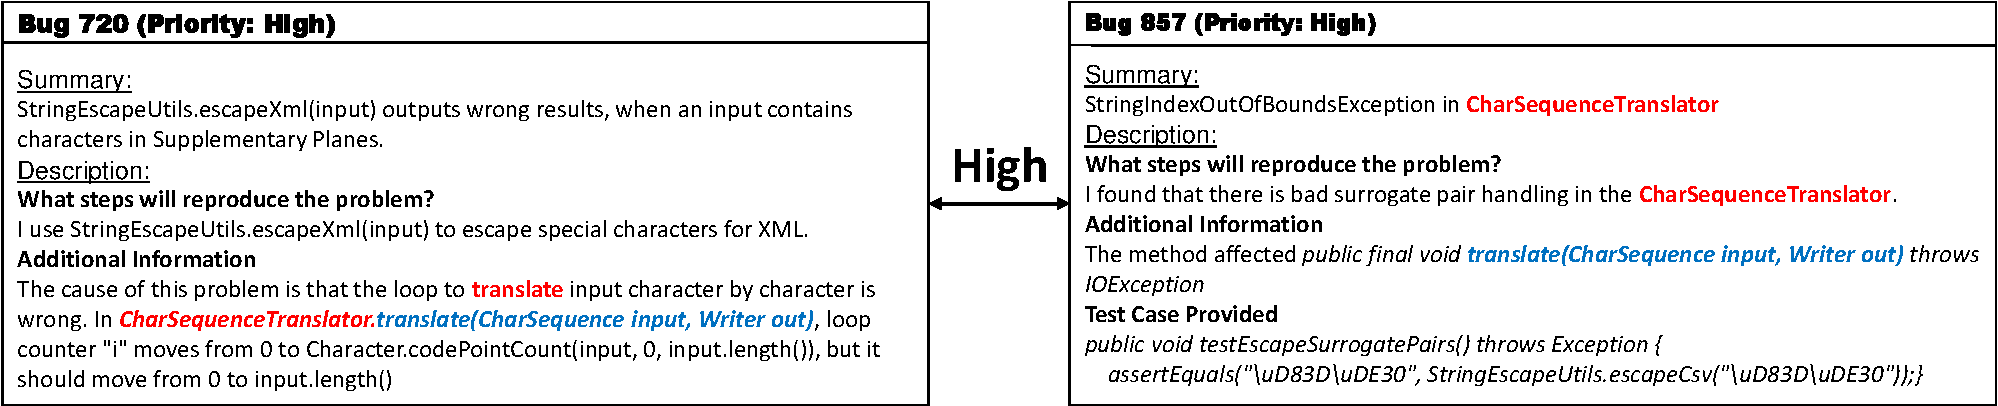
\includegraphics[width=0.55\textwidth]{bug_high_crop}
\caption{The proposed NetML framework}
\label{fig:bug_high}
\end{figure}

%\subsubsection{RQ5: Component Weights}\label{sec:rq3}
%%\begin{figure}[!htb]
%\centering
%
%\includegraphics[scale=0.5]{boxplot.eps}
%\caption{Contribution of $AML^{SPECTRA}$, $AML^{TEXT}$, and $AML^{BOTH}$}
%\label{fig:boxplot}
%\end{figure}

\begin{table}[!htb]
	\caption{Average Weights of Each Component }
	\centering
    \begin{tabular}{|c|c|c|c|}
    \hline
    \textbf{Project} & $\textbf{AML}^\textbf{Text}$ & $\textbf{AML}^{\textbf{SuspWord}}$ & $\textbf{AML}^\textbf{Spectra}$ \\ \hline\hline
AspectJ&-14.25&33.18&1.94\\\hline
Ant&9.14&12.5&1.54\\\hline
Lucene&12.43&25.77&-0.47\\\hline
Rhino&2.79&1.44&1.81\\\hline
    \end{tabular}
    \label{tab:contributions}
\end{table}

%In this research question, we investigate the contributions of $AML^{SPECTRA}$, $AML^{TEXT}$, and $AML^{BOTH}$ to the overall performance of the whole approach. We consider the default setting of $AML$, i.e., $n=20$. Figure~\ref{fig:boxplot} is the box plot showing the distribution of weights assigned to $AML^{SPECTRA}$, $AML^{TEXT}$, and $AML^{BOTH}$ which correspond to the values of $\alpha$, $\beta$, and $\gamma$ respectively. From the figure, we can note that for most bugs, all of the components are given non-zero weights. This shows that each component is important for a good number of bugs. Also, $AML^{BOTH}$ is often given higher weights than the other two components. The median weights given to $AML^{BOTH}$ and $AML^{SPECTRA}$ are the same, however the third quartile of the weights given to $AML^{BOTH}$ is much higher than the third quartile of the weights given to $AML^{SPECTRA}$. The mean of the weights given to $AML^{BOTH}$, $AML^{SPECTRA}$ and $AML^{TEXT}$ are 0.41, 0.32, and 0.27, respectively. 

%In this research question, we investigate the contribution of $\text{AML}^{\text{Text}}$, $\text{AML}^\text{SuspWord}$, and $\text{AML}^\text{Spectra}$ to the performance of AML in the context of the default setting (i.e., $n=10$). Table~\ref{tab:contributions} highlights the average weights of each AML component in the four projects.  From the Table~\ref{tab:contributions}, $\text{AML}^\text{SuspWord}$ has the highest weights than the other two components in AspectJ, Ant, and Lucene. For Rhino, $\text{AML}^\text{Text}$ has the highest weight (i.e., 2.79). Interestingly, according to Equation~\ref{eqn:composite}, component weights (i.e., $\alpha$, $\beta$, and $\gamma$) can be possible or negative numbers. From the table, AspectJ and Lucene are the two cases have negative component weights. Overall, we find that the component weights are well-tuned to maximize their contributions to the overall AML.

%[say something about the negative weights later ...]
We use default setting of AML ($n=10$) to evaluate contributions of component weights to the effectiveness of  AML. From Equation~\ref{eqn:composite}, we observe that component weights with large absolute values  have stronger influences on final suspiciousness scores of methods (i.e., $f(x_i, \theta)$), and near-zero weights have weaker influences on the suspiciousness scores. Based on our observation and the  result shown in Table~\ref{tab:contributions}, we find that average weights of AML$^\text{Text}$ and AML$^\text{SuspWord}$ in AspectJ, Ant, and Lucene are significantly larger than of AML$^\text{Spectra}$. This implies AML$^\text{Text}$ and AML$^\text{SuspWord}$ have stronger contribution to performance of AML than  AML$^\text{Spectra}$ in AspectJ, Ant, and Lucene. In Rhino, 
AML$^\text{Text}$ has the largest average weight, and AML$^\text{SuspWord}$ has the smallest weight. However, their differences are not significant compared to their magnitudes. Therefore, contributions of the three components to AML in Rhino are  relatively equivalent. On the other hand, AML$^\text{Text}$ and AML$^\text{Spectra}$ have negative average weights in AspectJ and Lucene, respectively. From Equation~\ref{eqn:composite}, we  observe that the purpose of negative weights is to decrease suspiciousness scores of methods when their magnitudes are much larger from the actual suspiciousness. Therefore, negative weights of SW$^\text{Text}$ and AML$^\text{Spectra}$ are for adjusting suspiciousness scores of methods to converge their actual values as much as possible.

%\subsection{RQ4: Adaptive vs. Non-Adaptive}\label{sec:rq4}
%%\begin{table}[t]
%	\centering
%	\caption{Adaptive vs. Non-Adaptive}
%    \begin{tabular}{|c|c|c|c|c|}
%    \hline
%      \textbf{Setting}& {\textbf{SR@1}} &\textbf{SR@5} &\textbf{SR@10} & \textbf{MAP} \\
%    \hline
%      \textbf{Adaptive} &{17.83\%}&{43.95\%}&{54.78\%}&\multirow{2}{*}{0.218}\\
%    ($AML$)   &(28)&(69)&(86)&\\\hline
%  \textbf{Non-Adaptive} &{???\%}&{???\%}&{???\%}&\multirow{2}{*}{???}\\
%	     ($AML_{*}$)  &(???)&(???)&(???)&\\\hline
%
%    
%    \end{tabular}
%    \label{tab:non_adaptive}
%\end{table}


\begin{table}[t]
	\centering
	\caption{Adaptive vs. Non-Adaptive}
	\scalebox{0.95}{
    \begin{tabular}{|c|c|c|c|c|c|}
    \hline
      \textbf{Project}& \textbf{Setting}&{\textbf{SR@1}} &\textbf{SR@5} &\textbf{SR@10} & \textbf{MAP} \\
    \hline
    \multirow{3}{*}{AspectJ} &$n=20$& 14.63\%&24.39\%&29.27\%&0.163   \\
    &$n=35$&19.51\%&26.83\%&31.71\%&0.199\\ 
    &$AML_{*}$&19.51\%&26.83\%&31.71\%&0.197\\\hline
     \multirow{3}{*}{Ant}  &$n=20$  &15.09\%&39.62\%&58.49\%&0.220 \\ 
&  $n=35$  &16.98\%&43.40\%&58.49\%&0.248\\
        &$AML_{*}$&13.21\%&41.51\%&58.49\%&0.228\\\hline
 \multirow{3}{*}{Lucene}& $n=20$ &29.73\%&64.86\%&75.68\%&0.284  \\ 
&$n=35$ &29.73\%&62.16\%&70.27\%&0.280\\
        &$AML_{*}$&29.73\%&62.16\%&70.27\%&0.280\\\hline
    \multirow{3}{*}{Rhino}&$n=20$   &11.54\%&53.85\%&57.69\%&0.204\\
    &$n=35$ &11.54\%&53.85\%&53.85\%&0.199\\
     & $AML_{*}$   &11.54\%&53.85\%&53.85\%&0.199\\\hline
    \textbf{ \multirow{3}{*}{Overall}}& $n=20$&17.83\%&43.95\%&54.78\%&0.218 \\
   
    &$n=35$ &19.75\%&45.22\%&53.50\%&0.234\\ 
      &$AML_{*}$ &18.47\%&44.59\%&53.50\%&0.227\\\hline
    \end{tabular}}
    \label{tab:non_adaptive}
\end{table}



\section{Discussion}
\label{sec:threats}

In this section, we discuss how NetML works in fault localization problem. We briefly show some examples and explain a case when NetML achieves good/poor performance. Moreover, there are several threats that may potentially impact the validity of our study. We also discuss these threats below.

\subsection{How does NetML work in Fault Localization?}
NetML contains two sets of latent parameters (i.e., bug reports and methods). The incorporation of the latent parameters provides NetML with a higher freedom to capture the relationship of different bug reports and methods more accurately. Moreover, NetML also employs the network Lasso regularization in its learning procedure, which imposes similar bug reports (and methods) to have similar latent parameters. Outputs of our NetML include the latent parameters of bug reports ($\mathbf{U}$) and methods ($\mathbf{V}$). Please refer to Section~\ref{sec:approach} for more details about NetML. 

Based on the latent parameters of bug reports (or methods), we apply cosine similarity~\cite{Salton:1975:VSM:361219.361220} to estimate how these bug reports are similar in latent space. Then we present some qualitative examples to illustrate the poor/good performance of NetML compared to other techniques. %More specifically, we show four case samples as follows:
%\begin{itemize}
%	\item A high cosine similar score of latent parameters between two bug reports. 
%	\item A low cosine similar score of latent parameters between two bug reports. 
%	\item A high cosine similar score of latent parameters between two methods. 
%	\item A low cosine similar score of latent parameters between two methods. 	
%\end{itemize}

\subsubsection{Case Examples of NetML: Good Results in Detecting Bugs}
\label{sec:case_good}
We introduce two examples defect to illustrate why NetML performs well in fault localization problem. We consider two bugs (i.e., Bug 720 and Bug 857) in project Lang. Bug 720 issues an ``outputs wrong results, when an input contains characters in \textit{Supplementary Planes}'' whereas Bug 857 contains ``\textit{StringIndexOutOfBoundsException}'' error. These two bugs ultimately reside in the \texttt{translate} method in the \texttt{CharSequenceTranslator.java} program. To find this method, based on the report, the developer could apply IR-based or spectrum-based bug localization techniques to generate a ranked list of methods. The list could then be inspected, in order, until the root cause of the bug is localized. Figure~\ref{fig:bug_high_crop} shows the description of two bugs (i.e., Bug 720 and Bug 857) in project Lang, which contains 5,528 methods. AML and SAVANT assign Bug 857 a high priority, i.e., localizing the \texttt{translate} method in the top 10 of the produced list. However, AML and SAVANT assign Bug 720 a low priority, i.e., localizing the \texttt{translate} method in the top 100 of the produced list. None of eight state-of-the-art spectrum fault localization techniques (i.e., OCHIAI, DSTAR, PROMESIR, DIT$^\text{A}$, DIT$^\text{B}$, LR$^\text{A}$, LR$^\text{B}$, and MULTRIC) localize the \texttt{translate} method within the top 10 of the produced list in both Bug 720 and Bug 857. The two best performance of spectrum fault localization approaches for this defect (i.e., OCHIAI and DSTAR) assigns the highest suspiciousness score to the faulty method; however, there are more than 100 methods sharing this score. Existing spectrum-fault localization approaches present limited utility for the developer in this case. 

On the other hand, NetML assigns Bug 720 and Bug 857 a high priority, which successfully localizes the faulty method (i.e., \texttt{translate}) within the top 10 of the produced list. Typically, we see that both NetML and AML assign Bug 857 a high priority. However, we assume that NetML takes advantages of the latent parameters of the two similar bug reports, and enforce them to have similar latent parameters. To explain our assumption, we apply a \textit{Vector Space Model} (VSM) to estimate the similarity between Bug 720 and Bug 857 at this space. We represent each bug report as vectors of weights; each weight corresponds a term. We evaluate the value of each weight by applying TF-IDF~\cite{Ramos1999} and estimate cosine similarity of Bug 857 with the remaining bug reports. We found that Bug 720 is ranked at position \textit{\#}39. We took the latent parameters of bug reports, which are the matrix $\mathbf{U}$ (please refer to Algorithm~\ref{alg:network_lasso}). We again estimate the cosine similarity of Bug 857 with the remaining bug reports in a latent space. In this case, Bug 720 is ranked at position \textit{\#}5. It shows that these two bugs are actually very close in the latent space. Indeed, these two bugs share the same \texttt{translate} method and  \texttt{CharSequenceTranslator} program, and these two bugs should be similar. AML only assumes that bug reports are independent, leading to failing to assign Bug 720 a high priority. On the other hand, NetML tries to enforce the similar bug reports to have similar latent parameters, leading to successfully to assign Bug 720 a high priority. 

Figure~\ref{fig:method_high_crop} presents the description of Bug 93 in project Time, which contains 4,181 methods. Bug 93 issues an error when ``weekyear has a null range duration type''. The bug resides in the \texttt{partial} and \texttt{compareTo} methods of the \texttt{Partial.java} and \texttt{UnsupportedDurationField.java} programs respectively. AML localizes the \texttt{partial} method in the top 5 of the produced list, however AML ranks the \texttt{compareTo} method at position \textit{\#}35. SAVANT also restricts the \texttt{partial} method in the top 10, and it ranks \texttt{compareTo} method at position \textit{\#}87. The spectrum fault localization techniques rank these two methods outside the top 100 of the produced list, which assigns this bug a low priority. NetML localizes the \texttt{partial} and \texttt{compareTo} methods at the rank \textit{\#}3 and \textit{\#}10 of the produced list respectively, which assigns Bug 93 a high priority. Similar to bug reports, we again calculate the similarity between two methods at the low space (vector space) and latent space. We collected the latent parameters of methods which are the matrix $\mathbf{V}$ (please refer to Algorithm~\ref{alg:network_lasso}). By applying VSM, we estimate cosine similarity of \texttt{partial} method with the remaining methods. We found that \texttt{compareTo} method is ranked at position \textit{\#}981. However, \texttt{compareTo} method is ranked at position \textit{\#}32 in the latent space. By looking at the content of these two methods, we see that they share the same parameter \texttt{DurationField} and \texttt{compareTo}, hence these methods should be close. AML assumes that methods are independent, leading to failing to localize the faulty \texttt{compareTo} method. NetML enforces the similar methods to have highly similar latent parameters, leading to successfully to localize \texttt{compareTo} method at rank \textit{\#}10. 

\subsubsection{Case Examples of NetML: Poor Results in Detecting Bugs}
\label{sec:case_bad}
We first introduce two examples defect to show why NetML achieves poor performance in fault localization problem. We consider Bug 617 and Bug 710 in project Lang. Bug 617 contains an error of ``process UTF-16 supplementary characters'' whereas Bug 710 has ``StringIndexOutOfBoundsException'' when we call a special string. These two bugs are related the \texttt{escapeXML} method in the \texttt{StringEscapeUtils.java} program. Figure~\ref{fig:bug_low} presents the details of these two bugs. NetML, AML, and SAVANT assign Bug 617 a high priority, however they fail to localize the faulty \texttt{escapeXML} method for Bug 710. Intuitively, \texttt{escapeXML} method and \texttt{StringEscapeUtils} program were clearly mentioned in Bug 617, hence should be easily captured by applying IR-based localization technique. OCHIAI and DSTAR estimate the highest suspiciousness score to the \texttt{escapeXML} method for both Bug 617 and Bug 710; however, we have around 50 methods sharing this score. The remaining baselines (i.e., PROMESIR, DIT$^\text{A}$, DIT$^\text{B}$, LR$^\text{A}$, LR$^\text{B}$, and MULTRIC) fail to localize these two bugs in a high priority. By reading the content of Bug 710, we see that this bug does not contain any information related to \texttt{escapeXML} method. Moreover, the suspiciousness score of the faulty method, which is calculated by using spectrum-fault localization, often shares with another methods. For these reasons, it is a challenge to assign a high priority for Bug 710. Similar to Section~\ref{sec:case_good}, we calculate the similarity score between these two bugs at low and latent spaces. We estimate the similarity of Bug 617 with the remaining bug reports. We found that Bug 710 is ranked at position \textit{\#}55 and \textit{\#}48 in the low level space and latent space, respectively. It shows that these two bugs are independently, and hence NetML fails to localize the faulty method for bug 710.

Figure~\ref{fig:method_low} shows the descriptions of Bug 18 in project Time. Bug 18 issues an null pointer exception when ``a DateTimeZone is build with duplicate-named''. The bug contains two faulty methods, i.e., \texttt{RuleSet} and \texttt{DateTimeOfYear}, in \texttt{ZoneInfoCompiler.java} program. NetML, AML, and SAVANT localizes the \texttt{RuleSet} method in the top 10 of produced list, however these techniques rank \texttt{DateTimeOfYear} method outside the top 50. OCHIAI and DSTAR rank these methods at the highest suspiciousness score, however we have 42 methods sharing this score. The other baselines fail to localize the two faulty methods within the top 50 of the produced list. We again estimate the similarity score between the two methods at a low level space and latent space. We calculate the similarity of method \texttt{RuleSet} against the remaining methods in Time. Method \texttt{DateTimeOfYear} is ranked at position \textit{\#} 2,678 and \textit{\#}2,468 in the low level space and latent space, respectively. It shows that these two methods independent with each other, hence NetML is unable to localize method \texttt{DateTimeOfYear}.

%\begin{figure*}[!t]
%	\centering
%	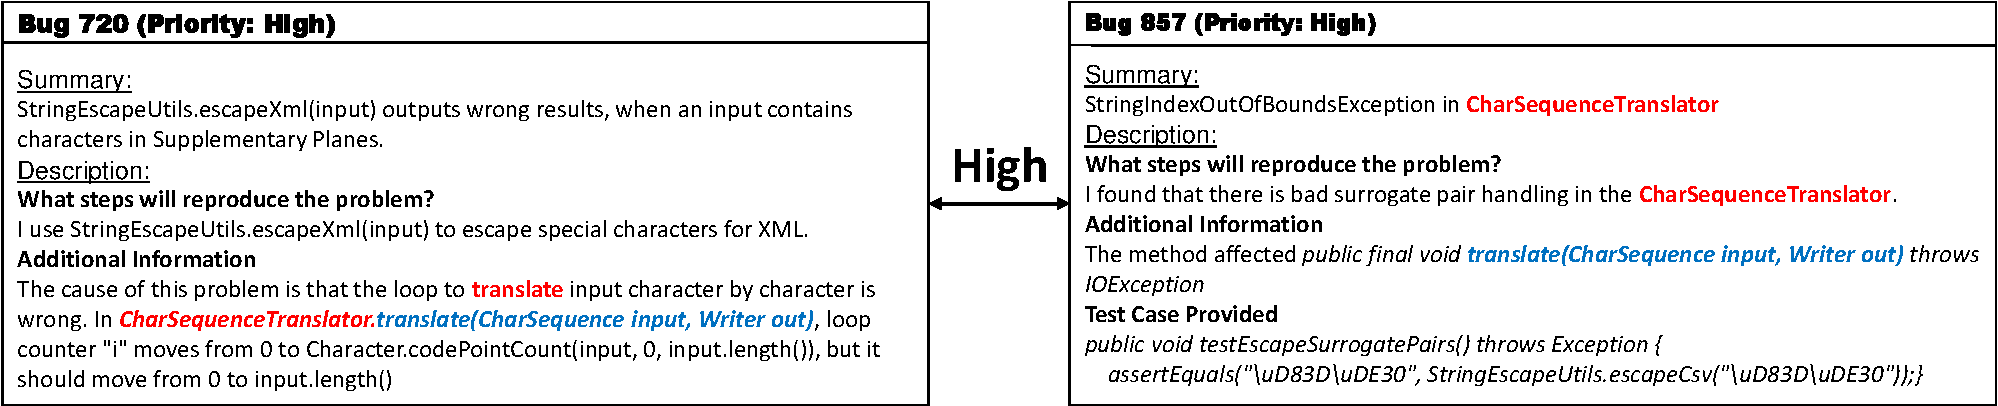
\includegraphics[width=\textwidth]{bug_high_crop}
%	\caption{The proposed NetML framework}
%	\label{fig:bug_high_crop}
%\end{figure*}

\begin{figure*}
	\centering
	\begin{subfigure}[b]{\textwidth}
		\centering
		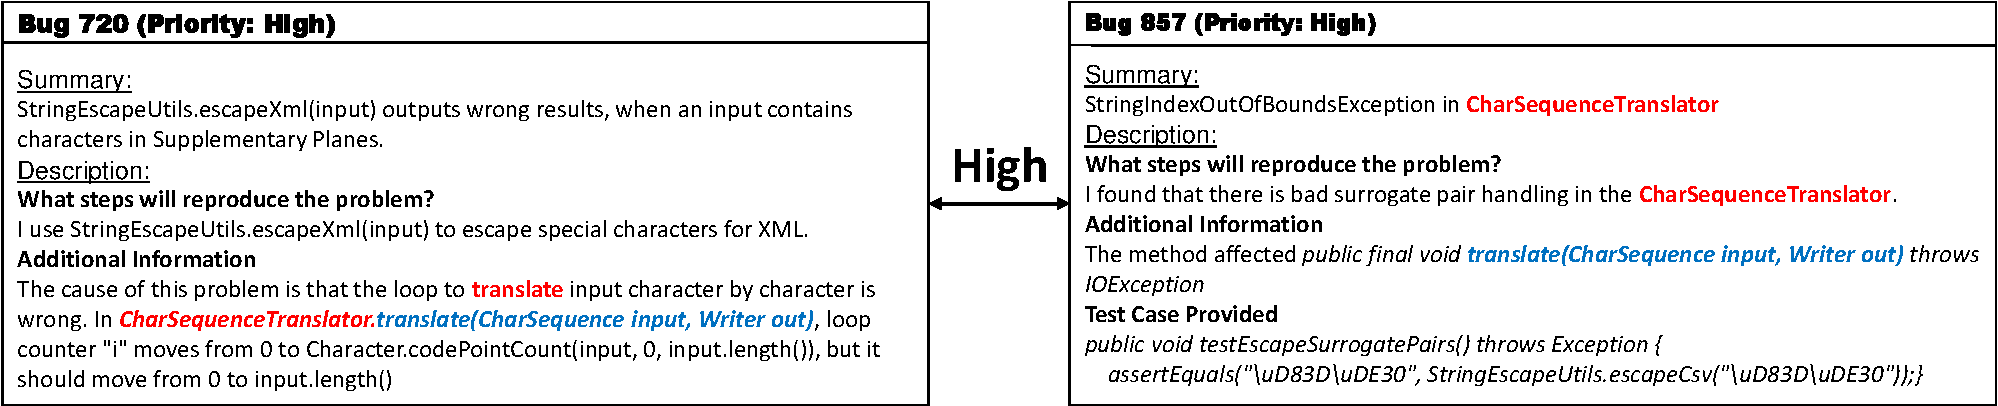
\includegraphics[width=\textwidth]{bug_high_crop}
		\caption[]%
		{{\small A case example which NetML achieves a good results. Two bug reports are highly similar at latent space.}}    
		\label{fig:bug_high_crop}
	\end{subfigure}
	\centering
	\begin{subfigure}[b]{\textwidth}  
		\centering 
		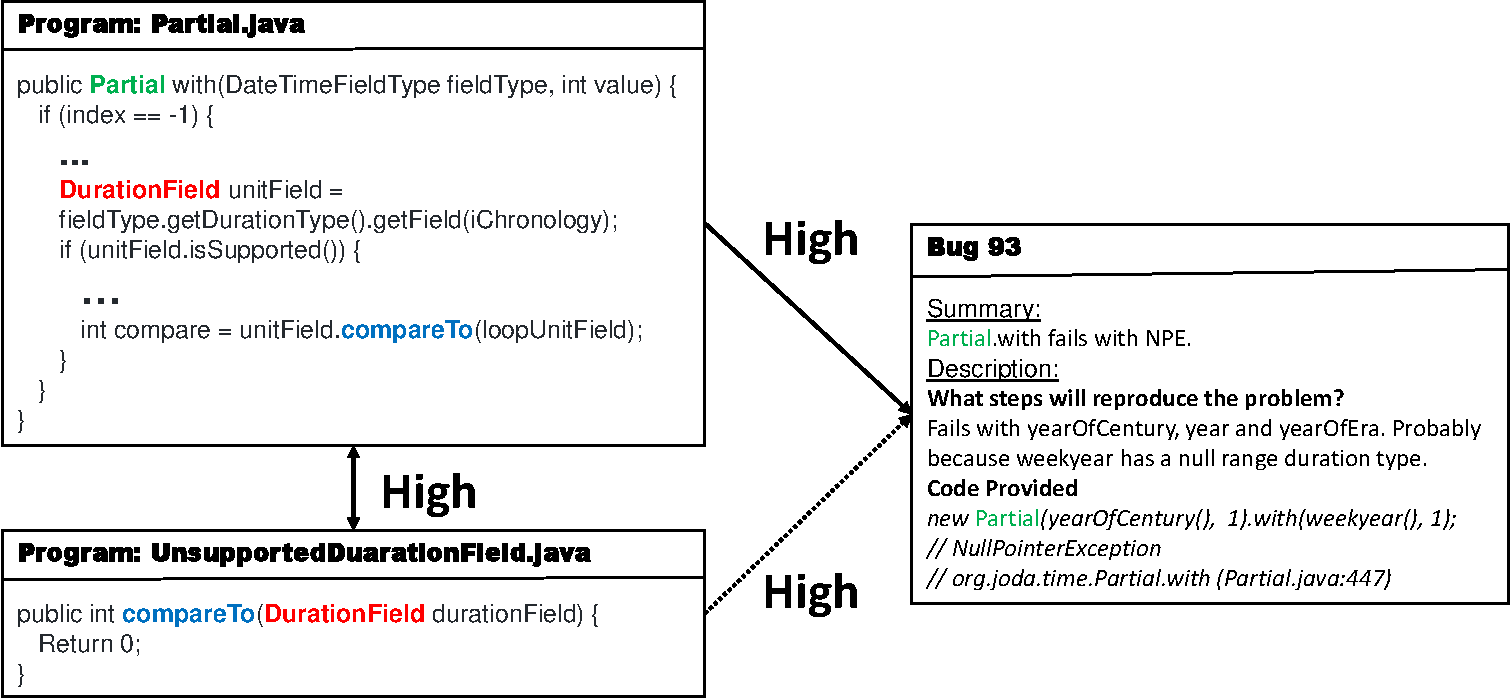
\includegraphics[width=\textwidth]{method_high_crop.pdf}
		\caption[]%
		{{\small A case example which NetML achieves a good results. Two methods are highly similar at latent space.}}    
		\label{fig:method_high_crop}
	\end{subfigure}
	\caption[]
	{\small A list of case examples to illustrate why NetML achieves good performance.}
\label{fig:case_good_example}

\end{figure*}
\begin{figure*}
	\centering
	\begin{subfigure}[b]{\textwidth}
		\centering
		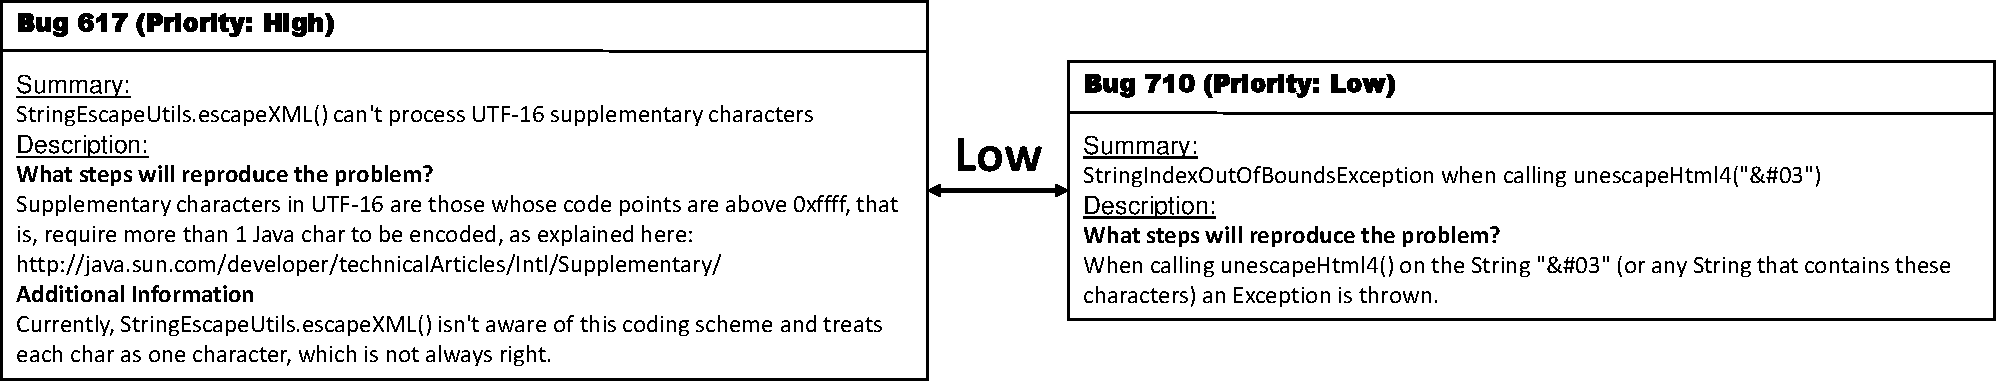
\includegraphics[width=\textwidth]{bug_low}
		\caption[]%
		{{\small A case example which NetML achieves a bad results. Two bug reports has a low similar at latent space.}}    
		\label{fig:bug_low}
	\end{subfigure}
	\centering
	\begin{subfigure}[b]{\textwidth}  
		\centering 
		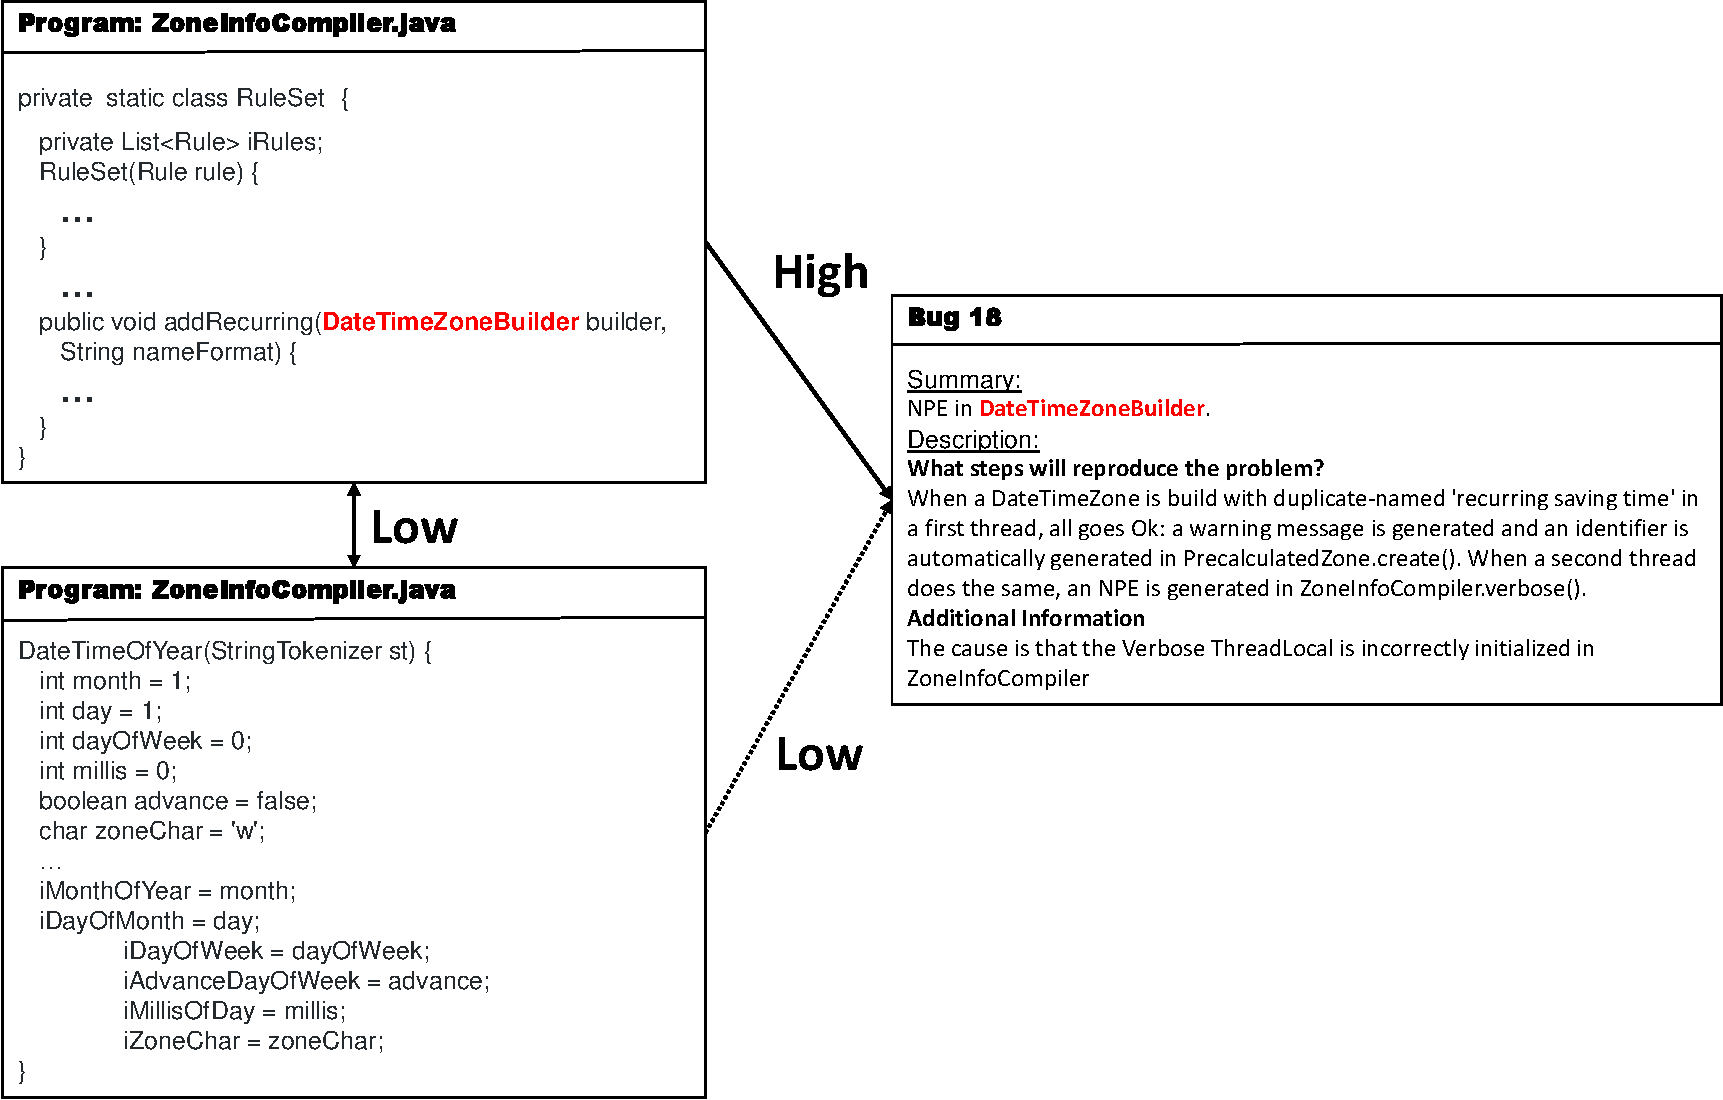
\includegraphics[width=\textwidth]{method_low_crop.pdf}
		\caption[]%
		{{\small A case example which NetML achieves a bad results. Two methods has a low similar at latent space.}}    
		\label{fig:method_low}
	\end{subfigure}
	\caption[]
	{\small A list of bad case examples to illustrate why NetML achievespoor performance.} 
	\label{fig:case_bad_example}
\end{figure*}





\subsection{Number of Failed Test Cases and Its Impact}

In our experiments with 157 bugs, most of the bugs were found to come with few failed test cases (average = 2.185). We have investigated if the number of failed test cases impacts the effectiveness of our approach. To this end, we computed the differences between the average number of failed test cases for bugs that are successfully localized at top-N positions (N = 1,5,10) and bugs that are not successfully localized. We found that the differences are small (-0.472 to 0.074 test cases). These indicate that the number of test cases does not impact the effectiveness of our approach significantly and typically 1 to 3 failed test cases are sufficient for our approach to be effective.

\subsection{Threats to Internal Validity} 

Threats to internal validity relate to implementation and dataset errors. We have checked our implementations and datasets. However, there could still be errors that we do not notice. Threats to external validity relate to the generalizability of our findings. In this work, we have analyzed 157 real bugs from 4 medium-large software systems. In the future, we plan to reduce the threats to external validity by investigating more real bugs from additional software systems, written in various programming languages. 

%\subsubsection{Threats to Construct Validity}
%
%Threats to construct validity relate to the suitability of our evaluation metrics and experimental settings. Both Top N and MAP have been used to evaluate many past bug localization studies~\cite{Rao:2011:RSL:1985441.1985451,Sisman:2012:IVH:2664446.2664454,Zhou:2012:BFM:2337223.2337226,SahaLKP13}. MAP is also well known in the information retrieval community~\cite{Manning2008}. We have performed cross validation to evaluate the effectiveness of approach on various training and test data. Cross validation is a standard setting used to evaluate many past studies~\cite{Anvik:2006:FTB:1134285.1134336,HooimeijerW07,DAmbrosLR10,ShivajiWAK13}. Unfortunately, cross validation ignores temporal ordering among bug reports. If bugs reported at different dates do not exhibit substantially different characteristics in terms of their program spectra and descriptions, then this threat is minimal.

%The creation of our datasets follow the heuristics described by Dallmeier and Zimmermann~\cite{DallmeierZ07}. These heuristics are not guaranteed to be perfect; for example, there could be some bug fixing commits that are not linked to their corresponding bug report. Still, all these systems are written in Java and open source. We also plan to investigate the effectiveness of our bug localization technique on closed-source or industrial software systems.
 
%Thus, we believe there is little threat to construct validity from evaluation metrics.

%Thus, we believe it is reasonable to ignore temporal ordering. In the future, we plan to evaluate our approach in different settings that captures date information of bug reports. \color{red}In addition to textual descriptions, bug reports contain date information (i.e., report dates) in their contents. These information can be used to construct a temporal order between bug reports. However, until now, it is unclear whether ordering of bug reports have impacts on root causes of bugs. For example, \textit{Null Pointer Exception} can happen anytime regardless the occurrences of  other bugs.}


\section{Related Work}\label{sec.related}
\section{Related Work}
\label{sec.related}

In this section, we highlight a number of research studies that are closely related to our work.
%Due to a large number of works in these areas, the survey here is by no means complete. We only highlight the closely related works.
%For a more complete coverage of studies on bug localization, please refer to the survey papers by Dit et al.~\cite{DitRGP13}.

\subsection{Multi-Modal Feature Location} 

Multi-modal feature location takes as input a feature description and a program spectra, and finds program elements that implement the corresponding feature. There are several multi-modal feature location techniques proposed in the literature~\cite{PoshyvanykGMAR07,LiuMPR07,DitRP13}.

Poshyvanyk et al. proposed an approach named PROMESIR that computes weighted sums of scores returned by an IR-based feature location solution (LSI~\cite{MarcusM03}) and a spectrum-based solution (Tarantula~\cite{JH05}), and rank program elements based on their corresponding weighted sums~\cite{PoshyvanykGMAR07}. Then, Liu et al. proposed an approach named SITIR which filters program elements returned by an IR-based feature location solution (LSI~\cite{MarcusM03}) if they are not executed in a failing execution trace~\cite{LiuMPR07}. Later, Dit et al. used HITS, a popular algorithm that ranks the importance of nodes in a graph, to filter program elements returned by SITIR~\cite{DitRP13}.
%They created a graph corresponding to a dynamic call graph that is generated from failed execution traces and use this graph as input to HITS.
Several variants are described in their paper and the best performing ones are $IR_{LSI}Dyn_{bin}WM_{HITS}(h,bin)^{bottom}$ and  $IR_{LSI}Dyn_{bin}WM_{HITS}(h,freq)^{bottom}$. We refer to these two as DIT$^A$ and DIT$^B$, respectively. They have showed that these variants outperform SITIR, though they have never been compared with PROMESIR.

In this work, we compare our proposed approach against PROMESIR, DIT$^A$ and DIT$^B$. We show that our approach outperforms all of them on all datasets.

\subsection{IR-Based Bug Localization} 

Various IR-based bug localization approaches that employ information retrieval techniques to calculate the similarity between a bug report and a program element (e.g., a method or a source code file) have been proposed~\cite{Rao:2011:RSL:1985441.1985451,Lukins:2010:BLU:1824820.1824850,LeWL13,Sisman:2012:IVH:2664446.2664454,Zhou:2012:BFM:2337223.2337226,SahaLKP13,WL14,WangLL14,YeBL14}. 

Lukins et al. used a topic modeling algorithm named Latent Dirichlet Allocation (LDA) for bug localization~\cite{Lukins:2010:BLU:1824820.1824850}. Then, Rao and Kak evaluated the use of many standard IR methods for bug localization including VSM and Smoothed Unigram Model (SUM)~\cite{Rao:2011:RSL:1985441.1985451}. In the IR community, VSM has a long history, proposed four decades ago by Salton et al.~\cite{SaltonWY75} and followed by many other IR methods including SUM and LDA, which address the limitations of VSM.

%They showed that simpler IR techniques, i.e., VSM and SUM, outperforms more complex ones including LDA. %{\color{red}Later, Le et al. apply multiple topic models inferred by Latent Dirichlet Allocation algorithm for IR-based bug localization~\cite{LeWL13}.} In the IR community, historically, VSM is proposed very early (four decades ago by Salton et al.~\cite{SaltonWY75}), followed by many other IR techniques, including SUM and LDA, which address the limitations of VSM.

More recently, a number of approaches which consider information aside from text in bug reports to better locate bugs were proposed. Sisman and Kak proposed a version history-aware bug localization method that considers past buggy files to predict the likelihood of a file to be buggy and uses this likelihood along with VSM to localize bugs~\cite{Sisman:2012:IVH:2664446.2664454}. Around the same time, Zhou et al.~\cite{Zhou:2012:BFM:2337223.2337226} proposed an approach named BugLocator that includes a specialized VSM (named rVSM) and considers the similarities among bug reports to localize bugs. Next, Saha et al.~\cite{SahaLKP13} developed an approach that considers the structure of source code files and bug reports and employs structured retrieval for bug localization, and it outperforms BugLocator. Wang and Lo proposed an approach that integrates the approaches by Sisman and Kak, Zhou et al. and Saha et al. for more effective bug localization~\cite{WL14}. Most recently, Ye et al. devised an approach named LR that combines multiple ranking features using learning-to-rank to localize bugs, and these features include surface lexical similarity, API-enriched lexical similarity, collaborative filtering, class name similarity, bug fix recency, and bug fix frequency~\cite{YeBL14}.
%{\color{red}  Ye~et~al.
%train word embeddings on API documents, tutorials, and reference documents to create additional semantic similarity features  for improving the effectiveness of IR-based bug localization~\cite{ye2016word}. Almhana~et~al. propose a multi-objective search  strategy leveraging  a fitness function that optimizes lexical-based similarity and
%history-based similarity to recommend relevant classes given a bug report~\cite{almhana2016recommending}.
%Wen~et~al. introduce \textit{Locus} that combine textual information from software changes hunks and source code files for locating bugs~\cite{wen2016locus}.
%}

 %The proposed approach named LR combines these ranking features by making use of an off-the-shelf learning-to-rank tool named SVM$^{rank}$.


%Wang and Lo further extended their approach by using a weighted composition of multiple VSM variants whose weights are learned using a genetic algorithm~\cite{WangLL14}.

All these approaches can be used as the AML$^\text{Text}$ component of our approach. In this work, we experiment with a basic IR technique namely VSM. Our goal is to show that even with the most basic IR-based bug localization component, we can outperform existing approaches including the state-of-the-art IR-based approach by Ye et al.~\cite{YeBL14}.

\subsection{Spectrum-Based Bug Localization} 

Various spectrum-based bug localization approaches have been proposed~\cite{JH05,Abreu:2009,LuciaLJB10,LuciaLJTB14, Libl+05,LYFHM05,Artzi2010,Artzi:2010:PFL:1806799.1806840,ZH02,Zeller2002a,CZ05,LuciaLX14}. These approaches analyze a program spectra which is a record of program elements that are executed in failed and successful executions, and generate a ranked list of program elements. Many of these approaches propose various formulas that can be used to compute the suspiciousness of a program element given the number of times it appears in failing and successful executions.

% Rephrase needed
Jones and Harrold proposed Tarantula that uses a suspiciousness score formula to rank program elements~\cite{JH05}. Later, Abreu et al. proposed another suspiciousness formula called Ochiai~\cite{Abreu:2009}, which outperforms Tarantula. Then, Lucia et al. investigated 40 different association measures and highlighted that some of them including Klosgen and Information Gain are promising for spectrum-based bug localization~\cite{LuciaLJB10,LuciaLJTB14}. Recently, Xie et al. conducted a theoretical analysis and found that several families of suspiciousness score formulas outperform other families~\cite{XieCKX13}. Next, Yoo proposed to use genetic programming to generate new suspiciousness score formulas that can perform better than many human designed formulas~\cite{Yoo12}. Subsequently, Xie et al. theoretically compared the performance of the formulas produced by genetic programming and identified the best performing ones~\cite{XieKCYH13}. Most recently, Xuan and Monperrus combined 25 different suspiciousness score formulas into a composite formula using their proposed algorithm named MULTRIC, which performs its task by making use of an off-the-shelf learning-to-rank algorithm named RankBoost~\cite{XuanM14}. MULTRIC has been shown to outperform the best performing formulas studied by Xie et al.~\cite{XieCKX13} and the best performing formula constructed by genetic programming~\cite{Yoo12,XieKCYH13}.
%{\color{red} More recently, Laghari~et~al. propose a variant of spectrum-based fault localization called as \textit{patterned spectrum analysis}, which leverages patterns of
%	method calls by means of frequent itemset mining~\cite{laghari2016fine}.
%Le~et~al. leverage  likely invariants inferred from  execution traces of passed and failed test cases and propose a learning-to-rank based framework called \textit{Savant} for localizing bugs~\cite{savant}. {\color{red} Pearson et~al. evaluate the effectiveness of 10 state-of-the-art bug localization techniques on more than 300 real faulty software program, as well as design a number of new mutation based bug localization techniques that are significantly more effective than existing existing approaches~\cite{PearsonCJFAEPK2017}.}
%}

%Later, Abreu et al. proposed another suspiciousness formula called Ochiai~\cite{Abreu:2009.jss}, which outperforms Tarantula. This formula is based on the intuition that program elements that are executed more often in failed executions than successful ones are more likely to be buggy.
%Next, Lucia et al. investigated the effectiveness of 40 different association measures proposed in the data mining community and highlighted that some of them including Klosgen and Information Gain are promising for spectrum-based bug localization~\cite{LuciaLJTB14}.

%~\cite{YooHC13}
%Artzi et al. addressed the issue of insufficient test cases for fault localization by a directed test generation technique~\cite{ADTP10a}. After the test cases were generated, they used Ochiai to evaluate their approach. Artzi et al. proposed another approach that extended Tarantula for debugging web applications~\cite{ArtziDTP10}.

%Aside from the above approaches that compute suspiciousness scores to program elements based on program spectra, there are many other approaches that also use program execution traces to localize bugs.  Zeller and Hildebrandt proposed Delta Debugging that generates failure-inducing inputs by performing a binary-search over the search space of possible inputs~\cite{ZH02}. Zeller applied Delta Debugging to analyze a failed and a successful execution trace to find the minimum state difference between them~\cite{Zeller2002a}. Cleve and Zeller proposed another tool named AskIgor which extends Delta Debugging with cause transitions, i.e., program locations where variables become new failure causes~\cite{CZ05}.

Many of the above mentioned approaches that compute suspiciousness scores of program elements can be used in the AML$^\text{Spectra}$ component of our proposed approach. In this work, we experiment with a popular spectrum-based fault localization technique namely Tarantula, published a decade ago, which is also used by PROMESIR~\cite{PoshyvanykGMAR07}. Our goal is to show that even with a basic spectrum-based bug localization component, we can outperform existing approaches including the state-of-the-art spectrum-based approach by Xuan and Monperrus~\cite{XuanM14}.



\subsection{Other Related Studies} 

There are many studies that compose multiple methods together to achieve better performance. For example, Kocaguneli et al. combined several single software effort estimation models to create more powerful multi-model ensembles~\cite{kocaguneli2012value}. Also, Rahman et al. used static bug-finding in order to improve the performance of statistical defect prediction (and vice versa)~\cite{rahman2014comparing}. Le~et~al. proposed SpecForge that combines different automaton based specification miners using  model fission and model fusion in order to create a more effective specification miner~\cite{le2015synergizing}.
Kellogg~et~al. presents \textit{N-Prog} that combines static bug detection and test case generation to avoid unnecessary human effort~\cite{Kellogg16}. In particular, \textit{N-Prog} produces no false alarms, by construction, since its output alarm is either a new test case or a bug in a program.

Recently, Perez~\cite{Perez:2017:TDM:3097368.3097446} proposed a new metric to quantify a test suite's diagnosability for spectrum-based fault localization. The goal is to optimize the effort to diagnose fault via spectrum-base techniques and guide the balance between unit tests and system test. On the other hand, Pearson~\cite{PearsonCJFAEPK2017} identified which fault localization techniques are the best of at finding real bugs and defined a new hybrid method that combining the best fault localization techniques based on 395 actual bugs. Wong~\cite{wong2016survey} provided a comprehensive overview of spectrum-fault localization techniques, and pointed out critical issues of software fault localization approach. 

%Additionally, there are  studies on the effectiveness of bug localization. Recently, Le et al. propose many frameworks to predict the effectiveness of IR-based and spectrum-based bug localization tools~\cite{LeL13,LeTL14,le2014should}.}


\section{Conclusion and Future Work} \label{sec.conclusion}
\section{Conclusion and Future Work}
\label{sec.conclusion}

In this paper, we put forward a novel multi-modal bug localization approach  named \underline{Net}work-clustered \underline{M}ulti-modal Bug \underline{L}ocalization (NetML). Deviating from the contemporary multi-modal localization approaches, NetML is able to achieve an effective bug localization through the interplay of two sets of latent parameters characterizing both bug reports and methods. It also features an adaptive learning procedure that stems from a strictly convex objective function formulation, thereby provides a sound theoretical guarantee on the uniqueness of the optimal solution.

We have extensively evaluated NetML on 157 real bugs from four different software projects (i.e., AspectJ, Ant, Lucene, and Rhino). Among the 157 bugs, NetML is able to successfully localize 46, 82, and 100 bugs when developers inspect the top 1, top 5, and top 10 methods, respectively. Compared to the best performing baseline (i.e., AML), NetML can successfully localize 48.39\%, 15.49\%, and 8.7\% more bugs when developers inspect the top 1, top 5, and top 10 methods, respectively. Furthermore, in terms of MAP, NetML outperforms the other baselines by 13.92\%. Based on the Wilcoxon signed-rank test using BH procedure, we show that the results of NetML are significantly better across the four projects, in terms of top 1, top 10, and MAP scores.

Although NetML offers a powerful bug localization approach, there remains room for improvement. For example, the current approach as well as the IR-based techniques capture both bug report and program element (method) using a simple bag-of-words (e.g., TF-IDF) representation, ignoring the inherent structure within the source codes of a program, such as function call and/or data dependencies. 
%only treated the methods as natural language by representing both the bug report and source code based on bag-of-words feature representations, and correlate the bug report and source code by measuring similarity in the same lexical feature space. 
In the future, we wish to consider a richer set of structural information within a program element, which carries additional semantics beyond the lexical terms. In particular, we would like to leverage both program structure information and lexical source code to localize potential bugs. We also plan to develop a more sophisticated technique, e.g., based on deep learning~\cite{Goodfellow2016}, to automatically learn the feature representation of bug reports and program elements.

%In this paper, we put forward a novel multi-modal bug localization approach named \underline{A}daptive \underline{M}ulti-modal bug \underline{L}ocalization (AML). Different from previous multi-modal approaches that are one-size-fits-all, our proposed approach can adapt itself to better localize each new bug report by tuning various weights learned from a set of training bug reports that are relevant to the new report. AML (in particular its \textit{AML}$^\textit{SuspWord}$ component) also leverages the concept of {\em suspicious words} (i.e., words that are associated to a bug) to better localize bugs. We have evaluated our proposed approach on 157 real bugs from 4 software systems. Our experiments highlight that, among the 157 bugs, AML can successfully localize 31, 71, and 92 bugs when developers inspect the top 1, top 5, and top 10 methods, respectively. Compared to the best performing baseline, AML can successfully localize 47.62\%, 31.48\%, and 27.78\% more bugs when developers inspect the top 1, top 5, and top 10 methods, respectively. Furthermore, in terms of MAP, AML outperforms the best baseline by 28.80\%.

%AML can successfully localize 31, 71, and 92 bugs when developers inspect the top 1, top 5, and top 10 methods, respectively. Compared to the best performing baseline (i.e., PROMESIR), AML can successfully localize 47.62\%, 31.48\%, and 27.78\% more bugs when developers inspect the top 1, top 5, and top 10 methods, respectively. Furthermore, in terms of MAP, AML outperforms the best baseline by 28.80\%. AML* is an extension framework of AML takes into account the similarity properties of bug reports and methods, and outperforms AML by 48.39\%, 15.49\%, and 8.7\% in the top 1, top 5, and top 10 methods. Moreover, AML* also outperforms AML by 13.9\% in terms of MAP scores.

%achieve an average MAP score of 0.237 and a success-count@1, success-count@5, and success-count@10 of 31, 72, and 92, respectively. These scores are better than the best performing baseline by 29.20\%, 47.62\%, 33.33\%, and 27.78\% for MAP, success-count@1, success-count@5, and success-rate@10, respectively.

%One of the components of AML (i.e., $AML^{SuspWord}$) leverages .  %Based on the observation of Parnin and Orso~\cite{ParninO11}, we also introduce and use the concept of word suspiciousness to identify buggy methods.
%To compute the suspiciousness of a method, our approach breaks the method into its constituent words, computes the suspiciousness scores of the constituent words, and combines these scores.
%Our proposed approach is thus analogous to a machine learning algorithm that breaks a data instance into its constituent features, computes the weights of these features, and combines the values of these features back to recommend a label for the data instance.

%In the future, we plan to improve the effectiveness of our proposed approach in terms of Top N and MAP scores. To reduce the threats to external validity, we also plan to investigate more bug reports from additional software systems. %which are implemented in different programming languages.

\vspace{0.2cm}\noindent{\bf Dataset and Codes.} Additional information on the 157 bugs used in the experiments can be found at \url{https://bitbucket.org/amlfse/amldata}. The codes of the NetML method can also be made available upon request.

%In the future, we plan to investigate more bug reports from additional software systems to increase generalizablity of our findings. {\color{red}We also plan to improve the effectiveness of our proposed approach further in order to achieve higher Top N score and Mean Average Precision. Information of the dataset is available at \url{google.com}.}


%\section{Acknowledgment}
%%\section{Acknowledgment}
%
%This research is supported by the National Research Foundation, Prime Minister’s Office, Singapore under its International Research Centres in Singapore Funding Initiative. 
\balance
\bibliographystyle{abbrv}
\bibliography{main,pbuglocator,faultlocal}
\end{document}
